\documentclass[twoside,a4paper,12pt]{report} %--- Druk dwustronny: twoside. Druk jednostronny: ondeside
\usepackage{polski}
\usepackage[utf8]{inputenc}
\usepackage{indentfirst}
\usepackage[protrusion=false]{microtype}
\DisableLigatures{encoding = *, family = * }
\usepackage{fancyhdr}
\usepackage{amssymb}
\usepackage{url,hyperref}
\hypersetup{
    colorlinks = true,
    linkcolor=.,
    citecolor=.,
    urlcolor = {blue}
}
\usepackage{multirow,multicol}
\usepackage[singlelinecheck=false,skip=2pt]{caption}
\usepackage{booktabs,float,tabularx,ltablex}
\usepackage[flushleft]{threeparttable}
\usepackage{enumitem}
\usepackage{pstricks,graphicx}
\usepackage{amsmath}
\usepackage[nottoc]{tocbibind}
\usepackage{natbib}
% \bibliographystyle{apalike}%--- Styl bibliograficzny APA 6th
\usepackage{lipsum}
\usepackage{chngcntr}
\counterwithout{table}{chapter}
\counterwithout{figure}{chapter}
\usepackage{titlesec}
\usepackage{tikz}
\usepackage{pgfplots}
\pgfplotsset{compat=1.14}
\floatstyle{plaintop}
\newfloat{wykres}{tbph}{loc}
\floatname{wykres}{Wykres}
\usepackage{cleveref}
\crefname{wykres}{wykres}{wykres}
\Crefname{wykres}{wykres}{Wykres}
\newcommand\listofcharts{\listof{wykres}{Spis wykresów}}
\usepackage{geometry}
\newgeometry{tmargin=2.5cm, bmargin=2.5cm, headheight=16pt, inner=2.5cm, outer=2.5cm} 
\usepackage{pdflscape}
\usepackage{rotating}
\usepackage{theorem}
\theoremstyle{break}
\theorembodyfont{\it}
\newtheorem{definition}{Definicja}[section]
\theorembodyfont{\rm}
\newtheorem{defi}{Definicja}[chapter]
\usepackage{tikz}
\usepackage{listings}
\usepackage[ruled,vlined,noend]{algorithm2e}
\usepackage{minted}
\usepackage{diagbox}
\SetAlgorithmName{Algorytm}{List of protocols}

%%%%%%%%%%%%%%%%%%%%%%% --- Ustawienia układu strony --- %%%%%%%%%%%%%%%%%%%%%%%

\pagestyle{fancy}
%---Druk jednostronny. Aby wyłączyć należy dodać % przed \. Aby włączyć należy usunąć % prze \.

%\fancyhead[C]{} 
%\fancyfoot[R]{\thepage}
%\fancyhead[L]{\scriptsize\leftmark}
%\fancyhead[R]{\scriptsize\rightmark}
%\cfoot[]{}
%\fancypagestyle{plain}{%
%\fancyhf{} % clear all header and footer fields
%\fancyfoot[R]{\textbf{\thepage}} % except the center
%\renewcommand{\headrulewidth}{0pt}
%\renewcommand{\footrulewidth}{0pt}}

\setcounter{secnumdepth}{4}
%---Druk dwustronny. Aby wyłączyć należy dodać % przed \. Aby włączyć należy usunąć % prze \.

\fancyhead[LE,RO]{\scriptsize\leftmark}
\fancyhead[RE,LO]{{\scriptsize \rightmark}}
\fancyfoot[CE,CO]{}
\fancyfoot[LE,RO]{\thepage}
\cfoot[]{}
\fancypagestyle{plain}{%
\fancyhf{} % clear all header and footer fields
\fancyfoot[LE,RO]{\textbf{\thepage}} % except the center
\renewcommand{\headrulewidth}{0pt}
\renewcommand{\footrulewidth}{0pt}}

%%%%%%%%%%%%%%%%%%%%%%% --- Koniec edycji układu strony. Proszę nie edytować --- %%%%%%%%%%%%%%%%%%%%%%%
\renewcommand{\chaptermark}[1]{%
\markboth{\MakeUppercase{%
\chaptername}\ \thechapter.%
\ #1}{}}
\renewcommand{\sectionmark}[1]{\markright{\thesection.\ #1}}

%%%%%%%%%%%%%%%%%%%%%% --- Wypełnia student --- %%%%%%%%%%%%%%%%%%%%%%%

\title{Algorytmy Aproksymacyjne na Grafach Planarnych}
\author{Mikołaj Twaróg}
\date{2021}


%%%%%%%%%%%%%%%%%%%%%%% --- Formatowanie strony tytułowej --- %%%%%%%%%%%%%%%%%%%%%%%
\begin{document}
\titleformat{\chapter}[display] {\normalfont\Huge\bfseries}{\chaptertitlename\ \thechapter}{0pt}{\Huge}
\titlespacing{\chapter}{1cm}{2cm}{1cm}

\thispagestyle{empty}
\begin{center}{\sc \large
Uniwersytet Jagielloński\par\vspace{0.2cm}\par}
{\LARGE
INSTYTUT INFORMATYKI ANALITYCZNEJ}\par\vspace{0.2cm}\par
{\large
Studia stacjonarne}\par\vspace{1cm}\par
{\Large
Praca licencjacka}%--- Wypełnia student --- "Praca licencjacka" w przypadku prac licencjackich 
\end{center}
\vspace{1.5cm}
\begin{flushleft}
{\large
Nr albumu: 1147537}%--- Wypełnia student
\end{flushleft}
\vspace{1.5cm}
\begin{center}
{\LARGE
Mikołaj Twaróg
}\par\vspace{0.9cm}\par
{\huge
Wielomianowe schematy aproksymacyjne dla problemów $\mathcal{NP}$-trudnych na grafach planarnych
}
\end{center}
\vspace{4cm}
\begin{flushright}

Opiekun pracy magisterskiej:\\
dr inż. Krzysztof Turowski%--- Wypełnia student
\end{flushright}
\vfill
\begin{center}
Kraków 2021%--- Wypełnia student
\end{center}


\leavevmode\thispagestyle{empty}\newpage
\centerline{\LARGE \bf Streszczenie}\par\vspace{1cm}\par

Ogólnie przyjęte jest, że problemów $\mathcal{NP}$-zupełnych nie da się rozwiązać w czasie wielomianowym. Jednak wiele z tych ma problemów ma praktyczne zastosowania, które wymagają szybszego czasu działania, dlatego od dziesięcioleci trwają prace nad stworzeniem algorytmów, które rozwiązują te problemy w czasie wielomianowym na specjalnych danych wejściowych lub dają przybliżone wyniki. Ta praca zostanie poświęcona jednemu z takich podejść, czyli technice Baker. 

Artykuł \emph{Approximation Algorithms for $\mathcal{NP}$-Complete Problems on Planar Graphs}, opublikowany w 1994 przez Brendę Baker, opisuje sposób rozwiązania wielu problemów $\mathcal{NP}$-trudnych w czasie liniowym na grafach planarnych. Polega on na rozdzieleniu grafy planarnego na grafy $k$-zewnętrznie planarne, policzeniu dokładnego wyniku na każdym z nich, a następnie połączeniu wyników. Takie podejście umożliwia dla wybranego $k$~znalezienie rozwiązania problemów maksymalizacyjnych wielkości $\frac{k}{k+1}$ optymalnego rozwiązania oraz dla problemów minimalizacyjnych wielkości $\frac{k+1}{k}$ optymalnego rozwiązania,  o ile istnieje odpowiedni algorytm dokładny dla grafów $k$-zewnętrznie planarnych.

W tym samym artykule Baker opisała liniowy algorytm liczący dokładny wynik dla grafów $k$-zewnętrznie planarnych dla dowolnego ustalonego $k$. Parę lat wcześniej, bo w~1988 roku Hans Bodlaender opublikował artykuł opisujący algorytm rozwiązujący ten sam problem i osiągający podobną złożoność obliczeniową.

Celem tej pracy jest implementacja techniki Baker z użyciem obu algorytmów (Baker i~Bodlaendera) oraz ocenę jej praktyczności, w szczególności rzeczywistego czasu działania.

Pierwszy rozdział pracy zostanie poświęcony definicjom potrzebnym do zrozumienia algorytmu oraz opisowi historii i aktualnych wyników kilku problemów, które da się rozwiązać techniką Baker. W drugim rozdziale zostanie opisany algorytm liniowy rozwiązujący te problemy na grafach $1$-zewnętrznie planarnych. W kolejnym rozdziale opiszemy uogólnienie tego algorytmu do grafów $k$-zewnętrznie planarnych działające w czasie $O(c^kn)$. Rozdział czwarty poświęcimy dokładnemu opisowi brakujących lub opisanych skrótowo kroków algorytmu Baker. Następny rozdział poświęcimy algorytmowi Bodlaendera oraz algorytmowi tworzenia dekompozycji drzewowej grafu $k$-zewnętrznie planarnego. W rozdziale szóstym opiszemy technikę Baker, a w ostatnim rozdziale porównamy algorytm Baker do algorytmu Bodlaendera pod kątem praktycznego wykorzystania, zarówno trudności implementacji, jak i efektywności działania.

\thispagestyle{empty} 
\newpage
\thispagestyle{empty} 

\thispagestyle{empty} 
\tableofcontents %-- automatyczny spis treści

%%%%%%%%%%%%%%%%%%%%% --- Zasadnicza treść rozprawy zaczyna się tutaj --- %%%%%%%%%%%%%%%%%%%%%

\chapter{Wprowadzenie}

\section{Pojęcia dotyczące grafów} \label{rozdzial_1}
Algorytmy, które opisujemy w tej pracy operują na tak zwanych grafach planarnych. Zacznijmy jednak od podstawowych pojęć z teorii grafów, z użyciem klasycznej terminologii grafowej m.in. za \cite{diestel}.

\begin{definition}[Graf]
\emph{Grafem} nazywamy parę $G=(V,E)$ zbiorów, takich, że $E \subseteq [V]^2$, więc elementy $E$ to dwuelementowe podzbiory $V$. Elementy $V$ będziemy nazywać wierzchołkami, a $E$ krawędziami.
\end{definition}

Liczbę wierzchołków w grafie będziemy oznaczać w pracy jako $n$, a liczbę krawędzi jako $m$.
Zakładamy ponadto, że graf otrzymany na wejście jest grafem prostym i bez pętli, czyli dla każdych dwóch krawędzi $\{a,b\},\{c,d\}\in E$ zachodzi $\{a,b\}\neq \{c,d\}$ oraz dla każdej krawędzi $\{a,b\}$ zachodzi $a\neq b$.

\begin{definition}[Incydencja wierzchołka]
W grafie $G=(V,E)$ wierzchołek $v \in V$ jest \emph{incydentny} z krawędzią $e \in E$, gdy $v \in e$.
\end{definition}

\begin{definition}[Stopień wierzchołka]
W grafie $G=(V,E)$ \emph{stopień wierzchołka} $v \in V$ to liczba krawędzi $e \in E$ incydentnych z nim. 
\end{definition}

\begin{definition}[Sąsiedztwo wierzchołków]
W grafie $G=(V,E)$ dwa wierzchołki $v,w \in V$ są \emph{sąsiednie}, gdy istnieje krawędź $\{v, w\} \in E$.
\end{definition}

\begin{definition}[Sąsiedztwo wierzchołka i zbioru]
Dla grafu $G$ i liczby $c \ge 0$ \emph{sąsiedztwem wierzchołka} $v$ będziemy nazywać zbiór wierzchołków znajdujących się w odległości co najwyżej $c$ od $v$ i będziemy zapisywać jako $N_c(v,G)$. \emph{Sąsiedztwem zbioru} $S \subseteq V$ będziemy nazywać zbiór wierzchołków w odległości co najwyżej $c$ od $S$, czyli $N_c(S,G)=\bigcup_{v \in S}N_c(v,G)$.
\end{definition}

Dla jednego z omówionych algorytmów potrzebne będą również pojęcia związane z~drzewem rozpinającym grafu oraz minorem grafu.

\begin{definition}[Drzewo rozpinające]
\emph{Drzewo rozpinające} grafu $G=(V,E)$ to $T=(V,F)$, gdzie $F$ jest maksymalnym podzbiorem $E$, takim że $T$ jest spójne oraz acykliczne. 
\end{definition}

\begin{definition}[Cykl bazowy]
Dla maksymalnego drzewa rozpinającego $T=(V,F)$ grafu $G=(V,E)$ \emph{cyklem bazowym} krawędzi $\{v,w\} \in E \setminus F$ nazywamy cykl składający się z krawędzi $\{v,w\}$ oraz ścieżki między $v$ i $w$ w $T$. Jako $vr(G,T)$ będziemy oznaczać maksimum ze wszystkich wierzchołków $G$ po liczbie cykli bazowych przechodzących przez wierzchołek.
\end{definition}

\begin{definition}[Minor]
Graf $G$ nazywamy minorem grafu $H$, jeśli graf $G$ może zostać stworzony z grafu $H$ poprzez serię usunięć wierzchołków, usunięć krawędzi oraz ściągnięć krawędzi, czyli operacji, która podmienia dwa sąsiednie wierzchołki $u,v$, wierzchołkiem, który jest sąsiedni do wszystkich wierzchołków, które sąsiadowały z $u$ lub $v$.
\end{definition}

W niniejszej pracy omawiane są algorytmy działające na konkretnej klasie grafów, czyli na grafach planarnych. Ograniczając się tylko do tej jednej klasy grafów wiele problemów udaje się rozwiązać szybciej, co zostało opisane w kolejnej sekcji tego rozdziału. Dodatkowo przydatną charakterystyką grafów planarnych jest to, że liczba krawędzi zależy w sposób liniowy od liczby wierzchołków, czyli dla grafu planarnego $G=(V,E)$ zachodzi $m \le 3n - 6$. Dzięki temu wszystkie algorytmy działające na ogólnej klasie grafów w czasie $O(n+m)$ na grafach planarnych działają w czasie $O(n)$. Pojęcia dla grafów planarnych są przywołane za \cite{math_dict} i \cite{emb}.

\begin{definition}[Graf planarny]
Graf planarny to graf, który możemy narysować na płaszczyźnie w taki sposób, aby żadne dwie krawędzie się nie przecinały.
\end{definition}
Co ciekawe, jeśli graf jest prosty, to możliwe jest narysowanie grafu planarnego na płaszczyźnie w taki sposób, żeby krawędzie były odcinkami.

\begin{definition}[Embedding geometryczny]
\emph{Embedding geometryczny} to przedstawienie grafu planarnego na płaszczyźnie, każdemu wierzchołkowi przyporządkowany jest inny punkt na płaszczyźnie, a każdej krawędzi krzywa Jordana, w taki sposób że krzywe są parami rozłączne.
\end{definition}

\begin{definition}[Ściana]
Embedding geometryczny grafu dzieli płaszczyznę na regiony. Każdy taki region będziemy nazywać \emph{ścianą}. Istnieje jeden nieograniczony region, który będziemy nazywać ścianą zewnętrzną.
\end{definition}

\begin{figure}[ht]
\begin{center}
    

\tikzset{every picture/.style={line width=0.75pt}} %set default line width to 0.75pt        

\begin{tikzpicture}[x=0.75pt,y=0.75pt,yscale=-1,xscale=1]
%uncomment if require: \path (0,300); %set diagram left start at 0, and has height of 300


% Text Node
\draw (173,146) node [anchor=north west][inner sep=0.75pt]   [align=left] {0};
% Text Node
\draw (247,46) node [anchor=north west][inner sep=0.75pt]   [align=left] {1};
% Text Node
\draw (370,146) node [anchor=north west][inner sep=0.75pt]   [align=left] {2};
% Text Node
\draw (226,239) node [anchor=north west][inner sep=0.75pt]   [align=left] {3};
% Text Node
\draw (321,239) node [anchor=north west][inner sep=0.75pt]   [align=left] {4};
% Text Node
\draw (231,167) node [anchor=north west][inner sep=0.75pt]   [align=left] {5};
% Text Node
\draw (282,113) node [anchor=north west][inner sep=0.75pt]   [align=left] {6};
% Text Node
\draw (292,167) node [anchor=north west][inner sep=0.75pt]   [align=left] {7};
% Text Node
\draw (214,129) node [anchor=north west][inner sep=0.75pt]   [align=left] {$\displaystyle a$};
% Text Node
\draw (256,113) node [anchor=north west][inner sep=0.75pt]   [align=left] {$\displaystyle b$};
% Text Node
\draw (312,130) node [anchor=north west][inner sep=0.75pt]   [align=left] {$\displaystyle c$};
% Text Node
\draw (270,148) node [anchor=north west][inner sep=0.75pt]   [align=left] {$\displaystyle d$};
% Text Node
\draw (249,192) node [anchor=north west][inner sep=0.75pt]   [align=left] {$\displaystyle e$};
% Text Node
\draw (308,211) node [anchor=north west][inner sep=0.75pt]   [align=left] {$\displaystyle f$};
% Text Node
\draw (336,69) node [anchor=north west][inner sep=0.75pt]   [align=left] {$\displaystyle z$};
% Connection
\draw    (333.09,235) -- (368.91,167) ;
% Connection
\draw    (367,147.59) -- (261,61.41) ;
% Connection
\draw    (244,65.99) -- (187,143.01) ;
% Connection
\draw    (185.62,167) -- (224.38,235) ;
% Connection
\draw    (240,242.01) -- (367,159.99) ;
% Connection
\draw    (240,247.5) -- (318,247.5) ;
% Connection
\draw    (250.85,67) -- (238.15,163) ;
% Connection
\draw    (228,172.42) -- (187,157.58) ;
% Connection
\draw    (295.19,163) -- (289.81,134) ;
% Connection
\draw    (289,175.5) -- (245,175.5) ;
% Connection
\draw    (306,173.21) -- (367,156.79) ;
% Connection
\draw    (280.97,109) -- (259.03,67) ;
% Connection
\draw    (279,130.5) -- (245,166.5) ;

\end{tikzpicture}

\end{center}
\caption{Przykładowy graf planarny ze ścianami oznaczonymi literami od $a$ do $f$ i $z$.}
\label{sciany}
\end{figure}

Każdą ścianę możemy również reprezentować jako listę wierzchołków w następujący sposób: zaczynając od dowolnego wierzchołka przechodzimy kolejne wierzchołki i krawędzie ograniczające ścianę w taki sposób, że ściana leży cały czas po prawej stronie krawędzi. Na przykład na rysunku \ref{sciany} możemy przedstawić ścianę $c$ jako listę $[1,2,7,6]$, a ścianę zewnętrzną $z$ jako $[0,3,4,2,1]$.

\begin{definition}[Sąsiedztwo ścian]
W embeddingu grafu $G=(V,E)$ dwie ściany $f_1, f_2$ są \emph{sąsiednie}, gdy istnieje krawędź $e \in E$, taka że $e \subseteq f_1$ i $e \subseteq f_2$. 
\end{definition}

\begin{definition}[Embedding kombinatoryczny]
Embedding geometryczny grafu indukuje cykliczną kolejność krawędzi sąsiadujących z~ustalonym wierzchołkiem. Graf z ustaloną kolejnością krawędzi dla każdego wierzchołka to \emph{embedding kombinatoryczny}.
\end{definition}

Dwa embeddingi geometryczne tego samego grafu $G$ nazywamy równoważnymi jeśli indukują ten sam embedding kombinatoryczny oraz te same wierzchołki należą do ich ścian zewnętrznych. Embedding kombinatoryczny z wybraną ścianą zewnętrzną jest równoważny tak zdefiniowanej klasie równoważności embeddingów geometrycznych. W~niniejszej pracy embedding kombinatoryczny z wyznaczoną ścianą zewnętrzną będziemy nazywać embeddingiem.

Jako pomocnicza klasa grafów zostały wykorzystane grafy $k$-zewnętrznie planarne. Specyficzny charakter tych grafów powoduje, że nawet problemy $\mathcal{NP}$-trudne stają się rozwiązywalne dla nich w czasie wielomianowym, co opisujemy w dalszej części pracy. Definicje dla tych grafów pochodzą z \cite{ioannis}, \cite{baker} oraz \cite{dominating}.

\begin{definition}[Graf $k$-zewnętrznie planarny]
Embedding grafu $G$ jest \emph{$1$-zewnętrznie planarny}, jeśli jest planarny i wszystkie jego wierzchołki leżą na ścianie zewnętrznej. Dla $k \ge 2$, embedding grafu $G$ jest \emph{$k$-zewnętrznie planarny}, jeśli po usunięciu wszystkich wierzchołków leżących na ścianie zewnętrznej zostaje nam embedding grafu $(k-1)$-zewnętrznie planarnego. Graf jest \emph{$k$-zewnętrznie planarny}, jeśli ma $k$-zewnętrznie planarny embedding.
\end{definition}

\begin{definition}[Poziomy wierzchołków dla embeddingu grafu planarnego]
Niech $L_1$ to zbiór wszystkich wierzchołków leżących na ścianie zewnętrznej embeddingu. Dla $i \ge 2$ definiujemy $L_i$ jako zbiór wierzchołków znajdujących się na ścianie zewnętrznej po usunięciu wszystkich wierzchołków ze zbiorów $L_j$, $1 \le j < i$. Wierzchołek $v$ jest poziomu $i$, gdy $v \in L_i$.
\end{definition}

\begin{definition}[Komponent]
Podgraf indukowany składający się z wierzchołków leżących na zewnętrznej ścianie grafu będziemy nazywać \emph{komponentem o poziomie $1$}. Podgraf indukowany składający się z~wierzchołków o poziomie $i+1 \ge 2$ znajdujących się wewnątrz ściany o poziomie $i$ będziemy nazywać \emph{komponentem o poziomie $(i+1)$}.
\end{definition}

\begin{definition}[Obszar między ścianą a komponentem]
Obszarem między ścianą a komponentem nazywamy region ściany z wycięciem regionu, który zajmuje komponent.
\end{definition}

Przykładowo, na rysunku \ref{sciany} wewnątrz ściany $[0,1,2,3]$ znajduje się komponent $\{5,6,7\}$, a obszar między między nimi składa się ze ścian $a$, $b$, $c$ i $e$.

Jeden z algorytmów prezentowanych w tej pracy nie operuje wprost na grafie danym na wejściu, lecz na stworzonej z niego dekompozycji drzewowej.

\begin{definition}[Dekompozycja drzewowa]
Dekompozycja drzewowa grafu $G=(V,E)$ to para uporządkowana $(\{X_i\colon i \in I\}, T)$, gdzie $\{X_i\colon i \in I\}$ to rodzina podzbiorów zbioru $V$, a $T=(I,F)$ to drzewo, takie, że:
\begin{itemize}
    \item $\bigcup X_i = V$,
    \item dla każdej krawędzi $\{v,w\} \in E$ istnieje takie $i \in I$, że $v \in X_i$ i $w \in X_i$,
    \item dla każdych $i,j,k \in I$, jeśli $j$ leży na ścieżce między $i$ i $k$, to $X_i \cap X_k \subseteq X_j$.
\end{itemize}
\end{definition}

\begin{definition}[Szerokość drzewowa]
\emph{Szerokość drzewowa dekompozycji drzewowej} $(\{X_i\colon i \in I\}, T=(I,F))$ to $\max_{i \in I} |X_i|-1$. \emph{Szerokość drzewowa grafu $G$} to najmniejsza szerokość drzewowa spośród wszystkich dekompozycji drzewowych grafu $G$.
\end{definition}

\section[Problemy NP-trudne]{Problemy $\mathcal{NP}$-trudne} \label{sekcja_1.2}
W tej pracy zajmiemy się trzema problemami $\mathcal{NP}$-trudnymi: znajdowaniem największego zbioru niezależnego, najmniejszego pokrycia wierzchołkowego oraz najmniejszego zbioru dominującego. W tym podrozdziale przedstawimy ich formalne definicje wraz z~dotychczas otrzymanymi wynikami na wszystkich grafach oraz przy ograniczeniu do grafów planarnych. 

Pierwszym problemem, którym się zajmiemy, jest szukanie największego zbioru niezależnego, które zostało opisane przez Baker w najdokładniejszy sposób.

\begin{definition}[Zbiór niezależny \cite{graph}]
Dla grafu $G=(V,E)$ \emph{zbiorem niezależnym} nazywamy podzbiór wierzchołków $U \subseteq V$, taki że dla każdych dwóch wierzchołków $x,y \in U$ zachodzi $\{x,y\} \notin E$.
\end{definition}

\begin{definition}[Zbiór niezależny \textendash\ problem decyzyjny]
Dostając na wejściu nieskierowany graf $G$ oraz liczbę naturalną $k$ zwracamy \texttt{tak}, jeśli dla grafu $G$ istnieje zbiór niezależny o mocy $k$, i \texttt{nie} w przeciwnym przypadku.
\end{definition}

\begin{definition}[Największy zbiór niezależny]
Dla grafu $G$ zwracamy największe takie $k$, że problem decyzyjny zbioru niezależnego dla $G$ i $k$ zwróci \texttt{tak}.
\end{definition}

Najłatwiejszym sposobem znalezienia zbioru niezależnego jest sprawdzenie każdego podzbioru wierzchołków, co można osiągnąć w czasie $O(2^nn)$. Dotychczas najlepsza złożoność została osiągnięta przez Xiao i Nagamochi w 2013 roku i wynosiła ona $(O(1.1996^nn^{O(1)}))$ \cite{xiao}. Dodatkowo w tym samym artykule zostały przedstawione dla grafu o największym stopniu wierzchołka $6$ i $7$ mające odpowiednio złożoność $O(1.1893^nn^{O(1)})$ i $O(1.1970^nn^{O(1)})$. Z drugiej strony, zakładając $\mathcal{P} \neq \mathcal{NP}$ nie da się stworzyć algorytmu aproksymacyjnego ze stałym współczynnikiem aproksymacji dla problemu największego zbioru niezależnego \cite{fpt}. Istnieje jednak prosty algorytm zachłanny dający rozwiązanie $\left(\frac{1}{\Delta + 1}\right)$-przybliżone, gdzie $\Delta$ to największy stopień wierzchołka w grafie.

Ograniczenie się do grafów planarnych nie pomaga w dokładnym wyznaczeniu największego zbioru niezależnego. Co więcej zostało udowodnione, że jest on $\mathcal{NP}$-trudny nawet gdy rozważamy tylko grafy planarne o największym stopniu wierzchołka mniejszym bądź równym $3$ \cite{max_ind}. Z drugiej strony, dla grafów planarnych istnieją dużo bardziej efektywne algorytmy aproksymacyjne. W 1982 Chiba, Nishizeki i Saito opracowali taki algorytm działający w złożoności $O(n\log n)$. Niestety dawał on w najgorszym przypadku wynik równy jedynie połowie wyniku optymalnego \cite{chiba}. Inne podejście zostało opracowane przez Liptona i Tarjana w 1980 roku. Uzyskali oni wynik $1 - O(\frac{1}{\sqrt{f(n)}})$-przybliżony w złożoności $O(n \max(\log n, 2^{f(n)}))$ \cite{lipton}. Podstawiając $f(n) = \log \log n$ dostajemy algorytm działający w czasie $O(n \log n)$ i $1 - O(\frac{1}{\sqrt{\log \log n}})$-przybliżony. Niestety w takim przypadku dostajemy rozwiązanie będące co najmniej połową optymalnego rozwiązania dopiero przy grafie o $2^{2^{400}}$ wierzchołkach \cite{chiba2}, co czyni ten algorytm całkowicie niepraktycznym.

Kolejnym znanym problemem $\mathcal{NP}$-trudnym, który chcemy rozważyć, jest problem znalezienia najmniejszego pokrycia wierzchołkowego.

\begin{definition}[Pokrycie wierzchołkowe \cite{graph}]
Dla grafu $G=(V,E)$ pokryciem wierzchołkowym nazywamy podzbiór wierzchołków $U \subseteq V$, taki że dla każdej krawędzi $\{x,y\} \in E$ zachodzi $x \in U$ lub $y \in U$.
\end{definition}

\begin{definition}[Pokrycie wierzchołkowe \textendash\ problem decyzyjny]
Dostając na wejściu nieskierowany graf $G$ oraz liczbę naturalną $k$ zwracamy \texttt{tak}, jeśli dla grafu $G$ istnieje pokrycie wierzchołkowe o mocy $k$ i \texttt{nie} w przeciwnym przypadku.
\end{definition}

\begin{definition}[Najmniejsze pokrycie wierzchołkowe]
Dla grafu $G$ zwracamy najmniejsze takie $k$, że problem decyzyjny pokrycia wierzchołkowego dla $G$ i $k$ zwróci \texttt{tak}.
\end{definition}

Tak samo jak największy zbiór niezależny, najmniejsze pokrycie wierzchołkowe możemy znaleźć rozważając wszystkie podzbiory wierzchołków w czasie $O(2^nn)$. W 2001 roku Robson pokazał algorytm dynamiczny znajdujący dokładny wynik w czasie $O(2^{\frac{n}{4}})$ \cite{robson}. Istnieje też prosty algorytm zachłanny umożliwiający w czasie liniowym policzenie pokrycia wierzchołkowego co najwyżej dwa razy większego niż rozwiązanie optymalne. 

W 2005 Demaine, Fomin, Hajiaghayi i Thilikos przedstawili schemat algorytmu, który umożliwia rozwiązanie wielu problemów $\mathcal{NP}$-trudnych (m.in. największego zbioru dominującego, najmniejszego maksymalnego skojarzenia, najmniejszego zbioru wierzchołków rozrywających cykle), w szczególności potrafi znaleźć pokrycie wierzchołkowe wielkości $k$ w czasie $O(2^{O(\sqrt{k})}n^{O(1)})$ \cite{erik}. Dla grafów planarnych możliwe jest również znalezienie lepszych algorytmów aproksymacyjnych. W 1982 roku Bar-Yahuda i Even pokazali liniowy algorytm dający rozwiązanie wielkości co najwyżej $\frac{5}{3}$ optymalnego rozwiązania \cite{bar}. W tym samym artykule pokazali oni również wielomianowy schemat aproksymacyjny bazujący na algorytmie Liptona i Tarjana \cite{lipton}. Dla dowolnego stałego $\varepsilon > 0$ potrafi on znaleźć rozwiązanie wielkości co najwyżej $1 + \varepsilon$ optymalnego rozwiązania w czasie $O(n \log n)$ (ale niewielomianowo zależne od $\frac{1}{\varepsilon}$).

Ostatnim problemem rozważanym w niniejszej pracy jest problem najmniejszego zbioru dominującego.

\begin{definition}[Zbiór dominujący \cite{graph}]
Dla grafu $G=(V,E)$ \emph{zbiorem dominującym} nazywamy podzbiór wierzchołków $U \subseteq V$, taki że dla każdego wierzchołka $x \in V$, $x \in U$ lub istnieje takie $y \in U$, że $\{x,y\} \in E$.
\end{definition}

\begin{definition}[Zbiór dominujący \textendash\ problem decyzyjny]
Dla danego na wejściu grafu $G$ oraz liczby naturalnej $k$ zwracamy \texttt{tak}, jeśli dla grafu $G$ istnieje zbiór dominujący o mocy $k$ i \texttt{nie} w przeciwnym przypadku.
\end{definition}

\begin{definition}[Najmniejszy zbiór dominujący]
Dla grafu $G=(V,E)$ zwracamy najmniejsze takie $k$, że problem decyzyjny zbioru dominującego dla $G$ i $k$ zwróci \texttt{tak}.
\end{definition}

Analogicznie do poprzednich problemów najmniejszy zbiór dominujący możemy znaleźć poprzez sprawdzenie wszystkich podzbiorów wierzchołków w czasie $O(2^nn)$. Najlepszy dotychczas algorytm dokładnego wyznaczania działający w czasie $O(1.4969^n)$ został opisany przez Rooija i Bodlaendera w 2011 \cite{rooij}. Prosty algorytm zachłanny okazuje się być $(\ln{\Delta} + 2)$-przybliżony, gdzie $\Delta$ to największy stopień wierzchołka w grafie.
Zacytowany wcześniej schemat Demaine'a i in. \cite{erik} również może zostać wykorzystany do znalezienia zbioru dominującego wielkości $k$ w czasie $O(2^{O(\sqrt{k})}n^{O(1)})$.

Na grafach planarnych problem najmniejszego zbioru dominującego wciąż jest $\mathcal{NP}$-zupełny. Istnieją jednak algorytmy potrafiące znaleźć zbiór dominujący o rozmiarze co najwyżej $k$ dla dowolnego wybranego $k$ (jeśli taki zbiór istnieje). W 2002 roku Alber, Bodlaender, Fernau, Kloks i Niedermeier przedstawili taki algorytm działający w czasie $O(4^{6\sqrt{34k}}n)$ \cite{Alber2002}. W 2005 roku Alber, Fan, Fellows, Fernau, Niedermeier, Rosamond i Stege zaprezentowali dwa algorytmy działające odpowiednio w czasie $O(8^kn)$ i $O(8^kk+n^3)$ \cite{ALBER2005385}. 

Wobec $\mathcal{NP}$-trudności podanych wyżej problemów istotne jest opracowanie możliwie szybkich i dokładnych algorytmów przybliżonych. Jednym z podejść jest szukanie algorytmów umożliwiających sterowanie dokładnością działania, czyli tzw. schematów aproksymacyjnych.

\begin{definition} \label{def_schemat}
Schemat aproksymacyjny to algorytm, który dla danego na wejściu problemu optymalizacyjnego oraz wartości $\varepsilon > 0$ potrafi w czasie wielomianowym stworzyć rozwiązanie co najwyżej $1+ \varepsilon$ razy większe od rozwiązania optymalnego dla problemów minimalizacyjnych i co najwyżej $1-\varepsilon$ razy mniejsze od rozwiązania optymalnego dla problemów maksymalizacyjnych.
\end{definition}

Schemat aproksymacyjny działający w czasie wielomianowym od $n$ i potrafiący rozwiązać wszystkie wymienione powyżej problemy, jak również wiele innych, został przedstawiony przez Baker w 1982 roku. Bazuje on na podziale grafu planarnego na grafy $k$-zewnętrznie planarne, policzeniu dokładnego wyniku na każdym z nich oraz połączeniu wyników. W tej pracy opiszemy i porównamy dwa sposoby obliczenia dokładnego wyniku dla grafów $k$-zewnętrznie planarnych: algorytm przedstawiony przez Baker razem ze schematem aproksymacyjnym oraz algorytm Bodlaendera korzystający z dekompozycji drzewowej grafu.

W dalszej części pracy będziemy nazywać schemat aproksymacyjny Baker techniką Baker, a algorytm wyliczania dokładnego rozwiązywania na grafach $k$-zewnętrznie planarnych algorytmem Baker.  



\chapter[Liniowy algorytm na grafach 1-zewnętrznie planarnych]{Liniowy algorytm na grafach \\ $1$-zewnętrznie planarnych} \label{sec.zewn}
Zacznijmy od przedstawienia algorytmu podanego w pracy Baker, który umożliwia rozwiązanie takich problemów jak zbiór niezależny, pokrycie wierzchołkowe czy zbiór dominujący na grafach $1$-zewnętrznie planarnych. Podejście to uogólnimy później dla grafów $k$-zewnętrznie planarnych.

Na początek, mając spójny graf $1$-zewnętrznie planarny zduplikujmy każdą krawędź będącą mostem, co spowoduje powstanie w tym miejscu ściany. Nazwijmy tak powstały graf $G$. Schemat nasz będzie polegał na zbudowaniu ukorzenionego drzewa $T$ (wierzchołki $T$ będziemy nazywać węzłami dla odróżnienia ich od wierzchołków $G$) na podstawie grafu $G$ oraz na dynamicznym wyliczaniu wartości w węzłach $T$.

Załóżmy najpierw, że nasz graf nie ma punktów artykulacji.
Konstrukcja $T$ będzie wyglądała następująco: stwórzmy wierzchołek dla każdej krawędzi zewnętrznej oraz wewnętrznej ściany grafu $G$. Węzeł reprezentujący ścianę $f$ połączmy ze wszystkimi węzłami reprezentującymi sąsiednie ściany oraz krawędzie zewnętrzne należące do $f$ (tak jak to zostało przedstawione na rysunku \ref{zew}). Embedding grafu $G$ wyznacza nam cykliczną kolejność krawędzi każdego wierzchołka w $T$. Wybór korzenia drzewa oraz jego najbardziej lewego dziecka wyznacza nam rodzica oraz kolejność dzieci każdego wierzchołka w drzewie.

Węzłom w $T$ nadajemy nazwy rekurencyjnie w następujący sposób: liściom przypisujemy końce odpowiadającej im krawędzi w $G$, reszcie węzłów przypisujemy pierwszą wartość najbardziej lewego dziecka oraz drugą najbardziej prawego. W ten sposób nazwa węzła odpowiadającego krawędzi $f$ będzie reprezentowała pierwszy oraz ostatni wierzchołek przy przejściu po krawędziach $f$ zgodnie z ruchem wskazówek zegara (rysunek \ref{drzewo}).

\begin{figure}[ht]
\begin{center}
    \begin{tikzpicture}[main/.style = {draw, circle}, scale=0.5] 
%% vertex labels
\node (0) at (-0.24, 3.08) {0};
\node (1) at (0.38, 1.18) {1};
\node (2) at (2, 0) {2};
\node (3) at (4, 0) {3};
\node (4) at (5.62, 1.18) {4};
\node (5) at (6.24, 3.08) {5};
\node (6) at (5.62, 4.98) {6};
\node (7) at (4, 6.16) {7};
\node (8) at (2, 6.16) {8};
\node (9) at (0.38, 4.98) {9};

%%% edges
\draw[thick] (0) -- (1) -- (2) -- (3) -- (4) -- (5) -- (6) -- (7) -- (8) -- (9) -- (0);
\draw[thick] (3) -- (6) -- (9) -- (3) -- (5);

\end{tikzpicture}
\hspace{1cm}
\begin{tikzpicture}[main/.style = {draw, circle}, scale=0.5] 

%% vertex labels
\node (0) at (-0.24, 3.08) {0};
\node (1) at (0.38, 1.18) {1};
\node (2) at (2, 0) {2};
\node (3) at (4, 0) {3};
\node (4) at (5.62, 1.18) {4};
\node (5) at (6.24, 3.08) {5};
\node (6) at (5.62, 4.98) {6};
\node (7) at (4, 6.16) {7};
\node (8) at (2, 6.16) {8};
\node (9) at (0.38, 4.98) {9};

\draw[fill=black] (1.36, 1.89) circle (2pt);
\draw[fill=black] (3, 5.57) circle (2pt);
\draw[fill=black] (5.37, 1.36) circle (2pt);
\draw[fill=black] (5.62, 3.18) circle (2pt);
\draw[fill=black] (3.46, 3.41) circle (2pt);

\draw[fill=black] (1.19, 0.59) circle (2pt);
\draw[fill=black] (3, 0) circle (2pt);
\draw[fill=black] (0.07, 2.13) circle (2pt);
\draw[fill=black] (0.07, 4.03) circle (2pt);

\draw[fill=black] (1.19, 5.57) circle (2pt);
\draw[fill=black] (3, 6.16) circle (2pt);
\draw[fill=black] (4.81, 5.57) circle (2pt);

\draw[fill=black] (5.93, 4.03) circle (2pt);

\draw[fill=black] (5.93, 2.13) circle (2pt);
\draw[fill=black] (4.81, 0.59) circle (2pt);

%%% edges
\draw[thick] (0) -- (1) -- (2) -- (3) -- (4) -- (5) -- (6) -- (7) -- (8) -- (9) -- (0);
\draw[thick] (3) -- (6) -- (9) -- (3) -- (5);

\draw[dashed] (1.36, 1.89) -- (1.19, 0.59);
\draw[dashed] (1.36, 1.89) -- (3, 0);
\draw[dashed] (1.36, 1.89) -- (0.07, 4.03);
\draw[dashed] (1.36, 1.89) -- (0.07, 2.13);
\draw[dashed] (1.36, 1.89) -- (3.46, 3.41);

\draw[dashed] (3.46, 3.41) -- (5.62, 3.18);
\draw[dashed] (3.46, 3.41) -- (3, 5.57);

\draw[dashed] (3, 5.57) -- (3, 6.16);
\draw[dashed] (3, 5.57) -- (1.19, 5.57);
\draw[dashed] (3, 5.57) -- (4.81, 5.57);

\draw[dashed] (5.62, 3.18) -- (5.37, 1.36);
\draw[dashed] (5.62, 3.18) -- (5.93, 4.03);

\draw[dashed] (5.37, 1.36) -- (5.93, 2.13);
\draw[dashed] (5.37, 1.36) -- (4.81, 0.59);

\end{tikzpicture}
\end{center}
\caption{Przykładowy graf $1$-zewnętrznie planarny oraz stworzone z niego drzewo zaznaczone liniami przerywanymi.}
\label{zew}
\end{figure}

\begin{figure}[ht]
    \centering
    \begin{tikzpicture}[scale=0.5, node distance={15mm}]
\node (1) {(1, 1)};
\node (5) [below of=1] {(9, 3)};
\node (7) [left of=5] {(0, 9)};
\node (6) [left of=7] {(1, 0)};
\node (8) [right of=5] {(3, 2)};
\node (9) [right of=8] {(2, 1)};
\node (4) [below left of=7] {(9, 6)};
\node (3) [below right of=8] {(6, 3)};
\node (15) [below of=4] {(8, 7)};
\node (14) [left of=15] {(9, 8)};
\node (13) [right of=15] {(7, 6)};
\node (nic) [below of=3] {};
\node (12) [left of=nic] {(6, 5)};
\node (2) [right of=nic] {(5, 3)};
\node (11) [below left of=2] {(5, 4)};
\node (10) [below right of=2] {(4, 3)};

\draw (1) -- (6); \draw (1) -- (7); \draw (1) -- (5); \draw (1) -- (8); \draw (1) -- (9);
\draw (5) -- (4); \draw (5) -- (3);
\draw (4) -- (14); \draw (4) -- (15); \draw (4) -- (13);
\draw (3) -- (12); \draw (3) -- (2);
\draw (2) -- (11); \draw (2) -- (10);

\end{tikzpicture}
\caption{Ukorzenione drzewo z nazwanymi węzłami dla grafu z rysunku \ref{zew}}
\label{drzewo}
\end{figure}

W przypadku grafu z punktami artykulacji stworzenie węzłów oraz krawędzi $T$ w taki sposób spowoduje powstanie drzewa dla każdej dwuspójnej składowej grafu $G$. Dodajmy więc krawędzie między węzłami odpowiadającymi ścianom współdzielącym dokładnie jeden wierzchołek aż $T$ będzie spójne (rysunki \ref{art_tree} i \ref{drzewo_art}).

Dokładniejszy algorytm tworzenia drzew zostanie przestawiony w sekcji \ref{sec.drzewa}.

\begin{figure}[H]
\begin{center}
    \begin{tikzpicture}[main/.style = {draw, circle}, scale=0.5] 

%% vertex labels
\node (0) at (-0.24, 3.08) {0};
\node (1) at (0.38, 1.18) {1};
\node (2) at (2, 0) {2};
\node (3) at (4, 0) {3};
\node (4) at (5.62, 1.18) {4};
\node (5) at (6.24, 3.08) {5};
\node (6) at (5.62, 4.98) {6};
\node (7) at (4, 6.16) {7};
\node (8) at (2, 6.16) {8};
\node (9) at (0.38, 4.98) {9};
\node (10) at (5, -1.73) {10};
\node (11) at (3, -1.73) {11};

%%% edges
\draw[thick] (0) -- (1) -- (2) -- (3) -- (4) -- (5) -- (6) -- (7) -- (8) -- (9) -- (0);
\draw[thick] (3) -- (6) -- (9) -- (3) -- (5);
\draw[thick] (3) -- (10) -- (11) -- (3);

\end{tikzpicture}
\hspace{1cm}
\begin{tikzpicture}[main/.style = {draw, circle}, scale=0.5] 

%% vertex labels
\node (0) at (-0.24, 3.08) {0};
\node (1) at (0.38, 1.18) {1};
\node (2) at (2, 0) {2};
\node (3) at (4, 0) {3};
\node (4) at (5.62, 1.18) {4};
\node (5) at (6.24, 3.08) {5};
\node (6) at (5.62, 4.98) {6};
\node (7) at (4, 6.16) {7};
\node (8) at (2, 6.16) {8};
\node (9) at (0.38, 4.98) {9};
\node (10) at (5, -1.73) {10};
\node (11) at (3, -1.73) {11};

\draw[fill=black] (1.36, 1.89) circle (2pt);
\draw[fill=black] (3, 5.57) circle (2pt);
\draw[fill=black] (5.37, 1.36) circle (2pt);
\draw[fill=black] (5.62, 3.18) circle (2pt);
\draw[fill=black] (3.46, 3.41) circle (2pt);
\draw[fill=black] (4, -1.15) circle(2pt);

\draw[fill=black] (1.19, 0.59) circle (2pt);
\draw[fill=black] (3, 0) circle (2pt);
\draw[fill=black] (0.07, 2.13) circle (2pt);
\draw[fill=black] (0.07, 4.03) circle (2pt);

\draw[fill=black] (1.19, 5.57) circle (2pt);
\draw[fill=black] (3, 6.16) circle (2pt);
\draw[fill=black] (4.81, 5.57) circle (2pt);

\draw[fill=black] (5.93, 4.03) circle (2pt);

\draw[fill=black] (5.93, 2.13) circle (2pt);
\draw[fill=black] (4.81, 0.59) circle (2pt);

\draw[fill=black] (4, -1.73) circle (2pt);
\draw[fill=black] (4.5, -0.87) circle (2pt);
\draw[fill=black] (3.5, -0.87) circle (2pt);

%%% edges
\draw[thick] (0) -- (1) -- (2) -- (3) -- (4) -- (5) -- (6) -- (7) -- (8) -- (9) -- (0);
\draw[thick] (3) -- (6) -- (9) -- (3) -- (5);
\draw[thick] (3) -- (10) -- (11) -- (3);

\draw[dashed] (1.36, 1.89) -- (1.19, 0.59);
\draw[dashed] (1.36, 1.89) -- (3, 0);
\draw[dashed] (1.36, 1.89) -- (0.07, 4.03);
\draw[dashed] (1.36, 1.89) -- (0.07, 2.13);
\draw[dashed] (1.36, 1.89) -- (3.46, 3.41);

\draw[dashed] (3.46, 3.41) -- (5.62, 3.18);
\draw[dashed] (3.46, 3.41) -- (3, 5.57);

\draw[dashed] (3, 5.57) -- (3, 6.16);
\draw[dashed] (3, 5.57) -- (1.19, 5.57);
\draw[dashed] (3, 5.57) -- (4.81, 5.57);

\draw[dashed] (5.62, 3.18) -- (5.37, 1.36);
\draw[dashed] (5.62, 3.18) -- (5.93, 4.03);

\draw[dashed] (5.37, 1.36) -- (5.93, 2.13);
\draw[dashed] (5.37, 1.36) -- (4.81, 0.59);

\draw[dashed] (5.37, 1.36) -- (4, -1.15);

\draw[dashed] (4, -1.15) -- (4, -1.73);
\draw[dashed] (4, -1.15) -- (4.5, -0.87);
\draw[dashed] (4, -1.15) -- (3.5, -0.87);

\end{tikzpicture} 
\end{center}
\caption{Przykładowy graf $1$-zewnętrznie planarny z punktem artykulacji oraz stworzone z niego drzewo.}
\label{art_tree}
\end{figure}

\begin{figure}[H]
    \centering
    \begin{tikzpicture}[scale=0.8, node distance={15mm}]
\node (1) {(1, 1)};
\node (5) [below of=1] {(9, 3)};
\node (7) [left of=5] {(0, 9)};
\node (6) [left of=7] {(1, 0)};
\node (8) [right of=5] {(3, 2)};
\node (9) [right of=8] {(2, 1)};
\node (4) [below left of=7] {(9, 6)};
\node (3) [below right of=8] {(6, 3)};
\node (15) [below of=4] {(8, 7)};
\node (14) [left of=15] {(9, 8)};
\node (13) [right of=15] {(7, 6)};
\node (nic) [below of=3] {};
\node (12) [left of=nic] {(6, 5)};
\node (2) [right of=nic] {(5, 3)};
\node (10) [below of=2] {(4, 3)};
\node (11) [left of=10] {(5, 4)};
\node (16) [right of=10] {(3, 3)};
\node (17) [below left of=16] {(3, 10)};
\node (18) [below right of=16] {(11, 3)};

\draw (1) -- (6); \draw (1) -- (7); \draw (1) -- (5); \draw (1) -- (8); \draw (1) -- (9);
\draw (5) -- (4); \draw (5) -- (3);
\draw (4) -- (14); \draw (4) -- (15); \draw (4) -- (13);
\draw (3) -- (12); \draw (3) -- (2);
\draw (2) -- (11); \draw (2) -- (10); \draw (2) -- (16);
\draw (16) -- (17); \draw (16) -- (18);

\end{tikzpicture}
\caption{Ukorzenione drzewo z nazwanymi węzłami dla grafu z rysunku \ref{art_tree}.}
\label{drzewo_art}
\end{figure}

Na tak stworzonym drzewie możemy użyć następującego algorytmu:

\begin{algorithm}[H]
    \caption{\texttt{table($v$)}}
    \SetAlgoLined
    \If{$v$ jest liściem pierwszego poziomu} {
        \Return tablica dla krawędzi $\{x,y\}$\;
    }
    $c_0,\dots,c_k \gets$ dzieci $v$\;
    $tab \gets$ \texttt{table($c_0$)}\;
    \For{$i=1,2,\dots k$} {
        $T \gets$ \texttt{merge($tab$, table($c_i$))}\;
    }
    \Return \texttt{adjust($tab$)}\;
\end{algorithm}

Funkcje \texttt{merge} oraz \texttt{adjust} zależą od problemu, który chcemy rozwiązać. Dla każdego jednak problemu mają one to samo zadanie. Funkcja \texttt{merge} tworzy tablicę wynikową dla podgrafu złożonego z połączonych podrafów odpowiadających tablicom, które łączy. Funkcja \texttt{adjust} natomiast sprawdza zależność między wierzchołkami z nazwy węzła na którym jest wywoływana. Obie te funkcje muszą działać w czasie stałym, aby nasz algorytm miał wymaganą złożoność $O(n)$.

\section{Największy zbiór niezależny}
Dla każdego wierzchołka w drzewie będziemy trzymać cztery wartości, każda z nich będzie opisywała największy zbiór niezależny we fragmencie grafu odpowiadającemu temu wierzchołkowi dla każdego stanu wierzchołków krańcowych (jest w zbiorze niezależnym lub nie). Oznaczmy przez $0$, gdy wierzchołek nie jest w zbiorze, a $1$, gdy wierzchołek należy do zbioru.

\subsection{Wartości startowe dla liści}
\begin{center}
 \begin{tabular}{|c||c|c|} 
 \hline
 \backslashbox{v}{w} & 0 & 1 \\
 \hline
 \hline
 0 & 0 & 1 \\
 \hline
 1 & 1 & $-\infty$ \\
 \hline
\end{tabular}
\end{center}

Dla stanu $11$ przypisujemy wartość $-\infty$, ponieważ do zbioru niezależnego możemy wziąć tylko jeden z końców krawędzi a dzięki takiemu przypisaniu nigdy nie uznamy tej sprzecznej sytuacji za optymalną.

\subsection[merge(t\_1, t\_2)]{\texttt{merge($t_1,t_2$)}}
Policzenie stanu $b_1 b_2$ polega na wzięciu maksimum z $t_1 [b_1 1] + t_2 [1 b_2] - 1$ i $t_1 [b_1 0] + t_2 [0 b_2]$. Wspólny wierzchołek musi mieć ten sam stan w obu tablicach, dlatego rozważamy tylko dwie opcje, albo jest on w zbiorze niezależnym albo nie. Dodatkowo w sytuacji, w której jest on w zbiorze niezależnym odejmujemy $1$, aby nie liczyć go dwukrotnie.

\subsection[adjust(v)]{\texttt{adjust($v$)}}
Niech $(x,y)$ będzie nazwą $v$. Jeśli $x=y$ zmniejszamy wartość w $T(v)$ dla $11$ o $1$, a~wartości dla $01$ i $10$ ustawiamy na $-\infty$. W przeciwnym przypadku ustawiamy wartość dla $11$ na $-\infty$. Robimy to, ponieważ po połączeniu tablic dzieci jeśli $x=y$, to policzyliśmy dwukrotnie wierzchołek $x$, a w przeciwnym przypadku nie możemy mieć dwóch sąsiednich wierzchołków w zbiorze niezależnym.

\section{Najmniejsze pokrycie wierzchołkowe}
Wartości w wierzchołkach drzewa będą analogiczne do zbioru niezależnego.

\subsection{Wartości startowe dla liści}
\begin{center}
 \begin{tabular}{|c||c|c|} 
 \hline
 \backslashbox{v}{w} & 0 & 1 \\
 \hline
 \hline
 0 & $\infty$ & 1 \\
 \hline
 1 & 1 & 2 \\
 \hline
\end{tabular}
\end{center}


W tym przypadku sytuacją sprzeczną jest stan $00$ i ustawiamy jego wartość na $\infty$, ponieważ chcemy uzyskać wartość najmniejszą.

\subsection[merge(t\_1, t\_2)]{\texttt{merge($t_1,t_2$)}}
Analogicznie do zbioru niezależnego policzenie stanu $b_1 b_2$ polega na wzięciu minimum z wartości $t_1 [b_1 1] + t_2 [1 b_2] - 1]$ i $t_1 [b_1 0] + t_2 [0 b_2]$.

\subsection[adjust(v)]{\texttt{adjust($v$)}}
Niech $(x,y)$ będzie nazwą $v$. Jeśli $x=y$ zmniejszamy wartość dla $11$ o $1$ w $T(v)$, a~wartości dla $01$ i $10$ ustawiamy na $\infty$. W przeciwnym przypadku ustawiamy wartość dla $00$ na $\infty$. Tak samo jak wcześniej po połączeniu tablic dzieci jeśli $x=y$, to policzyliśmy dwukrotnie wierzchołek $x$, a w przeciwnym przypadku musimy wziąć jeden z wierzchołków $x$ lub $y$, aby krawędź ${x,y}$ była pokryta.

\section{Najmniejsze zbiór dominujący}
Algorytm na wyliczenie najmniejszego zbioru dominującego został niepoprawnie opisany w artykule Baker. Jego poprawną wersję opublikowali Kanj i Perkovi\'c w roku 2004 \cite{dominating}.

Tym razem będziemy przechowywać wartość dla trzech różnych stanów wierzchołków skrajnych. Odpowiednio: $0$ \textendash\ wierzchołek nie jest w zbiorze dominującym, ale jest zdominowany, $1$ \textendash\ wierzchołek jest w zbiorze dominującym, $2$ \textendash\ wierzchołek nie jest w zbiorze dominującym i nie jest zdominowany. 

\subsection{Wartości startowe dla liści}
\begin{center}
 \begin{tabular}{|c||c|c|c|} 
 \hline
 \backslashbox{v}{w} & 0 & 1 & 2 \\
 \hline
 \hline
 0 & $\infty$ & 1 & $\infty$ \\
 \hline
 1 & 1 & 2 & 1 \\
 \hline
 2 & $\infty$ & 1 & 0 \\
 \hline
\end{tabular}
\end{center}

Podobnie jak w poprzednim problemie, wartości dla wszystkich stanów sprzecznych ustawiamy na $\infty$.

\subsection[merge(t\_1, t\_2)]{\texttt{merge($t_1,t_2$)}}
Policzenie stanu $b_1 b_2$ polega na wzięciu minimum z czterech wartości $t_1 [b_1 1] + t_2 [1 b_2] - 1$, $t_1 [b_1 0] + t_2 [2 b_2]$, $t_1 [b_1 2] + t_2 [0 b_2]$ i $t_1 [b_1 0] + t_2 [0 b_2]$. Odpowiada to rozważeniu wszystkich kombinacji, w których wspólny wierzchołek jest zdominowany. 

\subsection[adjust(v)]{\texttt{adjust($v$)}}
Niech $(x,y)$ będzie nazwą $v$. Jeśli $x=y$ zmniejszamy wartość dla $11$ o $1$ w $T(v)$, ponieważ wierzchołek $x$ został policzony dwa razy, a wartości dla wszystkich stanów w których stan $x$ różni się od stanu $y$ ustawiamy na $\infty$. W przeciwnym przypadku przypisujemy stanowi $01$ wartość stanu $21$ oraz stanowi $10$ stanu $12$, ponieważ jeśli weźmiemy jeden z wierzchołków $x,y$ do zbioru dominującego, to drugi automatycznie zostanie zdominowany.




\chapter[Liniowy algorytm na grafach k-zewnętrznie planarnych]{Liniowy algorytm na grafach \\ $k$-zewnętrznie~planarnych} \label{rozdzial_3}

W niniejszym rozdziale opisujemy algorytm rozwiązujący zdefiniowane w sekcji \ref{sekcja_1.2} problemy na grafach $k$-zewnętrznie planarnych w~czasie liniowym od rozmiaru wejścia i~wykładniczym od $k$. Wykorzystuje on jako podprocedurę część algorytmu opisanego w~rozdziale \ref{sec.zewn}, czyli budowanie drzew.

Zakładamy, że graf dany na wejściu jest spójny. Podwajamy mosty w każdym komponencie, aby można było traktować je jak ściany, oraz uspójniamy niespójne komponenty dodając odpowiednie krawędzie. Szczegóły tego procesu zostały opisane w sekcji \ref{sec.uspojnianie}.

\begin{figure}[ht]
    \centering
    

\tikzset{every picture/.style={line width=0.75pt}} %set default line width to 0.75pt        

\begin{tikzpicture}[x=0.75pt,y=0.75pt,yscale=-0.75,xscale=0.75]
%uncomment if require: \path (0,462); %set diagram left start at 0, and has height of 462


% Text Node
\draw (381,431) node [anchor=north west][inner sep=0.75pt]   [align=left] {3};
% Text Node
\draw (171,281) node [anchor=north west][inner sep=0.75pt]   [align=left] {4};
% Text Node
\draw (248,32) node [anchor=north west][inner sep=0.75pt]   [align=left] {0};
% Text Node
\draw (508,32) node [anchor=north west][inner sep=0.75pt]   [align=left] {1};
% Text Node
\draw (591,280) node [anchor=north west][inner sep=0.75pt]   [align=left] {2};
% Text Node
\draw (398,97) node [anchor=north west][inner sep=0.75pt]   [align=left] {8};
% Text Node
\draw (445,109) node [anchor=north west][inner sep=0.75pt]   [align=left] {9};
% Text Node
\draw (494,161) node [anchor=north west][inner sep=0.75pt]   [align=left] {10};
% Text Node
\draw (302,125) node [anchor=north west][inner sep=0.75pt]   [align=left] {7};
% Text Node
\draw (481,290) node [anchor=north west][inner sep=0.75pt]   [align=left] {5};
% Text Node
\draw (247,265) node [anchor=north west][inner sep=0.75pt]   [align=left] {6};
% Text Node
\draw (315,197) node [anchor=north west][inner sep=0.75pt]   [align=left] {11};
% Text Node
\draw (401,249) node [anchor=north west][inner sep=0.75pt]   [align=left] {12};
% Text Node
\draw (297,248) node [anchor=north west][inner sep=0.75pt]   [align=left] {13};
% Connection
\draw    (262,40.5) -- (505,40.5) ;
% Connection
\draw    (517.68,53) -- (592.32,276) ;
% Connection
\draw    (588,294.61) -- (395,433.39) ;
% Connection
\draw    (378,433.43) -- (185,295.57) ;
% Connection
\draw    (180.37,277) -- (249.63,53) ;
% Connection
\draw    (262,46.65) -- (588,282.35) ;
% Connection
\draw    (395,101.82) -- (262,44.18) ;
% Connection
\draw    (412,100.48) -- (505,45.52) ;
% Connection
\draw    (491,157.24) -- (459,125.84) ;
% Connection
\draw    (442,115.33) -- (412,107.67) ;
% Connection
\draw    (185,289.75) -- (478,298.25) ;
% Connection
\draw    (395,427.52) -- (478,310.49) ;
% Connection
\draw    (261,274.41) -- (478,297.59) ;
% Connection
\draw    (478,290.66) -- (316,141.34) ;
% Connection
\draw    (302.59,146) -- (257.41,261) ;
% Connection
\draw    (300.24,121) -- (260.76,53) ;
% Connection
\draw    (321.14,193) -- (310.36,146) ;
% Connection
\draw    (423,264.24) -- (478,293.91) ;
% Connection
\draw    (336,212.71) -- (398,249.99) ;
% Connection
\draw    (319,256.62) -- (398,257.38) ;
% Connection
\draw    (310.79,244) -- (319.71,218) ;
% Connection
\draw    (588,280.44) -- (412,113.56) ;

\end{tikzpicture}

    \caption{Przykładowy graf $3$-zewnętrznie planarny}
    \label{k-zew_graf}
\end{figure}

\section{Drzewa}

Pierwszym krokiem algorytmu jest stworzenie drzewa dla każdego komponentu. Łatwo zauważyć, że każdy komponent jest grafem $1$-zewnętrznie planarnym, więc możemy zastosować algorytm tworzenia drzewa z poprzedniego rozdziału. Tworzenie tych drzew będzie odbywało się rekurencyjnie. Zaczynamy od stworzenia drzewa dla komponentu na poziomie $1$, czyli wierzchołków leżących na zewnętrznej ścianie grafu.

Mając drzewo stworzone dla komponentu o poziomie $i$ przeszukujemy jego ściany sprawdzając, czy któraś z nich nie zawiera komponentu o poziomie $i+1$. Jeśli zawiera, tworzymy triangulację regionu pomiędzy wierzchołkami poziomu $i$ a $i+1$ dodając tylko krawędzie między wierzchołkami o różnych poziomach. Szczegółowy algorytm triangulacji został opisany w sekcji \ref{sec.triangulacja}. 

Dzięki tak stworzonej triangulacji końce każdej krawędzi ściany mają wspólnego sąsiada w komponencie oraz końce każdej krawędzi komponentu mają wspólnego sąsiada w ścianie. Niech węzeł w drzewie odpowiadający naszej ścianie będzie nazwany $(x, y)$. Wywołujemy się teraz rekurencyjnie na tym komponencie ukorzeniając jego drzewo, tak aby korzeń nowego drzewa był nazwany $(z, z)$, gdzie $z$ jest wierzchołkiem w komponencie który sąsiaduje z $x$ i $y$. Jeśli komponent jest jednowierzchołkowy, to jego drzewo składa się wyłącznie z korzenia.

\begin{figure}[ht]
    \centering
    

\tikzset{every picture/.style={line width=0.75pt}} %set default line width to 0.75pt        

\begin{tikzpicture}[x=0.75pt,y=0.75pt,yscale=-0.75,xscale=0.75]
%uncomment if require: \path (0,980); %set diagram left start at 0, and has height of 980


% Text Node
\draw (405,873) node [anchor=north west][inner sep=0.75pt]   [align=left] {3};
% Text Node
\draw (195,723) node [anchor=north west][inner sep=0.75pt]   [align=left] {4};
% Text Node
\draw (272,474) node [anchor=north west][inner sep=0.75pt]   [align=left] {0};
% Text Node
\draw (531,475) node [anchor=north west][inner sep=0.75pt]   [align=left] {1};
% Text Node
\draw (615,723) node [anchor=north west][inner sep=0.75pt]   [align=left] {2};
% Text Node
\draw (421,540) node [anchor=north west][inner sep=0.75pt]   [align=left] {8};
% Text Node
\draw (468,552) node [anchor=north west][inner sep=0.75pt]   [align=left] {9};
% Text Node
\draw (515,607) node [anchor=north west][inner sep=0.75pt]   [align=left] {10};
% Text Node
\draw (325,568) node [anchor=north west][inner sep=0.75pt]   [align=left] {7};
% Text Node
\draw (504,733) node [anchor=north west][inner sep=0.75pt]   [align=left] {5};
% Text Node
\draw (270,708) node [anchor=north west][inner sep=0.75pt]   [align=left] {6};
% Text Node
\draw (424,692) node [anchor=north west][inner sep=0.75pt]   [align=left] {12};
% Text Node
\draw (320,691) node [anchor=north west][inner sep=0.75pt]   [align=left] {13};
% Text Node
\draw (338,640) node [anchor=north west][inner sep=0.75pt]   [align=left] {11};
% Connection
\draw    (286,482.53) -- (528,483.47) ;
% Connection
\draw    (540.73,496) -- (616.27,719) ;
% Connection
\draw    (612,737.57) -- (419,875.43) ;
% Connection
\draw    (402,875.43) -- (209,737.57) ;
% Connection
\draw    (418,544.73) -- (286,486.27) ;
% Connection
\draw    (435,543.48) -- (528,488.52) ;
% Connection
\draw  [dash pattern={on 4.5pt off 4.5pt}]  (435,545.27) .. controls (581.43,556.87) and (497.43,565.86) .. (617.1,719) ;
% Connection
\draw    (512,609.37) -- (478.27,573) ;
% Connection
\draw    (465,563.49) -- (435,555.83) ;
% Connection
\draw    (209,731.78) -- (501,741.22) ;
% Connection
\draw    (419,869.48) -- (501,753.52) ;
% Connection
\draw    (284,717.41) -- (501,740.59) ;
% Connection
\draw    (501,733.66) -- (339,584.34) ;
% Connection
\draw    (446,707.24) -- (501,736.91) ;
% Connection
\draw  [dash pattern={on 4.5pt off 4.5pt}]  (534.84,628) -- (612,721.23) ;
% Connection
\draw  [dash pattern={on 4.5pt off 4.5pt}]  (482,559.48) .. controls (549.29,590.49) and (529.79,624.99) .. (615.97,719) ;
% Connection
\draw  [dash pattern={on 4.5pt off 4.5pt}]  (473.31,573) .. controls (469.58,577.34) and (515.81,629.62) .. (612,729.85) ;
% Connection
\draw  [dash pattern={on 4.5pt off 4.5pt}]  (286,491.99) -- (501,732.01) ;
% Connection
\draw    (432.46,561) -- (612,730.36) ;
% Connection
\draw  [dash pattern={on 4.5pt off 4.5pt}]  (612,732.27) -- (518,740.73) ;
% Connection
\draw  [dash pattern={on 4.5pt off 4.5pt}]  (339,586.73) -- (423.12,688) ;
% Connection
\draw    (482,562.31) -- (519.73,603) ;
% Connection
\draw    (465,553.17) -- (435,545.51) ;
% Connection
\draw    (342,699.62) -- (421,700.38) ;
% Connection
\draw  [dash pattern={on 4.5pt off 4.5pt}]  (421,701.77) -- (284,715.64) ;
% Connection
\draw    (612,730.62) .. controls (625.33,748.37) and (516.67,667.86) .. (286,489.09) ;
% Connection
\draw    (273.63,495) -- (204.37,719) ;
% Connection
\draw    (284.55,495) -- (323.45,564) ;
% Connection
\draw    (325.59,589) -- (280.41,704) ;
% Connection
\draw    (342.71,661) -- (333.79,687) ;
% Connection
\draw    (359,655.71) -- (421,692.99) ;
% Connection
\draw  [dash pattern={on 4.5pt off 4.5pt}]  (335,659.91) -- (284,708.42) ;
% Connection
\draw    (344.14,636) -- (333.36,589) ;
% Connection
\draw  [dash pattern={on 4.5pt off 4.5pt}]  (317,703.44) -- (284,713.82) ;
% Connection
\draw  [dash pattern={on 4.5pt off 4.5pt}]  (267,718.2) -- (209,729.8) ;
% Connection
\draw  [dash pattern={on 4.5pt off 4.5pt}]  (322,586.63) -- (209,721.37) ;

\end{tikzpicture}

    \caption{Graf z rysunku \ref{k-zew_graf} z podwojonymi mostami oraz dodanymi krawędziami podczas triangulacji (przerywane linie).}
    \label{k-zew_trian}
\end{figure}

\begin{figure}[ht]
    \centering
    

\tikzset{every picture/.style={line width=0.75pt}} %set default line width to 0.75pt        

\begin{tikzpicture}[x=0.75pt,y=0.75pt,yscale=-1,xscale=1]
%uncomment if require: \path (0,552); %set diagram left start at 0, and has height of 552


% Text Node
\draw (312,42) node [anchor=north west][inner sep=0.75pt]   [align=left] {(0, 0)};
% Text Node
\draw (162,101) node [anchor=north west][inner sep=0.75pt]   [align=left] {(0, 2)};
% Text Node
\draw (262,101) node [anchor=north west][inner sep=0.75pt]   [align=left] {(2, 3)};
% Text Node
\draw (112,160) node [anchor=north west][inner sep=0.75pt]   [align=left] {(0, 1)};
% Text Node
\draw (462,101) node [anchor=north west][inner sep=0.75pt]   [align=left] {(4, 0)};
% Text Node
\draw (362,101) node [anchor=north west][inner sep=0.75pt]   [align=left] {(3, 4)};
% Text Node
\draw (212,160) node [anchor=north west][inner sep=0.75pt]   [align=left] {(0, 2)};
% Text Node
\draw (162,219) node [anchor=north west][inner sep=0.75pt]   [align=left] {(7, 7)};
% Text Node
\draw (462,219) node [anchor=north west][inner sep=0.75pt]   [align=left] {(8, 8)};
% Text Node
\draw (362,278) node [anchor=north west][inner sep=0.75pt]   [align=left] {(8, 9)};
% Text Node
\draw (462,278) node [anchor=north west][inner sep=0.75pt]   [align=left] {(9, 9)};
% Text Node
\draw (562,278) node [anchor=north west][inner sep=0.75pt]   [align=left] {(9, 8)};
% Text Node
\draw (412,338) node [anchor=north west][inner sep=0.75pt]   [align=left] {(9, 10)};
% Text Node
\draw (512,338) node [anchor=north west][inner sep=0.75pt]   [align=left] {(10, 9)};
% Text Node
\draw (62,278) node [anchor=north west][inner sep=0.75pt]   [align=left] {(7, 5)};
% Text Node
\draw (162,278) node [anchor=north west][inner sep=0.75pt]   [align=left] {(5, 6)};
% Text Node
\draw (262,278) node [anchor=north west][inner sep=0.75pt]   [align=left] {(6, 7)};
% Text Node
\draw (155,338) node [anchor=north west][inner sep=0.75pt]   [align=left] {(11, 11)};
% Text Node
\draw (54,397) node [anchor=north west][inner sep=0.75pt]   [align=left] {(11, 12)};
% Text Node
\draw (254,397) node [anchor=north west][inner sep=0.75pt]   [align=left] {(13, 11)};
% Text Node
\draw (154,397) node [anchor=north west][inner sep=0.75pt]   [align=left] {(12, 13)};
% Connection
\draw [color={rgb, 255:red, 0; green, 0; blue, 0 }  ,draw opacity=1 ]   (309,58.96) -- (202,101.04) ;
% Connection
\draw [color={rgb, 255:red, 0; green, 0; blue, 0 }  ,draw opacity=1 ]   (459,101.04) -- (352,58.96) ;
% Connection
\draw [color={rgb, 255:red, 0; green, 0; blue, 0 }  ,draw opacity=1 ]   (369.91,97) -- (341.09,63) ;
% Connection
\draw [color={rgb, 255:red, 0; green, 0; blue, 0 }  ,draw opacity=1 ]   (291.09,97) -- (319.91,63) ;
% Connection
\draw [color={rgb, 255:red, 0; green, 0; blue, 0 }  ,draw opacity=1 ]   (219.91,156) -- (191.09,122) ;
% Connection
\draw [color={rgb, 255:red, 0; green, 0; blue, 0 }  ,draw opacity=1 ]   (141.09,156) -- (169.91,122) ;
% Connection
\draw [color={rgb, 255:red, 0; green, 0; blue, 0 }  ,draw opacity=1 ]   (401.69,274) -- (459.31,240) ;
% Connection
\draw [color={rgb, 255:red, 0; green, 0; blue, 0 }  ,draw opacity=1 ]   (480.5,274) -- (480.5,240) ;
% Connection
\draw [color={rgb, 255:red, 0; green, 0; blue, 0 }  ,draw opacity=1 ]   (559.31,274) -- (501.69,240) ;
% Connection
\draw [color={rgb, 255:red, 0; green, 0; blue, 0 }  ,draw opacity=1 ]   (523.25,334) -- (491.75,299) ;
% Connection
\draw [color={rgb, 255:red, 0; green, 0; blue, 0 }  ,draw opacity=1 ]   (444.08,334) -- (470.92,299) ;
% Connection
\draw [color={rgb, 255:red, 0; green, 0; blue, 0 }  ,draw opacity=1 ]   (101.69,274) -- (159.31,240) ;
% Connection
\draw [color={rgb, 255:red, 0; green, 0; blue, 0 }  ,draw opacity=1 ]   (180.5,274) -- (180.5,240) ;
% Connection
\draw [color={rgb, 255:red, 0; green, 0; blue, 0 }  ,draw opacity=1 ]   (259.31,274) -- (201.69,240) ;
% Connection
\draw [color={rgb, 255:red, 0; green, 0; blue, 0 }  ,draw opacity=1 ]   (259.31,393) -- (201.69,359) ;
% Connection
\draw [color={rgb, 255:red, 0; green, 0; blue, 0 }  ,draw opacity=1 ]   (101.69,393) -- (159.31,359) ;
% Connection
\draw    (180.89,393) -- (180.61,359) ;

\end{tikzpicture}

    \caption{Drzewa dla komponentów grafu z rysunku \ref{k-zew_graf}}
    \label{k-zew_drzewa}
\end{figure}

Jak widać na rysunku \ref{k-zew_drzewa} drzewo dla komponentu $\{8,9,10\}$ ukorzeniliśmy w taki sposób, aby jego korzeń miał nazwę $(8,8)$, ponieważ wierzchołek $8$ sąsiaduje z wierzchołkami $0$ i~$2$, a $(0,2)$ stanowi nazwę węzła odpowiadającego ścianie zawierającej ten komponent.

\section{Kawałki}

Chcemy podzielić graf na ,,kawałki'' w taki sposób, aby węzłowi drzewa $i$-tego poziomu odpowiadał kawałek, którego obie granice zawierają po jednym wierzchołku z każdego poziomu mniejszego lub równego $i$. Jeśli ściana odpowiadająca węzłowi w drzewie zawiera komponent, to kawałek tego węzła również zawiera wszystkie wierzchołki w tej ścianie.

Dla każdego węzła w drzewie będziemy przechowywać najlepszy wynik dla każdego zestawu stanów wierzchołków granicy (granice zostaną zdefiniowane w dalszej części pracy), czyli dla drzewa $i$-tego poziomu w każdym jego węźle będziemy przechowywać tablicę wielkości $c^{2i}$, gdzie $c$ to liczba stanów, w których może znaleźć się wierzchołek.

Sposób obliczania tych tablic jest oparty na rekurencyjnej definicji kawałków. Pełna formalna definicja zostanie przedstawiona w dalszej części rozdziału. Zacznijmy jednak od jej bardziej intuicyjnej wersji. Dla węzła $v$ o nazwie $(x, y)$ wygląda ona w następujący sposób:
\begin{itemize}
    \item Jeśli $v$ odpowiada ścianie nie zawierającej wewnątrz żadnych wierzchołków, to jego kawałek jest połączeniem kawałków jego dzieci.
    \item Jeśli $v$ odpowiada ścianie poziomu $i$ zawierającej komponent $C$ poziomu $i+1$, to jego kawałek jest kawałkiem korzenia drzewa odpowiadającego $C$ wraz z dołożoną krawędzią $\{x, y\}$.
    \item Jeśli $v$ jest liściem poziomu $1$, to jego kawałek składa się tylko z krawędzi $(x, y)$.
    \item Jeśli $v$ jest liściem poziomu $i > 1$, to jego kawałek to krawędź $(x, y)$, krawędzie z~$x$ i $y$ do odpowiednich wierzchołków poziomu $i-1$ oraz rekurencyjnie wyliczone kawałki z tymi wierzchołkami.
\end{itemize}

Aby wyznaczyć kawałki dla liści wyższych poziomów musimy wyznaczyć, które wierzchołki są ,,odpowiednie". Wyznaczamy je na podstawie krawędzi w ztriangulowanym obszarze pomiędzy ścianą a komponentem. Zacznijmy od definicji punktu rozdzielającego:

\begin{definition}[Punkt rozdzielający]
Niech $v$ będzie węzłem w drzewie odpowiadającym ścianie $f$, która zawiera komponent $C$. Niech $\{x_1, x_2\}$, $\{x_2, x_3\}$ będą kolejnymi krawędziami przy przejściu zgodnie z ruchem wskazówek zegara wokół $C$. Punktami rozdzielającymi nazywamy takie wierzchołki $y$ sąsiadujące z $x_2$ i należące do $f$, że krawędzie $\{x_1, x_2\}$, $\{x_2, y\}$, $\{x_2, x_3\}$ są w takiej kolejności przy przejściu zgodnie z ruchem wskazówek zegara wokół $x_2$.
\end{definition}

Przykładowo na rysunku \ref{k-zew_trian} punktami rozdzielającymi dla krawędzi $\{11,12\}$ i $\{12,13\}$ są $7$, $5$ i $6$, a dla krawędzi $\{12,13\}$ i $\{13,11\}$ punktem rozdzielającym jest tylko $6$.

Dzięki stworzonej wcześniej triangulacji wiemy, że dla każdej pary kolejnych krawędzi komponentu na poziomie większym od $1$ istnieje przynajmniej jeden punkt rozdzielający.

Chcemy użyć punktów rozdzielających do wyznaczenia granic kawałków. Dla każdego węzła $v$ drzewa o poziomie większym niż $1$ chcemy wyznaczyć dwie wartości $RB[v]$ (\emph{right boundary} \textendash\ prawa granica) i $LB[v]$ (\emph{left boundary} \textendash\ lewa granica), które będą nam wyznaczać granice kawałka węzła $v$.

Niech $C$ będzie komponentem $i$-tego poziomu, a $f$ będzie ścianą zawierającą $C$. Wartości $RB[v]$ i $LB[v]$ dla węzłów $v$ drzewa odpowiadającego $C$ wyliczamy następująco:
\begin{enumerate}
    \item Niech liście $C$ to $v_0, v_1, \dots, v_{t-1}$ w kolejności od lewej do prawej, nazwa $v_j$ to $(x_j, x_{j+1})$, dla $0 \leq j < t$, a dzieci węzła odpowiadającemu $f$ to $z_0, z_1, \dots, z_{r-1}$, nazwa $z_j$ to $(y_j, y_{j+1})$, $0 \le j < r$. Ustalamy $LB[v_1]$ równe $0$ i $RB[v_t]$ równe $r$. Dla $v_j$, takiego że $0 < j < t$, ustalmy $LB[v_j] = q$, gdzie $q$ jest najmniejszym $p \ge LB[v_j]$, takim że $z_p$ jest punktem rozdzielającym dla $\{x_{j-1}, x_j\}$ i $\{x_j, x_{j+1}\}$. Dla $v_j$, takiego że $0 \le j < r-1$ ustalamy $RB[v_j]=LB[v_{j+1}]$.
    \item Dla węzła drzewa odpowiadającego $C$ nie będących liśćmi ustalamy $LB$ na wartość $LB$ najbardziej lewego dziecka i $RB$ na wartość $RB$ najbardziej prawego dziecka.
\end{enumerate}\par

\begin{figure}[ht]
    \centering
    

\tikzset{every picture/.style={line width=0.75pt}} %set default line width to 0.75pt        

\begin{tikzpicture}[x=0.75pt,y=0.75pt,yscale=-1,xscale=1]
%uncomment if require: \path (0,552); %set diagram left start at 0, and has height of 552


% Text Node
\draw (162,219) node [anchor=north west][inner sep=0.75pt]   [align=left] {(7, 7)};
% Text Node
\draw (483,219) node [anchor=north west][inner sep=0.75pt]   [align=left] {(8, 8)};
% Text Node
\draw (379,278) node [anchor=north west][inner sep=0.75pt]   [align=left] {(8, 9)};
% Text Node
\draw (483,278) node [anchor=north west][inner sep=0.75pt]   [align=left] {(9, 9)};
% Text Node
\draw (579,278) node [anchor=north west][inner sep=0.75pt]   [align=left] {(9, 8)};
% Text Node
\draw (429,338) node [anchor=north west][inner sep=0.75pt]   [align=left] {(9, 10)};
% Text Node
\draw (529,338) node [anchor=north west][inner sep=0.75pt]   [align=left] {(10, 9)};
% Text Node
\draw (62,278) node [anchor=north west][inner sep=0.75pt]   [align=left] {(7, 5)};
% Text Node
\draw (162,278) node [anchor=north west][inner sep=0.75pt]   [align=left] {(5, 6)};
% Text Node
\draw (262,278) node [anchor=north west][inner sep=0.75pt]   [align=left] {(6, 7)};
% Text Node
\draw (126,219) node [anchor=north west][inner sep=0.75pt]   [align=left] {\textbf{0}};
% Text Node
\draw (226,219) node [anchor=north west][inner sep=0.75pt]   [align=left] {\textbf{4}};
% Text Node
\draw (126,278) node [anchor=north west][inner sep=0.75pt]   [align=left] {\textbf{0}};
% Text Node
\draw (226,278) node [anchor=north west][inner sep=0.75pt]   [align=left] {\textbf{3}};
% Text Node
\draw (44,278) node [anchor=north west][inner sep=0.75pt]   [align=left] {\textbf{0}};
% Text Node
\draw (308,278) node [anchor=north west][inner sep=0.75pt]   [align=left] {\textbf{4}};
% Text Node
\draw (442,278) node [anchor=north west][inner sep=0.75pt]   [align=left] {\textbf{2}};
% Text Node
\draw (546,278) node [anchor=north west][inner sep=0.75pt]   [align=left] {\textbf{2}};
% Text Node
\draw (496,338) node [anchor=north west][inner sep=0.75pt]   [align=left] {\textbf{2}};
% Text Node
\draw (396,338) node [anchor=north west][inner sep=0.75pt]   [align=left] {\textbf{2}};
% Text Node
\draw (592,338) node [anchor=north west][inner sep=0.75pt]   [align=left] {\textbf{2}};
% Text Node
\draw (625,278) node [anchor=north west][inner sep=0.75pt]   [align=left] {\textbf{2}};
% Text Node
\draw (546,219) node [anchor=north west][inner sep=0.75pt]   [align=left] {\textbf{2}};
% Text Node
\draw (442,219) node [anchor=north west][inner sep=0.75pt]   [align=left] {\textbf{0}};
% Text Node
\draw (361,278) node [anchor=north west][inner sep=0.75pt]   [align=left] {\textbf{0}};
% Text Node
\draw (155,338) node [anchor=north west][inner sep=0.75pt]   [align=left] {(11, 11)};
% Text Node
\draw (54,397) node [anchor=north west][inner sep=0.75pt]   [align=left] {(11, 12)};
% Text Node
\draw (254,397) node [anchor=north west][inner sep=0.75pt]   [align=left] {(13, 11)};
% Text Node
\draw (153.5,397) node [anchor=north west][inner sep=0.75pt]   [align=left] {(12, 13)};
% Text Node
\draw (44,397) node [anchor=north west][inner sep=0.75pt]   [align=left] {\textbf{0}};
% Text Node
\draw (126,397) node [anchor=north west][inner sep=0.75pt]   [align=left] {\textbf{0}};
% Text Node
\draw (226,397) node [anchor=north west][inner sep=0.75pt]   [align=left] {\textbf{2}};
% Text Node
\draw (308,397) node [anchor=north west][inner sep=0.75pt]   [align=left] {\textbf{3}};
% Text Node
\draw (126,338) node [anchor=north west][inner sep=0.75pt]   [align=left] {\textbf{0}};
% Text Node
\draw (226,338) node [anchor=north west][inner sep=0.75pt]   [align=left] {\textbf{3}};
% Connection
\draw [color={rgb, 255:red, 0; green, 0; blue, 0 }  ,draw opacity=1 ]   (419,274.3) -- (480,239.7) ;
% Connection
\draw [color={rgb, 255:red, 0; green, 0; blue, 0 }  ,draw opacity=1 ]   (501.5,274) -- (501.5,240) ;
% Connection
\draw [color={rgb, 255:red, 0; green, 0; blue, 0 }  ,draw opacity=1 ]   (577.16,274) -- (521.84,240) ;
% Connection
\draw [color={rgb, 255:red, 0; green, 0; blue, 0 }  ,draw opacity=1 ]   (541.08,334) -- (511.92,299) ;
% Connection
\draw [color={rgb, 255:red, 0; green, 0; blue, 0 }  ,draw opacity=1 ]   (461.92,334) -- (491.08,299) ;
% Connection
\draw [color={rgb, 255:red, 0; green, 0; blue, 0 }  ,draw opacity=1 ]   (101.69,274) -- (159.31,240) ;
% Connection
\draw [color={rgb, 255:red, 0; green, 0; blue, 0 }  ,draw opacity=1 ]   (180.5,274) -- (180.5,240) ;
% Connection
\draw [color={rgb, 255:red, 0; green, 0; blue, 0 }  ,draw opacity=1 ]   (259.31,274) -- (201.69,240) ;
% Connection
\draw [color={rgb, 255:red, 0; green, 0; blue, 0 }  ,draw opacity=1 ]   (259.31,393) -- (201.69,359) ;
% Connection
\draw [color={rgb, 255:red, 0; green, 0; blue, 0 }  ,draw opacity=1 ]   (101.69,393) -- (159.31,359) ;
% Connection
\draw    (180.5,393) -- (180.5,359) ;

\end{tikzpicture}

    \caption{Drzewa z wyliczonymi wartościami $LB$ i $RB$ ($LB$ po lewej stronie węzła i $RB$ po prawej).}
    \label{drzewa_boundary}
\end{figure}

Dla przykładu wyliczmy wartości $LB$ i $RB$ dla drzewa komponentu $\{7,5,6\}$ z rysunku \ref{k-zew_trian}. Węzeł ściany zawierającej ten komponent ma dzieci o nazwach $(0,2)$, $(2,3)$, $(3,4)$ i~$(4,0)$, tworząc z nazw listę dostajemy $[0,2,3,4,0]$. Ustawiamy najpierw $LB$ równe $0$ dla wierzchołka o nazwie $(7,5)$. Z rysunku \ref{k-zew_trian} możemy odczytać, że punktami rozdzielającymi dla krawędzi $\{7,5\}$ i $\{5,6\}$ są wierzchołki $0$, $2$, $3$, $4$. Spośród tych wierzchołków $0$ występuje najwcześniej na liście przeszukując ją od indeksu równego wartości $LB$ węzła $(7,5)$, czyli od indeksu $0$. Indeks $0$ na liście $[0, 2, 3, 4, 0]$ to $0$, więc ustawiamy $LB$ dla węzła $(5,6)$ na $0$. Dla krawędzi $(5,6)$ i $(6,7)$ punktem rozdzielającym jest tylko $4$, więc ustawiamy $LB$ na indeks $4$, czyli $3$. W ten sam sposób możemy sprawdzić, że wartości $LB$ i $RB$ są poprawnie wyliczone na wszystkich drzewach z rysunku \ref{drzewa_boundary}.

Korzystając z wyliczonych wartości $LB$ i $RB$ możemy teraz wyznaczyć granice kawałków węzłów drzewa. Dla węzła $v$ o nazwie $(x, y)$ granicą jego kawałków są zdefiniowane w~następujący sposób:
\begin{enumerate}
    \item Jeśli $v$ jest liściem poziomu $1$, to jego lewa granica to $x$, a prawa $y$.
    \item Niech $v$ będzie węzłem drzewa odpowiadającego komponentowi poziomu $i > 1$ otoczonym przez ścianę $f$ poziomu $i-1$, której odpowiada węzeł $w$. Niech liczba dzieci $w$ to $s$. Przyjmujemy, że prawa granica $(-1)$-szego dziecka jest równa lewej granicy $0$-wego dziecka oraz lewa granica $r$-tego dziecka jest równa prawej granicy $(r-1)$-szego dziecka. Jeśli $LB[v]=q$, to lewa granica kawałka $v$ to $x$ i lewa granica $q$-tego dziecka $w$. Jeśli $RB[v]=t$, to prawa granica kawałka $v$ to $y$ i prawa granica $(t-1)$-szego dziecka $w$.  
\end{enumerate}\par
Dzięki tak skonstruowanym granicom wiemy, że granica kawałka węzła $i$-tego poziomu zawiera po jednym wierzchołku z każdego poziomu od $1$ do $i$, więc składa się z~$i$ wierzchołków.

Możemy teraz formalnie zdefiniować kawałek. 
\begin{definition}[Kawałek]
Dla grafu $G=(V,E)$ oraz węzła $v$ o poziomie $i \ge 1$ i nazwie $(x,y)$ jego kawałek to graf $S_v=(V_v, E_v)$, gdzie $V_v \subseteq V$, $E_v \subseteq E$ taki że:
\begin{enumerate}
    \item Jeśli $v$ odpowiada ścianie nie zawierającej wewnątrz żadnych wierzchołków, to jego kawałek jest grafem składającym się ze wszystkich krawędzi, które znajdują się w~kawałkach jego dzieci i $\{x,y\}$, jeśli $\{x,y\}$ jest krawędzią.
    \item Jeśli $v$ odpowiada ścianie poziomu $i$ zawierającej komponent $C$ poziomu $i+1$, to jego kawałek jest kawałkiem korzenia drzewa odpowiadającego $C$ z dołożoną krawędzią $\{x, y\}$, jeśli $\{x,y\}$ jest krawędzią w grafie.
    \item Jeśli $v$ jest liściem poziomu $1$, to jego kawałek jest grafem składającym się tylko z~krawędzi $\{x, y\}$.
    \item Jeśli $v$ jest liściem poziomu $i > 1$ niech komponent odpowiadający $v$ otacza ściana $f$, która ma dzieci $u_j$, $j = 0, 1, \ldots, t - 1$, gdzie dziecko $u_j$ ma nazwę $(z_j, z_{j+1})$. 
    \begin{enumerate}
        \item Jeśli $LB[v]\ne RB[v]$, to kawałek dla $v$ to graf zawierający $\{x,y\}$, wszystkie krawędzie z $x$ lub $y$ do $z_j$, dla $LB[v] \le j \le RB[v]$ i krawędzie należące do kawałków dla węzłów $u_j$, dla $LB[v] \le j < RB[v]$.
        \item Jeśli $LB[v] = RB[v] = r$, to kawałek dla $v$ to graf składający się z krawędzi $\{x,y\}$, krawędzi prowadzących z $x$ lub $y$ do $z_r$, wszystkich krawędzi między wierzchołkami należącymi do lewej granicy $z_r$.
    \end{enumerate}
\end{enumerate}
\end{definition}

Sprawdźmy jaki kawałek odpowiada węzłowi o nazwie $(12,13)$ na rysunku \ref{drzewa_boundary}. Jego $LB$ jest równe $0$, a $RB$ jest równe $2$, więc jego kawałek składa się z $\{12,13\}$, wszystkich krawędzi z $12$ i $13$ do $7$, $5$ i $6$ oraz z kawałków węzłów $(7,5)$ i $(5,6)$. Kawałek węzła $(7,5)$ składa się tylko z wierzchołków $7$, $5$ i $0$. Natomiast kawałek węzła $(5,6)$ składa się z krawędzi $\{5,6\}$, krawędzi między $5$ i $6$, a $0$, $2$, $3$, $4$, kawałka węzła $(0,2)$, czyli ściany $\{0,1,2\}$ wraz z komponentem wewnątrz niej, kawałka węzła $(2,3)$, czyli krawędzi $\{2,3\}$ oraz kawałka węzła $(3,4)$, czyli krawędzi $\{3,4\}$.

\begin{figure}[ht]
    \centering
    

\tikzset{every picture/.style={line width=0.75pt}} %set default line width to 0.75pt        

\begin{tikzpicture}[x=0.75pt,y=0.75pt,yscale=-0.75,xscale=0.75]
%uncomment if require: \path (0,1447); %set diagram left start at 0, and has height of 1447


% Text Node
\draw (192,511) node [anchor=north west][inner sep=0.75pt]   [align=left] {0};
% Text Node
\draw (246,604) node [anchor=north west][inner sep=0.75pt]   [align=left] {7};
% Text Node
\draw (260,676) node [anchor=north west][inner sep=0.75pt]   [align=left] {11};
% Text Node
\draw (346,728) node [anchor=north west][inner sep=0.75pt]   [align=left] {12};
% Text Node
\draw (403,939) node [anchor=north west][inner sep=0.75pt]   [align=left] {3};
% Text Node
\draw (193,789) node [anchor=north west][inner sep=0.75pt]   [align=left] {4};
% Text Node
\draw (270,540) node [anchor=north west][inner sep=0.75pt]   [align=left] {0};
% Text Node
\draw (529,541) node [anchor=north west][inner sep=0.75pt]   [align=left] {1};
% Text Node
\draw (613,789) node [anchor=north west][inner sep=0.75pt]   [align=left] {2};
% Text Node
\draw (419,606) node [anchor=north west][inner sep=0.75pt]   [align=left] {8};
% Text Node
\draw (466,618) node [anchor=north west][inner sep=0.75pt]   [align=left] {9};
% Text Node
\draw (513,673) node [anchor=north west][inner sep=0.75pt]   [align=left] {10};
% Text Node
\draw (323,634) node [anchor=north west][inner sep=0.75pt]   [align=left] {7};
% Text Node
\draw (502,799) node [anchor=north west][inner sep=0.75pt]   [align=left] {5};
% Text Node
\draw (268,774) node [anchor=north west][inner sep=0.75pt]   [align=left] {6};
% Text Node
\draw (422,758) node [anchor=north west][inner sep=0.75pt]   [align=left] {12};
% Text Node
\draw (318,757) node [anchor=north west][inner sep=0.75pt]   [align=left] {13};
% Text Node
\draw (83,780) node [anchor=north west][inner sep=0.75pt]   [align=left] {4};
% Text Node
\draw (160,531) node [anchor=north west][inner sep=0.75pt]   [align=left] {0};
% Text Node
\draw (214,624) node [anchor=north west][inner sep=0.75pt]   [align=left] {7};
% Text Node
\draw (159,764) node [anchor=north west][inner sep=0.75pt]   [align=left] {6};
% Text Node
\draw (227,696) node [anchor=north west][inner sep=0.75pt]   [align=left] {11};
% Text Node
\draw (209,747) node [anchor=north west][inner sep=0.75pt]   [align=left] {13};
% Connection
\draw    (244.24,600) -- (204.76,532) ;
% Connection
\draw    (265.96,672) -- (254.54,625) ;
% Connection
\draw  [dash pattern={on 4.5pt off 4.5pt}]  (260,622.63) -- (345.02,724) ;
% Connection
\draw    (281,691.71) -- (343,728.99) ;
% Connection
\draw    (284,548.53) -- (526,549.47) ;
% Connection
\draw    (538.73,562) -- (614.27,785) ;
% Connection
\draw    (610,803.57) -- (417,941.43) ;
% Connection
\draw    (400,941.43) -- (207,803.57) ;
% Connection
\draw    (416,610.73) -- (284,552.27) ;
% Connection
\draw    (433,609.48) -- (526,554.52) ;
% Connection
\draw  [dash pattern={on 4.5pt off 4.5pt}]  (433,611.24) .. controls (580.43,621.87) and (495.43,631.86) .. (615.1,785) ;
% Connection
\draw    (510,675.37) -- (476.27,639) ;
% Connection
\draw    (463,629.49) -- (433,621.83) ;
% Connection
\draw    (207,797.78) -- (499,807.22) ;
% Connection
\draw    (417,935.48) -- (499,819.52) ;
% Connection
\draw    (282,783.41) -- (499,806.59) ;
% Connection
\draw    (499,799.66) -- (337,650.34) ;
% Connection
\draw    (321.45,630) -- (282.55,561) ;
% Connection
\draw    (444,773.24) -- (499,802.91) ;
% Connection
\draw  [dash pattern={on 4.5pt off 4.5pt}]  (532.84,694) -- (610,787.23) ;
% Connection
\draw  [dash pattern={on 4.5pt off 4.5pt}]  (480,625.48) .. controls (547.29,656.49) and (527.79,690.99) .. (613.97,785) ;
% Connection
\draw  [dash pattern={on 4.5pt off 4.5pt}]  (471.31,639) .. controls (467.58,643.34) and (513.81,695.62) .. (610,795.85) ;
% Connection
\draw  [dash pattern={on 4.5pt off 4.5pt}]  (284,557.99) -- (499,798.01) ;
% Connection
\draw    (430.46,627) -- (610,796.36) ;
% Connection
\draw  [dash pattern={on 4.5pt off 4.5pt}]  (207,795.8) -- (265,784.2) ;
% Connection
\draw  [dash pattern={on 4.5pt off 4.5pt}]  (610,798.27) -- (516,806.73) ;
% Connection
\draw  [dash pattern={on 4.5pt off 4.5pt}]  (337,652.73) -- (421.12,754) ;
% Connection
\draw    (480,628.31) -- (517.73,669) ;
% Connection
\draw    (463,619.17) -- (433,611.51) ;
% Connection
\draw    (340,765.62) -- (419,766.38) ;
% Connection
\draw  [dash pattern={on 4.5pt off 4.5pt}]  (419,767.77) -- (282,781.64) ;
% Connection
\draw  [dash pattern={on 4.5pt off 4.5pt}]  (315,769.44) -- (282,779.82) ;
% Connection
\draw    (92.37,776) -- (161.63,552) ;
% Connection
\draw    (214.59,645) -- (169.41,760) ;
% Connection
\draw    (212.24,620) -- (172.76,552) ;
% Connection
\draw    (233.14,692) -- (222.36,645) ;
% Connection
\draw  [dash pattern={on 4.5pt off 4.5pt}]  (97,778.38) -- (211,642.62) ;
% Connection
\draw  [dash pattern={on 4.5pt off 4.5pt}]  (97,786.71) -- (156,774.29) ;
% Connection
\draw    (222.79,743) -- (231.71,717) ;
% Connection
\draw  [dash pattern={on 4.5pt off 4.5pt}]  (224,715.91) -- (173,764.42) ;
% Connection
\draw  [dash pattern={on 4.5pt off 4.5pt}]  (206,759.44) -- (173,769.82) ;
% Connection
\draw    (610,796.62) .. controls (623.33,814.37) and (514.67,733.86) .. (284,555.09) ;

\end{tikzpicture}

    \caption{Kawałki dla drzewa komponentu trzeciego poziomu.}
    \label{kawałki}
\end{figure}

\section{Programowanie dynamiczne} \label{sekcja_3.3}
W tym podrozdziale przedstawimy jak wyliczać tablice wynikowe dla kawałków. Granice kawałków $i$-tego poziomu składają się z co najwyżej $2i$ wierzchołków, ponieważ każda z granic składa się z dokładnie $i$ wierzchołków (niektóre wierzchołki mogą należeć do obu granic). Zależnie od problemu, który chcemy rozwiązać zmienia się liczbę stanów, w których może być dany wierzchołek grafu. Oznaczmy liczbę stanów dla wierzchołka przez $c$, na przykład w problemie największego zbioru niezależnego $c=2$, a w problemie najmniejszego zbioru dominującego $c=3$. Dla każdego kawałka $i$-tego poziomu będziemy przechowywać tablicę wielkości $c^{2i}$ przechowującą informacje o optymalnym wyniku dla każdego zestawu stanów wierzchołków z granicy lub \texttt{niezdefiniowany} jeśli dany zestaw stanów jest niemożliwy.
 

Tablice te będziemy obliczać używając procedur \texttt{merge}, \texttt{contract}, \texttt{create} oraz \texttt{extend}. Żadna z tych procedur podczas sprawdzania czy dana krawędź istnieje nie bierze pod uwagę krawędzi dodanych przy uspójnianiu komponentów oraz triangulacji.
\begin{enumerate}
    \item \texttt{merge($tab_1$, $tab_2$)}. Ta procedura biorąc dwie tablice $tab_1$ i $tab_2$ kawałków $i$-tego poziomu odpowiednio $S_1$ i $S_2$ tworzy tablicę $T_3$ dla kawałka będącego sumą kawałków $S_1$ i $S_2$. Do poprawnego działania procedury \texttt{merge} konieczne jest, aby prawa granica $S_1$ była taka sama jak lewa granica $S_2$. Dla każdych dwóch wektorów $u$ i~$v$ reprezentujących podzbiór wierzchołków odpowiednio lewej granicy $S_1$ i prawej granicy $S_2$ rozważamy wszystkie wektory $z$ reprezentujące podzbiory wierzchołków wspólnej granicy $S_1$ i $S_2$. Biorąc wartość z tablicy tablicy $tab_1$ dla $uz$ i wartość z~tablicy $tab_2$ dla $zv$ możemy policzyć wartość w tablicy $tab_3$ dla $uv$. Wielkość każdej z granic jest równa $i$, więc złożoność tej procedury to $O(c^{3i})$.
    \item \texttt{create($v$, $p$)}. Niech $v$ będzie węzłem na poziomie $i$, jego nazwa to $(x,y)$, a węzeł ściany go otaczającej to $f$, który ma $m$ dzieci. Ta procedura tworzy tablicę dla kawałka składającego się z $(x,y)$, lewej granicy $p$-tego dziecka $f$, gdy $p < m$ lub prawej granicy $(p-1)$-szego dziecka $f$, gdy $p=m$ oraz oraz krawędzi z $x$ i $y$ do wierzchołków na najwyższym poziomie tej granicy. Wierzchołków w tym kawałku jest $i+1$, więc możemy stworzyć dla niego tablicę w czasie $O(c^i)$ rozważając wszystkie podzbiory.
    \item \texttt{contract($tab$)}. Ta procedura ma za zadanie stworzyć z tablicy $i$-tego poziomu $tab$ tablicę $(i-1)$-szego poziomu $tab_2$. $tab$ jest jest tablicą dla korzenia drzewa komponentu $i$-tego poziomu, więc nazwa węzła odpowiadającego tej tablicy $(x,x)$. Licząc wartość dla wektorów $u$, $v$ w tablicy $tab_2$ \texttt{contract} rozważa wszystkie poprawne stany wierzchołka $x$ i wybiera z nich najkorzystniejszy wynik. Różnych wektorów $u$ jak i $v$ jest $c^i$, każdą parę rozważamy w czasie stałym, więc złożoność \texttt{contract} to $O(c^{2i})$.
    \item \texttt{extend($x$,$tab$)}. Ta procedura tworzy tablicę $(i+1)$-szego $tab_2$ poziomu z tablicy $i$-tego poziomu $tab$ oraz wierzchołka $(i+1)$-szego poziomu $x$. Granice nowego kawałka będą takie jak granice $tab$ z dodanym wierzchołkiem $x$. Dla wektorów $u$, $v$ wartości w tablicy $tab_2$ są wyliczane rozważając wszystkie stany wierzchołka $x$. Różnych wektorów $u$ i $v$ jest $c^i$, a wszystkie wartości dla danych wektorów możemy policzyć w czasie stałym, więc złożoność \texttt{extend} to $O(c^{2i})$.
    \item \texttt{adjust($tab$)}. Ta procedura sprawdza relację między wierzchołkami najwyższego poziomu lewej $x$ i prawej $y$ granicy odpowiednio zmieniając wartości w $tab$, gdy $x=y$ lub gdy $\{x,y\}$ jest krawędzią w grafie. Musimy rozważyć wszystkie kombinacje stanów węzłów o niższych poziomach, więc złożoność to $O(c^{2(i-1)})$, gdzie $i$ to poziom węzła, którego tablicą jest $tab$.
\end{enumerate}

Zdefiniujmy teraz algorytm dynamiczny wykorzystujący te procedury. Oblicza on tablice korzystając z rekurencyjnej definicji kawałka:

\begin{enumerate}
    \item W przypadku, gdy węzeł w drzewie odpowiada ścianie nie zawierającej żadnego komponentu, jego tablica wyliczamy poprzez łączenie tablic jego dzieci procedurą \texttt{merge}.
    \item W przypadku, gdy węzeł w drzewie odpowiada ścianie zawierającej komponent wyższego poziomu, najpierw wyliczamy tablice dla węzłów drzewa tego komponentu, a następnie jako naszą tablicę przyjmujemy skróconą procedurą \texttt{contract} tablicę korzenia tego drzewa.
    \item W przypadku, gdy węzeł w drzewie jest liściem na poziomie $1$ jego tablicą jest wcześniej ustalona tablica startowa.
    \item W przypadku, gdy węzeł w drzewie jest liściem na poziomie $i>1$ i jego $RB$ jest równe $LB$, jego tablica tworzymy wprost z jego kawałka procedurą \texttt{create}.
    \item W przypadku, gdy węzeł $v$ w drzewie jest liściem na poziomie $i>1$ i jego $LB$ jest różne $RB$ obliczenie jego tablicy jest bardziej skomplikowane. Niech nazwa naszego węzła to $(x,y)$. Niech komponent odpowiadający naszemu węzłowi otacza ściana $f$, która ma dzieci $u_j$, $0 \le j < t$, gdzie dziecko $u_j$ ma nazwę $(z_j, z_{j+1})$. Potrzebujemy wyliczyć tablice dla odpowiednich węzłów wyższego poziomu procedurą \texttt{create}, użyć procedury \texttt{extend}, aby dołączyć nasze wierzchołki $i$-tego poziomu, a następnie połączyć wszystkie te tablice procedurą \texttt{merge}. Musimy to jednak zrobić w odpowiedni sposób, tak aby żadna krawędź nie przechodziła przez granice kawałków. Korzystając z planarności naszego grafu oraz konstrukcji triangulacji wiemy, że istnieje dokładnie jedno $z_p$, $0 \le p < t$, sąsiadujące z $x$ i $y$. Dzięki takiemu wierzchołkowi wiemy, że układając wierzchołki ściany zawierającej nasz komponent, które należą do kawałka, zgodnie z ruchem wskazówek zegara, wszystkie wierzchołki przed nim będą sąsiadowały $x$, a wszystkie po nim będą sąsiadowały z $y$. Tworzymy więc najpierw tablicę dla kawałka $z_p$ razem z wierzchołkami $x$ i $y$, a następnie tworzymy tablice dla $u_j$, $LB[v] \le j < p$, rozszerzając je o $x$ i dołączając z lewej oraz tablice dla $u_j$, $p \le j < RB[v]$, rozszerzając je o $y$ i dołączając z prawej.
\end{enumerate}

Dodatkowo w pierwszym i drugim przypadku używamy procedury \texttt{adjust}, aby dołożyć krawędź $\{x,y\}$, gdzie $(x,y)$ jest nazwą węzła, lub w przypadku, gdy $x=y$ ustawić na \texttt{niezdefiniowany} podzbiory, do których należy $x$, a nie należy $y$ i odwrotnie.

Przykładowo licząc tablicę dla kawałka węzła $(5,6)$ (pokazanego na rysunku \ref{(5,6) kawłek}) tworzymy najpierw tablicę dla trójkąta $\{5,4,6\}$. $4$ jest na prawej granicy naszego kawałka, więc kawałki węzłów $(3,4)$, $(2,3)$ i $(0,2)$ musimy rozszerzyć o $5$ i dołączyć z lewej strony do stworzonej wcześniej tablicy.

\begin{figure}[ht]
    \centering
    

\tikzset{every picture/.style={line width=0.75pt}} %set default line width to 0.75pt        

\begin{tikzpicture}[x=0.75pt,y=0.75pt,yscale=-1,xscale=1]
%uncomment if require: \path (0,908); %set diagram left start at 0, and has height of 908


% Text Node
\draw (205,655) node [anchor=north west][inner sep=0.75pt]   [align=left] {3};
% Text Node
\draw (205,723) node [anchor=north west][inner sep=0.75pt]   [align=left] {4};
% Text Node
\draw (205,447) node [anchor=north west][inner sep=0.75pt]   [align=left] {0};
% Text Node
\draw (429,544) node [anchor=north west][inner sep=0.75pt]   [align=left] {1};
% Text Node
\draw (205,586) node [anchor=north west][inner sep=0.75pt]   [align=left] {2};
% Text Node
\draw (268,490) node [anchor=north west][inner sep=0.75pt]   [align=left] {8};
% Text Node
\draw (303,524) node [anchor=north west][inner sep=0.75pt]   [align=left] {9};
% Text Node
\draw (253,554) node [anchor=north west][inner sep=0.75pt]   [align=left] {10};
% Text Node
\draw (25,447) node [anchor=north west][inner sep=0.75pt]   [align=left] {5};
% Text Node
\draw (25,723) node [anchor=north west][inner sep=0.75pt]   [align=left] {6};
% Connection
\draw    (219,459.18) -- (426,548.82) ;
% Connection
\draw    (426,554.44) .. controls (274,589.14) and (205,603.14) .. (219,596.44) ;
% Connection
\draw    (210.5,607) -- (210.5,651) ;
% Connection
\draw    (210.5,676) -- (210.5,719) ;
% Connection
\draw    (210.5,468) -- (210.5,582) ;
% Connection
\draw    (265,492.7) -- (219,461.3) ;
% Connection
\draw    (282,501.35) -- (426,549.65) ;
% Connection
\draw  [dash pattern={on 4.5pt off 4.5pt}]  (282,502.88) .. controls (391.18,543.25) and (298.19,577.24) .. (219,596.2) ;
% Connection
\draw    (272.51,550) -- (300,532.07) ;
% Connection
\draw    (300,531.21) -- (279.19,511) ;
% Connection
\draw    (202.35,719) -- (38.65,468) ;
% Connection
\draw    (202,653.68) -- (39,465.32) ;
% Connection
\draw    (30.5,719) -- (30.5,468) ;
% Connection
\draw  [dash pattern={on 4.5pt off 4.5pt}]  (250,570.19) -- (219,589.27) ;
% Connection
\draw  [dash pattern={on 4.5pt off 4.5pt}]  (309.56,545) .. controls (308.67,559.73) and (300.67,553.73) .. (219,595.74) ;
% Connection
\draw  [dash pattern={on 4.5pt off 4.5pt}]  (300,529.94) .. controls (283.07,533.66) and (255.76,551.01) .. (218.06,582) ;
% Connection
\draw  [dash pattern={on 4.5pt off 4.5pt}]  (202,455.5) -- (39,455.5) ;
% Connection
\draw    (265,502.34) -- (212.72,582) ;
% Connection
\draw  [dash pattern={on 4.5pt off 4.5pt}]  (202,731.5) -- (39,731.5) ;
% Connection
\draw  [dash pattern={on 4.5pt off 4.5pt}]  (202,587.94) -- (39,462.06) ;
% Connection
\draw    (300,544.01) -- (275,560.32) ;
% Connection
\draw    (301.2,520) .. controls (285.39,507.28) and (278.99,501.4) .. (282,502.36) ;

\end{tikzpicture}

    \caption{Kawałek węzła o nazwie $(5,6)$.}
    \label{(5,6) kawłek}
\end{figure}

Pokażemy teraz, że ten algorytm dynamiczny (jego pseudokod został przedstawiony na rysunku \ref{pseudokod}) tworzy poprawne tablice dla każdego węzła $v$ o nazwie $\{x,y\}$. 

Jeśli $v$ odpowiada ścianie nie zawierającej komponentu, to zgodnie z definicją jego kawałka połączyliśmy tablice jego dzieci \texttt{merge}. Kolejne dzieci $v$ mają jedna wspólną granicę, więc  \texttt{merge} działa poprawnie. Dodatkowo \texttt{adjust} sprawdza stosunek między wierzchołkami granic o najniższym poziomie tworząc poprawną tablicę dla kawałka węzła $v$.

Jeśli $v$ odpowiada ścianie zawierającej komponent, jego kawałek to kawałek komponetu wraz z krawędzią $\{x,y\}$ i tak właśnie tworzona jest jego tablica, czyli najpierw stworzyliśmy tablicę dla komponentu, a następnie funkcją \texttt{adjust} dołożyliśmy do niej krawędź $\{x,y\}$.

Jeśli $v$ jest liściem drzewa o poziomie $i > 1$ i jego $LB[v] < RB[v]$, a ściana go otaczająca ma dzieci $u_0,\dots,u_r$ o nazwach $z_0,\dots,z_{r+1}$, jego kawałek składa się kawałków węzłów $u_{LB[v]},\dots,u_{RB[v]-1}$, których tablice wyliczamy i rozszerzamy \texttt{extend} uwzględniając tym samym krawędzi z $x$ i $y$ do $z_{LB[v]},\dots,z_{RB[v]}$. Dzięki znalezieniu wierzchołka sąsiadującego z $x$ i $y$, użyciu z nim procedury \texttt{create} oraz łączeniu tablic w odpowiedniej kolejności zapewniamy poprawność wszystkich wywołań \texttt{merge}.

Tablice wyliczane w algorytmie dynamicznym będziemy przechowywać w formie tablicy kwadratowej, w której zapis w systemie o podstawie $c$ pierwszego wymiaru będzie oznaczał stan wierzchołków lewej granicy, a zapis drugiego prawej granicy. Na przykład jeśli lewa granica dla węzła $v$ o poziomie $3$ to $a,b,c$, a prawa to $x,y,z$ to przy szukaniu największego zbioru niezależnego w komórce $[1][2]$ będziemy przechowywać wynik dla stanu, w którym wierzchołki $a$ i $y$ należą do zbioru niezależnego, ponieważ zapis binarny tych liczb to $001$ i~$010$. Natomiast w przypadku szukania najmniejszego zbioru dominującego dla tego samego węzła $v$ w tej samej komórce $[1][2]$ będziemy przechowywać wynik dla stanu, w którym wierzchołek $a$ należy do zbioru dominującego, wierzchołek $x$ nie jest zdominowany a pozostałe wierzchołki granicy $b,c,y,z$ są zdominowane, ponieważ dla zbioru dominującego $c=3$, a zapis w systemie trójkowym wymiarów komórki to $001$ i $002$.

\section{Złożoność}
Budowanie drzew oraz wyznaczenie wartości $LB$ i $RB$ możemy zrobić w czasie liniowym. Procedurę \texttt{table(v)} wywołujemy dokładnie raz dla każdego węzła w każdym drzewie. Wszystkich węzłów jest co najwyżej tyle ile jest krawędzi w grafie. Liczba krawędzi w grafie planarnym jest liniowa względem liczby wierzchołków, więc procedurę $table(v)$ wywołamy $O(n)$ razy. Każdą z operacji \texttt{merge}, \texttt{adjust}, \texttt{create}, \texttt{contract} i \texttt{extend} wywołujemy co najwyżej raz na każde wywołanie rekurencyjne \texttt{table(v)}. Złożoność tych operacji dominuje złożoność \texttt{table(v)}, a największą złożoność z nich ma operacja \texttt{merge}, czyli $O(c^{3k})$. Podsumowując, złożoność całego algorytmu wynosi $O(c^{3k}n)$.

\begin{figure}[ht]
    \centering
    \begin{algorithm}[H]
    \caption{\texttt{table($v$)}}
    \SetAlgoLined
    $(x, y) \gets$ nazwa $v$\;
    $i \gets$ poziom $v$\;
    \If{$v$ odpowiada ścianie, która nie zawiera w sobie żadnego komponentu} {
        $u \gets$ najbardziej lewe dziecko $v$\;
        $tab \gets$ \texttt{table($u$)}\;
        \For{dziecko $c$ z dzieci $v$} {
            $tab \gets$ \texttt{merge($tab$, table($c$))}\;
        }
        \Return \texttt{adjust($tab$)}\;
    }
    \If{$v$ odpowiada ścianie zawierającej komponent $C$} {
        $root \gets$ korzeń drzewa odpowiadającego $C$\;
        \Return \texttt{adjust(contract(table($root$)))}\;
    }
    \If{$v$ jest liściem pierwszego poziomu} {
        \Return tablica dla krawędzi $(x,y)$\;
    }
    $f \gets$ węzeł ściany zawierającej komponent odpowiadający drzewu do którego należy $v$\;
    ${u_0, \dots, u_{m-1}} \gets$ dzieci $f$\;
    ${z_0, \dots, z_m} \gets$ nazwy dzieci $f$\;
    $p \gets$ takie $r$, że $(x, z_r)$ i $(y, z_r)$ są krawędziami w grafie\;
    $tab \gets$ \texttt{create($v$, $p$)}\;
    
    $j \gets p-1$\;
    \While{$j \ge LB[v]$}{
        $tab \gets$ \texttt{merge(extend($x$, table($u_j$)), $tab$)}\;
        $j \gets j - 1$
    }
    
    $j \gets p$\;
    \While{$j < RB[v]$}{
        $tab \gets$ \texttt{merge($tab$, extend($y$, table($u_j$)))}\;
        $j \gets j+1$\;
    }
    
    \Return $tab$\;
\end{algorithm}
    \caption{Pseudokod algorytmu dynamicznego.}
    \label{pseudokod}
\end{figure}

\chapter{Uzupełnienia algorytmu Baker} \label{rozdzial_4}
% W tym rozdziale opiszę moją implementację algorytmu Baker. Jak można się spodziewać oryginalny artykuł Brendy S. Baker
% skupia się na pokazaniu algorytmu od strony teoretycznej, pomijając przy tym jakiekolwiek szczegóły implementacyjne. Oprócz tego niektóre kroki algorytmu są opisane bardzo wymijająco (np. triangulacja jest opisana jednym zdaniem), a inne są niejednoznaczne (np. wybór korzenia drzewa).
Oryginalny artykuł Baker bardzo ogólnikowo opisuje metodę tworzenia drzew na których używany jest algorytm dynamiczny. W tym rozdziale opisaliśmy wszystkie brakujące szczegóły tego procesu oraz ogólne sposoby pracy na grafach planarnych. 

\section{Operacje na embeddingu}
Algorytmy stosowane dla grafów planarnych wymagają często wykorzystania ich specyficznych właściwości, nierzadko zakładanych niejawnie, ale dość skomplikowanych w implementacji. Wszystkie algorytmy opisane w niniejszym rozdziale korzystają z embeddingu kombinatorycznego z wyznaczoną ścianą zewnętrzną. Najbardziej podstawowe z~tych algorytmów zostały opisane w niniejszej sekcji.

\subsection{Iterowanie się po ścianach grafu}
Algorytm Baker wymaga stworzenia drzewa ze ścian grafu. Do wykonania tego zadania potrzebujemy optymalnego sposobu na iterację po ścianach grafu. Możemy to zrobić w~następujący sposób:

\begin{enumerate}
    \item Tworzymy mapę przypisującą każdej parze (krawędź, jeden z końców tej krawędzi) kolejną krawędź w embeddingu tego końca. Możemy to zrobić przechodząc po embeddingu każdego wierzchołka.
    \item Dla każdej krawędzi przechowujemy, które z jej końców zostały już odwiedzone.
    \item Iterujemy się po wszystkich krawędziach grafu: dla każdej krawędzi $e$ zaczynając od obu jej końców przechodzimy dookoła używając wcześniej przygotowanej mapy, aby wyznaczyć kolejną krawędź $e'$, dopóki nie napotkamy wierzchołka, który już był odwiedzony w $e'$. W ten sposób dla każdej krawędzi odwiedzimy wszystkie jeszcze nieodwiedzone ściany do których należy ta krawędź ostatecznie odwiedzając wszystkie ściany w grafie.
\end{enumerate}

\subsection{Przypisywanie poziomów wierzchołkom}
Przypisywanie poziomu wierzchołkom zaczynamy od przypisania poziomu $1$ wszystkim wierzchołkom na ścianie zewnętrznej. Następnie możemy przejść do wyznaczenia kolejnych poziomów. Głównym założeniem algorytmu jest to, że mając krawędź między ścianą a komponentem w niej zawartym możemy łatwo odwiedzić wszystkie wierzchołki tego komponentu przechodząc "dookoła", czyli wyznaczając kolejną krawędź jako kolejną w~embeddingu wierzchołka w którym się aktualnie znajdujemy. 

Zacznijmy od przejścia po wszystkich wierzchołkach należących do ściany zewnętrznej grafu przypisując im poziom $1$ i patrząc na krawędzie z nich wychodzące i wrzucając na kolejkę te krawędzie, które nie należą do ściany zewnętrznej. Następnie, dopóki kolejka nie jest pusta, ściągamy krawędź z kolejki aż znajdziemy krawędź $e$, której jeden z końców nie ma przydzielonego poziomu. Znalazłszy taką krawędź ustawiamy zmienną $level$ na poziom końca $e$, który ma przypisany poziom. Następnie zaczynając od drugiego końca krawędzi przechodzimy "dookoła" nie biorąc pod uwagę krawędzi, które prowadzą do wierzchołków z już wyznaczonym poziomem. Kończymy przejście, gdy dojdziemy do krawędzi startowej. Mając wszystkie wierzchołki danego komponentu możemy teraz sprawdzić ich krawędzie i dorzucić do kolejki te, które prowadzą do wierzchołków bez wyznaczonego poziomu.

Złożoność całego przypisywania poziomu $n$ wierzchołkom to $O(n)$, ponieważ przeglądamy krawędzie każdego wierzchołka stałą liczbę razy, a liczba krawędzi w grafie planarnym wynosi co najwyżej $3n - 6$.

\section{Drzewa} \label{sekcja_4.2}
Jednym z najważniejszych kroków algorytmu, opisanym w rozdziale \ref{sec.zewn}, jest stworzenie poprawnego drzewa dla każdego komponentu. Drzewa reprezentujemy jako tablice węzłów. Dodatkowo drzewo $i>1$ poziomu przechowuje wskaźnik do drzewa $i-1$ poziomu, które zawiera węzeł odpowiadający ścianie, która zawiera nasz komponent oraz numer tego węzła. Węzeł przechowuje numery swoich dzieci, swoją nazwę oraz wartości $LB$ i $RB$. Zależnie od problemu, który chcemy rozwiązać, węzły mają odpowiednio zdefiniowaną tablicę wartości oraz odpowiednie procedury \texttt{merge}, \texttt{adjust}, \texttt{extend}, \texttt{contract} i \texttt{create} działające na niej.

Przy tworzeniu drzewa wiemy jaka ma być nazwa korzenia. Tworzenie drzewa komponentu składa się z kilku kroków:
\begin{enumerate}
    \item Zbudowanie oraz ukorzenienie drzew dla dwuspójnych składowych komponentu.
    \item Odpowiednie połączenie drzew dwuspójnych składowych.
    \item Przeszukanie ścian komponentu w celu znalezienia komponentów na wyższych poziomach.
    \item W przypadku znalezienia ściany zawierającej komponent wyższego poziomu uspójnienie tego komponentu, stworzenie triangulacji obszaru między ścianą a komponentem oraz wywołanie rekurencyjne na tym komponencie.
\end{enumerate}


\subsection{Budowanie, ukorzenianie i łączenie drzew} \label{sec.drzewa}
Stworzenie drzewa całego komponentu wymaga podzielenia go najpierw na dwuspójne składowe. Dla każdej dwuspójnej składowej używamy algorytmu iteracji po ścianach grafu, aby wyznaczyć dla każdej krawędzi, do których ścian należy (każda krawędź należy do dokładnie dwóch ścian). Przy okazji tworzymy również węzeł dla każdej ściany. Możemy teraz przejść po krawędziach dwuspójnej składowej i połączyć węzły ścian dzielących wspólną krawędź. Aby dzieci węzła były w dobrej kolejności przejście po krawędziach wykonujemy w tej samej kolejności co algorytm iteracji po ścianach.

Ukorzenianie drzewa odbywa się w następujący sposób: najpierw znajdujemy ścianę zawierającą wierzchołek z nazwą, którą chcemy osiągnąć. Ukorzeniamy drzewo w węźle odpowiadającym tej ścianie, tworząc przy tym nazwy węzłów. Następnie wystarczy, że zrobimy rotację dzieci korzenia tak, aby jego nazwa się zgadzała.

Drzewa musimy ukorzeniać w odpowiedni sposób. Najpierw musimy znaleźć dwuspójną składową zawierającą wierzchołek, który ma być nazwą naszego korzenia. Może być wiele takich dwuspójnych składowych (w przypadku gdy ten wierzchołek jest punktem artykulacji), nieważne którą z nich wybierzemy. Wybraną dwuspójną składową będziemy nazywać główną dwuspójną składową. Drzewo głównej dwuspójnej składowej ukorzeniamy tak, aby korzeń miał odpowiednią nazwę. Następnie tworzymy graf $D$, w którym dwuspójne składowe są wierzchołkami, a dwie dwuspójne składowe są połączone krawędzią, gdy mają wspólny wierzchołek. Na tak stworzonym grafie używamy algorytmu $BFS$ zaczynając od głównej dwuspójnej składowej. Odwiedzając wierzchołek z $D$ ukorzeniamy drzewa wszystkich nieodwiedzonych sąsiadów tak aby nazwą ich korzenia było $(x,x)$, gdzie $x$ jest punktem artykulacji łączącym aktualną dwuspójną składową z sąsiadem. Tak ukorzenione drzewo przyłączamy do naszego.

Drzewa dwuspójnych składowych muszą zostać połączone zgodnie z opisem z drugiego rozdziału, czyli w taki sposób, aby nazwy liści połączonego drzewa były uporządkowane zgodnie z przejściem według ruchu wskazówek zegara po krawędziach komponentu. Chcąc przyłączyć drzewo $t_2$ do drzewa $t_1$, których wspólny wierzchołek to $a$ musimy znaleźć w $t_1$ jeden z węzłów, który odpowiada ścianie zawierającej $a$. Następnie musimy wyszukać wśród dzieci tej ściany miejsce dołączenia drzewa $t_2$, czyli takie dziecko, którego lewa nazwa jest równa $a$. Takich miejsc może być kilka, aby zdecydować które z nich jest poprawne musimy sprawdzić pozycję jednego z wierzchołków ściany odpowiadającej dziecku za które chcemy wstawić $t_2$ względem jednego z wierzchołków dwuspójnej składowej drzewa $t_2$.

Złożoność budowania i ukorzeniania wszystkich drzew to $O(n)$, gdzie $n$ to liczba wierzchołków grafu.



\subsection{Uspójnianie komponentu} \label{sec.uspojnianie}
Zanim dokonamy rekurencyjnego wywołania algorytmu na komponencie wyższego poziomu, musimy go uspójnić. Dodawanie krawędzi do grafu planarnego nie jest jednak takie proste. Musimy tak dodawać krawędzie, aby graf wciąż był planarny a embedding wciąż poprawny. 

Aby wyznaczyć krawędzie, które możemy dodać, sporządźmy listę krawędzi między wierzchołkami ściany zawierającej nasz komponent a wierzchołkami komponentu. Tworzymy ją przechodząc po wierzchołkach ściany zgodnie z ruchem wskazówek zegara dodając wszystkie krawędzie między ścianą a komponentem. Jeśli kilka krawędzi wychodzi z tego samego wierzchołka ściany, chcemy te krawędzie mieć ustawione w kolejności przeciwnej do ruchu wskazówek zegara. Na przykład dla ściany z rysunku \ref{uspojnianie} lista tych krawędzi to $[(0,14),(0,11),(2,13),(3,13),(5,16),(7,10)]$.

Teraz wystarczy, że przeszukamy tą listę, aby znaleźć dwie sąsiednie krawędzie prowadzące do różnych spójnych komponentu i stworzymy krawędź między końcami tych krawędzi w komponencie.

Łatwo zauważyć, że mając listę spójnych składowych, kiedy połączymy każde dwie sąsiednie z nich, otrzymamy spójny komponent. Pokażmy, że krawędzie, które dodaliśmy są poprawne. Niech $\{x, a\}$, $\{y, b\}$ będą kolejnymi krawędziami na naszej liście i $a$ należy do innej spójnej składowej niż $b$. Jedyna krawędź mogąca przeciąć krawędź $\{a,b\}$ to krawędź pomiędzy wierzchołkiem komponentu a wierzchołkiem na ścianie po $x$ a przed $y$ w kolejności zgodnie z ruchem wskazówek zegara. Jednak gdyby taka krawędź istniała, to $\{x,a\}$ i $\{y,b\}$ nie byłyby sąsiednie na liście.

Uspójnianie działa w złożoności $O(s+r)$, gdzie $s$ to liczba wierzchołków ściany, a $r$ liczba wierzchołków komponentu.

\begin{figure}[ht]
    \centering
    

\tikzset{every picture/.style={line width=0.75pt}} %set default line width to 0.75pt        

\begin{tikzpicture}[x=0.75pt,y=0.75pt,yscale=-1,xscale=1]
%uncomment if require: \path (0,598); %set diagram left start at 0, and has height of 598


% Text Node
\draw (100.35,216.68) node [anchor=north west][inner sep=0.75pt]   [align=left] {6};
% Text Node
\draw (137.07,127.85) node [anchor=north west][inner sep=0.75pt]   [align=left] {7};
% Text Node
\draw (226.5,91.72) node [anchor=north west][inner sep=0.75pt]   [align=left] {0};
% Text Node
\draw (317.71,127.25) node [anchor=north west][inner sep=0.75pt]   [align=left] {1};
% Text Node
\draw (352.65,215.5) node [anchor=north west][inner sep=0.75pt]   [align=left] {2};
% Text Node
\draw (137.07,305.52) node [anchor=north west][inner sep=0.75pt]   [align=left] {5};
% Text Node
\draw (225.32,341.65) node [anchor=north west][inner sep=0.75pt]   [align=left] {4};
% Text Node
\draw (318.89,304.34) node [anchor=north west][inner sep=0.75pt]   [align=left] {3};
% Text Node
\draw (157.35,162.79) node [anchor=north west][inner sep=0.75pt]   [align=left] {10};
% Text Node
\draw (183.86,204.84) node [anchor=north west][inner sep=0.75pt]   [align=left] {9};
% Text Node
\draw (197.48,154.5) node [anchor=north west][inner sep=0.75pt]   [align=left] {8};
% Text Node
\draw (265.14,240.97) node [anchor=north west][inner sep=0.75pt]   [align=left] {13};
% Text Node
\draw (301.76,193.73) node [anchor=north west][inner sep=0.75pt]   [align=left] {12};
% Text Node
\draw (251.72,172.27) node [anchor=north west][inner sep=0.75pt]   [align=left] {11};
% Text Node
\draw (175.71,287.76) node [anchor=north west][inner sep=0.75pt]   [align=left] {16};
% Text Node
\draw (229.65,240.37) node [anchor=north west][inner sep=0.75pt]   [align=left] {15};
% Text Node
\draw (189.93,249.85) node [anchor=north west][inner sep=0.75pt]   [align=left] {14};
% Connection
\draw    (137.4,148.85) -- (111.02,212.68) ;
% Connection
\draw    (111.02,237.68) -- (137.4,301.52) ;
% Connection
\draw    (151.07,317.5) -- (222.32,346.67) ;
% Connection
\draw    (239.32,346.76) -- (315.89,316.23) ;
% Connection
\draw    (329.14,300.34) -- (353.4,236.5) ;
% Connection
\draw    (353.2,211.5) -- (328.16,148.25) ;
% Connection
\draw    (314.71,132.44) -- (240.5,103.53) ;
% Connection
\draw    (223.5,103.65) -- (151.07,132.91) ;
% Connection
\draw    (194.48,164.95) -- (179.35,168.42) ;
% Connection
\draw    (173.54,183.79) -- (182.67,200.84) ;
% Connection
\draw    (192.74,200.84) -- (199.6,175.5) ;
% Connection
\draw    (263.26,193.27) -- (272.11,236.97) ;
% Connection
\draw    (284.33,236.97) -- (301.57,214.73) ;
% Connection
\draw    (298.76,196.92) -- (272.72,185.86) ;
% Connection
\draw    (194.74,270.85) -- (189.9,283.76) ;
% Connection
\draw    (197.71,285.27) -- (226.65,259.85) ;
% Connection
\draw    (226.65,251.85) -- (211.93,255.37) ;
% Connection
\draw    (158.17,158.79) -- (151.07,148.58) ;
% Connection
\draw    (256.27,168.27) -- (236.46,112.72) ;
% Connection
\draw    (284.46,261.97) -- (315.89,302.01) ;
% Connection
\draw    (287.14,245.65) -- (349.65,226.59) ;
% Connection
\draw    (229.43,112.72) -- (202,245.85) ;
% Connection
\draw    (172.71,301.46) -- (151.07,310.48) ;
% Connection
\draw  [dash pattern={on 4.5pt off 4.5pt}]  (209.3,245.85) -- (250.85,193.27) ;
% Connection
\draw  [dash pattern={on 4.5pt off 4.5pt}]  (262.14,256.01) -- (197.71,289.72) ;
% Connection
\draw  [dash pattern={on 4.5pt off 4.5pt}]  (183.38,283.76) -- (168.69,183.79) ;

\end{tikzpicture}

    \caption{Ściana $\{0,\dots,7\}$ z komponentem w trzech spójnych składowych. Krawędzie dodane przy uspójnianiu zaznaczone przerywaną linią.}
    \label{uspojnianie}
\end{figure}

\subsection{Triangulacja} \label{sec.triangulacja}
Mając spójny komponent możemy stworzyć triangulację obszaru między nim a ścianą. Dla przypomnienia: potrzebujemy takiej triangulacji, aby dla każdej pary kolejnych krawędzi w komponencie istniał przynajmniej jeden punkt rozdzielający i aby można było wybrać korzeń drzewa komponentu. Dodamy krawędzie w taki sposób, aby każda para kolejnych wierzchołków w ścianie miała sąsiedni wierzchołek w komponencie tworzący z~nimi trójkąt oraz analogicznie każda para kolejnych wierzchołków w komponencie miała sąsiada w ścianie. Niestety odpowiedni algorytm nie został opisany w artykule Baker, zostało jedynie powiedziane, że istnieje.

Stworzenie takiej triangulacji jest nieco problematyczne, ponieważ możemy dodawać tylko krawędzie z wierzchołka należącego do ściany do wierzchołka w komponencie. Dodatkowo w wielu przypadkach konieczne jest dodanie wielu krawędzi łączących te same wierzchołki.

Algorytm triangulacji polega na iteracji jednocześnie po wierzchołkach ściany i komponentu. Przechowujemy dwa indeksy: $i$ na wierzchołek w ścianie i $j$ na wierzchołek w komponencie. Wierzchołki w ścianie i komponencie są ułożone w porządku zgodnym z ruchem wskazówek zegara. W każdym kroku algorytmu $i$-ty wierzchołek ściany jest połączony krawędzią z $j$-tym wierzchołkiem komponentu.

Każdy krok algorytmu odbywa się w następujący sposób. Niech $i$-ty wierzchołek ściany to $v$, a $j$-ty wierzchołek komponentu to $w$. Sprawdzamy najpierw czy w embeddingu dla $w$ pomiędzy krawędzią $\{v,w\}$, a krawędzią łączącą $w$ z $(j+1)$ wierzchołkiem komponentu istnieje krawędź z $w$ do wierzchołka w ścianie. Rozważamy teraz dwa przypadki: (1) gdy istnieje taka krawędź, (2) gdy nie ma takiej krawędzi. 

W (1) nazwijmy ten wierzchołek $x$, dodajemy teraz krawędzie z $w$ do wszystkich wierzchołków w ścianie między $v$ i $x$ oraz przesuwamy indeks $i$ na indeks wierzchołka $x$. Na rysunku \ref{triangulacja} będąc w kroku algorytmu w wierzchołkach $0$ i $10$ znajdujemy krawędź $\{2,10\}$ i dodajemy krawędź $\{1,10\}$.

W (2) nazwijmy kolejny wierzchołek w komponencie $y$, jeśli krawędź $\{v,y\}$ nie istnieje dodajemy ją oraz przesuwamy indeks $j$ o jeden. Na rysunku \ref{triangulacja} będąc w wierzchołkach $2$ i~$10$ dodajemy krawędź $\{2,11\}$.

Łatwo zauważyć, że dodawaliśmy tylko krawędzie nie psujące naszego embeddingu. Wystarczy teraz, że pokażemy, że każde dwa kolejne wierzchołki tworzą trójkąt z~wierzchołkiem ze ściany oraz, że każde dwa kolejne wierzchołki ściany tworzą trójkąt z~wierzchołkiem z komponentu.

Załóżmy nie wprost, że istnieją dwa kolejne wierzchołki komponentu $v$, $w$, które nie tworzą trójkąta z żadnym z wierzchołków ściany. Iteracja po wierzchołkach komponentu odbywa się z inkrementacją o jeden, więc musi istnieć przynajmniej jeden krok algorytmu w którym byliśmy w wierzchołku $v$. Weźmy ostatni z takich kroków. Niech wierzchołek w ścianie w tym kroku to $x$. Wiemy, że istnieje krawędź $\{x,v\}$ oraz nie ma krawędzi pomiędzy krawędziami $\{x,v\}$ i $\{v,w\}$, więc w tym kroku tworzymy krawędź $\{x,w\}$ co daje nam trójkąt $vxw$ co prowadzi do sprzeczności z założeniem.

Załóżmy nie wprost, że istnieją dwa kolejne wierzchołki ściany $v$, $w$, które nie tworzą trójkąta z żadnym wierzchołkiem komponentu. Istnieją dwie sytuacje: (i) w żadnym kroku algorytmu nie byliśmy w wierzchołku $v$, (ii) istnieje krok algorytmu, w którym byliśmy w wierzchołku $v$. Aby zaszła sytuacja (i) musiał istnieć wierzchołek $x$ w komponencie posiadający sąsiednie krawędzie do ściany $\{i,x\}$ i $\{j,x\}$, gdzie indeks $v$ znajduje się pomiędzy indeksami $i$ i $j$. W kroku, w którym byliśmy w wierzchołku $i$ i $x$ dodaliśmy krawędź $\{v,x\}$ oraz $\{w,x\}$, jeśli nie istniała. Zakładając sytuację (ii) weźmy ostatni krok będący w $v$. Inkrementacja indeksu ściany następuje tylko w przypadku (1), to znaczy że znaleźliśmy wierzchołek komponentu $x$, taki, że istnieje krawędź $\{v,x\}$ oraz $\{i,x\}$, gdzie $i$ jest wierzchołkiem ściany po $v$. W kroku, który rozważamy dodaliśmy krawędzie od wszystkich wierzchołków ściany od $v$ do $i$ do wierzchołka $x$, więc dodaliśmy również krawędź $\{w,x\}$, a więc znowu otrzymujemy sprzeczność.

Triangulacja działa w czasie $O(s+r)$, gdzie $s$ to liczba wierzchołków ściany, $r$ liczba wierzchołków komponentu.

\begin{figure}[ht]
    \centering
    

\tikzset{every picture/.style={line width=0.75pt}} %set default line width to 0.75pt        

\begin{tikzpicture}[x=0.75pt,y=0.75pt,yscale=-1,xscale=1]
%uncomment if require: \path (0,300); %set diagram left start at 0, and has height of 300


% Text Node
\draw (98,192) node [anchor=north west][inner sep=0.75pt]   [align=left] {4};
% Text Node
\draw (198,192) node [anchor=north west][inner sep=0.75pt]   [align=left] {3};
% Text Node
\draw (298,192) node [anchor=north west][inner sep=0.75pt]   [align=left] {2};
% Text Node
\draw (398,192) node [anchor=north west][inner sep=0.75pt]   [align=left] {1};
% Text Node
\draw (501,192) node [anchor=north west][inner sep=0.75pt]   [align=left] {0};
% Text Node
\draw (141,41) node [anchor=north west][inner sep=0.75pt]   [align=left] {13};
% Text Node
\draw (241,62) node [anchor=north west][inner sep=0.75pt]   [align=left] {12};
% Text Node
\draw (341,61) node [anchor=north west][inner sep=0.75pt]   [align=left] {11};
% Text Node
\draw (440,42) node [anchor=north west][inner sep=0.75pt]   [align=left] {10};
% Text Node
\draw (91,11) node [anchor=north west][inner sep=0.75pt]   [align=left] {};
% Text Node
\draw (498,11) node [anchor=north west][inner sep=0.75pt]   [align=left] {};
% Text Node
\draw (28,192) node [anchor=north west][inner sep=0.75pt]   [align=left] {};
% Text Node
\draw (568,192) node [anchor=north west][inner sep=0.75pt]   [align=left] {};
% Connection
\draw    (501.75,188) -- (454.25,63) ;
% Connection
\draw    (498,200.5) -- (412,200.5) ;
% Connection
\draw    (395,200.5) -- (312,200.5) ;
% Connection
\draw    (295,200.5) -- (212,200.5) ;
% Connection
\draw    (195,200.5) -- (112,200.5) ;
% Connection
\draw    (437,52.89) -- (362,67.21) ;
% Connection
\draw    (338,69.62) -- (263,70.37) ;
% Connection
\draw    (238,67.88) -- (163,52.13) ;
% Connection
\draw    (437.33,63) -- (312,191.77) ;
% Connection
\draw    (146.61,62) -- (107.39,188) ;
% Connection
\draw    (138,42.56) -- (105,24.22) ;
% Connection
\draw    (462,43.32) -- (495,24.38) ;
% Connection
\draw    (565,200.5) -- (515,200.5) ;
% Connection
\draw    (42,200.5) -- (95,200.5) ;
% Connection
\draw  [dash pattern={on 4.5pt off 4.5pt}]  (445.67,63) -- (407.33,188) ;
% Connection
\draw  [dash pattern={on 4.5pt off 4.5pt}]  (307.94,188) -- (345.56,82) ;
% Connection
\draw  [dash pattern={on 4.5pt off 4.5pt}]  (298.4,188) -- (255.6,83) ;
% Connection
\draw  [dash pattern={on 4.5pt off 4.5pt}]  (295,192.11) -- (163,61.84) ;
% Connection
\draw  [dash pattern={on 4.5pt off 4.5pt}]  (199.11,188) -- (154.89,62) ;

\end{tikzpicture}

    \caption{Wierzchołki $0-4$ to wierzchołki ściany, a $10-13$ komponentu.}
    \label{triangulacja}
\end{figure}

\subsection{Wybór korzenia drzewa}
Mając spójny komponent oraz ztriangulowany obszar między ścianą i komponentem możemy wybrać nazwę korzenia drzewa tego komponentu. Dla przypomnienia, gdy nazwa węzła ściany to $(x,y)$ chcemy na nazwę korzenia wybrać taki wierzchołek z komponentu, który sąsiaduje z $x$ i $y$. Taki wierzchołek zawsze istnieje dzięki stworzonej przez nas triangulacji. Czasem jednak mogą istnieć dwa takie wierzchołki. Jeśli $x \neq y$ i istnieje kilka wierzchołków spełniających nasze założenia, wybieramy taki wierzchołek $z$, że między krawędziami $\{x,y\}$ i $\{x,z\}$ nie ma żadnych innych krawędzi w embeddingu $x$. Jeśli $x = y$ wybieramy taki wierzchołek $z$, że krawędź $\{x,z\}$ jest ostatnią krawędzią w embeddingu $x$ przed krawędzią między $x$ a wierzchołkiem przed nim w ścianie.

\begin{figure}[ht]
    \centering
    

\tikzset{every picture/.style={line width=0.75pt}} %set default line width to 0.75pt        

\begin{tikzpicture}[x=0.75pt,y=0.75pt,yscale=-1,xscale=1]
%uncomment if require: \path (0,300); %set diagram left start at 0, and has height of 300


% Text Node
\draw (48,192) node [anchor=north west][inner sep=0.75pt]   [align=left] {3};
% Text Node
\draw (198,191) node [anchor=north west][inner sep=0.75pt]   [align=left] {2};
% Text Node
\draw (48,41) node [anchor=north west][inner sep=0.75pt]   [align=left] {\textbf{\textcolor[rgb]{0.82,0.01,0.11}{0}}};
% Text Node
\draw (198,42) node [anchor=north west][inner sep=0.75pt]   [align=left] {\textbf{\textcolor[rgb]{0.82,0.01,0.11}{1}}};
% Text Node
\draw (123,84) node [anchor=north west][inner sep=0.75pt]   [align=left] {\textbf{\textcolor[rgb]{0.82,0.01,0.11}{4}}};
% Text Node
\draw (123,170) node [anchor=north west][inner sep=0.75pt]   [align=left] {6};
% Text Node
\draw (109,123) node [anchor=north west][inner sep=0.75pt]   [align=left] {7};
% Text Node
\draw (137,123) node [anchor=north west][inner sep=0.75pt]   [align=left] {5};
% Text Node
\draw (266,191) node [anchor=north west][inner sep=0.75pt]   [align=left] {3};
% Text Node
\draw (416,190) node [anchor=north west][inner sep=0.75pt]   [align=left] {2};
% Text Node
\draw (266,40) node [anchor=north west][inner sep=0.75pt]   [align=left] {\textbf{\textcolor[rgb]{0.82,0.01,0.11}{0}}};
% Text Node
\draw (416,41) node [anchor=north west][inner sep=0.75pt]   [align=left] {1};
% Text Node
\draw (341,83) node [anchor=north west][inner sep=0.75pt]   [align=left] {4};
% Text Node
\draw (341,169) node [anchor=north west][inner sep=0.75pt]   [align=left] {\textbf{\textcolor[rgb]{0.82,0.01,0.11}{6}}};
% Text Node
\draw (327,122) node [anchor=north west][inner sep=0.75pt]   [align=left] {7};
% Text Node
\draw (355,122) node [anchor=north west][inner sep=0.75pt]   [align=left] {5};
% Connection
\draw    (62,49.56) -- (195,50.44) ;
% Connection
\draw    (203.5,63) -- (203.5,187) ;
% Connection
\draw    (195,199.56) -- (62,200.44) ;
% Connection
\draw    (53.5,188) -- (53.5,62) ;
% Connection
\draw [color={rgb, 255:red, 208; green, 2; blue, 27 }  ,draw opacity=1 ]   (195,55.26) -- (137,87.74) ;
% Connection
\draw    (196.18,63) -- (135.82,166) ;
% Connection
\draw    (60.77,62) -- (121.23,166) ;
% Connection
\draw [color={rgb, 255:red, 208; green, 2; blue, 27 }  ,draw opacity=1 ]   (62,54.37) -- (120,87.63) ;
% Connection
\draw    (132.99,105) -- (138.01,119) ;
% Connection
\draw    (118.99,119) -- (124.01,105) ;
% Connection
\draw    (138.78,144) -- (132.22,166) ;
% Connection
\draw    (118.22,144) -- (124.78,166) ;
% Connection
\draw  [dash pattern={on 4.5pt off 4.5pt}]  (195,61.79) -- (151,120.21) ;
% Connection
\draw  [dash pattern={on 4.5pt off 4.5pt}]  (137,180.88) -- (195,197.12) ;
% Connection
\draw  [dash pattern={on 4.5pt off 4.5pt}]  (120,180.99) -- (62,198.01) ;
% Connection
\draw  [dash pattern={on 4.5pt off 4.5pt}]  (62,60.93) -- (106,120.07) ;
% Connection
\draw    (280,48.56) -- (413,49.44) ;
% Connection
\draw    (421.5,62) -- (421.5,186) ;
% Connection
\draw    (413,198.56) -- (280,199.44) ;
% Connection
\draw    (271.5,187) -- (271.5,61) ;
% Connection
\draw [color={rgb, 255:red, 0; green, 0; blue, 0 }  ,draw opacity=1 ]   (413,54.26) -- (355,86.74) ;
% Connection
\draw    (414.18,62) -- (353.82,165) ;
% Connection
\draw [color={rgb, 255:red, 208; green, 2; blue, 27 }  ,draw opacity=1 ]   (278.77,61) -- (339.23,165) ;
% Connection
\draw [color={rgb, 255:red, 0; green, 0; blue, 0 }  ,draw opacity=1 ]   (280,53.37) -- (338,86.63) ;
% Connection
\draw    (350.99,104) -- (356.01,118) ;
% Connection
\draw    (336.99,118) -- (342.01,104) ;
% Connection
\draw    (356.78,143) -- (350.22,165) ;
% Connection
\draw    (336.22,143) -- (342.78,165) ;
% Connection
\draw  [dash pattern={on 4.5pt off 4.5pt}]  (413,60.79) -- (369,119.21) ;
% Connection
\draw  [dash pattern={on 4.5pt off 4.5pt}]  (355,179.88) -- (413,196.12) ;
% Connection
\draw  [dash pattern={on 4.5pt off 4.5pt}]  (338,179.99) -- (280,197.01) ;
% Connection
\draw  [dash pattern={on 4.5pt off 4.5pt}]  (280,59.93) -- (324,119.07) ;

\end{tikzpicture}

    \caption{Ściany wraz z wyznaczonymi korzeniami (na czerwono).}
    \label{wyborkorzenia}
\end{figure}


\chapter{Algorytm Bodlaendera} \label{rozdzial_5}
Algorytm Bodlaendera to alternatywny liniowy algorytm umożliwiający rozwiązanie w czasie liniowych wielu problemów na grafach $k$-zewnętrznie planarnych dla stałego k. W 1987 roku w artykule pod tytułem \textit{Dynamic programming on Graphs with Bounded Treewidth} Bodlaender przedstawił algorytm rozwiązujący rozwiązujący m.in. rozpatrywane w niniejszej pracy problemy w czasie wielomianowym od liczby wierzchołków grafu oraz wykładniczym od szerokości drzewowej grafu \cite{bodlaender2}. Rok później pokazał on również, że szerokość drzewowa(\emph{treewidth}) grafów $k$-zewnętrznie planarnych jest równa co najwyżej $3k-1$ \cite{bodlaender1}.

W niniejszym rozdziale opisany zostanie algorytm Bodlaendera. Dodatkowo przedstawimy algorytm znalezienia dekompozycji drzewowej grafu $k$-zewnętrznie planarnego o~odpowiedniej szerokości, który został przedstawiony przez Katsikarelisa w 2013 roku \cite{ioannis}.

\section{Znajdowanie dekompozycji drzewowej} \label{sekcja_5.1}
Algorytm tworzenia dekompozycji drzewowej grafu $k$-zewnętrznie planarnego $G$ o szerokości co najwyżej $3k-1$ działa w czasie $O(kn)$ i składa się z czterech etapów:
\begin{enumerate}
    \item Stworzenie grafu $H$ o najwyższym stopniu wierzchołka równym co najwyżej $3$, którego graf $G$ jest minorem (zob. definicję w rozdziale \ref{rozdzial_1}).
    \item Stworzenie drzewa rozpinającego $T$ grafu $H$, takiego że $vr(H,T) \leq 3k-1$ ($vr$ to maksymalna liczba cykli bazowych przechodzących przez wierzchołek, zdefiniowana w rozdziale \ref{rozdzial_1}).
    \item Stworzenie dekompozycji drzewowej grafu $H$ korzystając z wcześniej stworzonego drzewa rozpinającego.
    \item Zmodyfikowanie dekompozycji drzewowej tak, aby odpowiadała grafowi $G$.
\end{enumerate}

\subsection[Tworzenie grafu H]{Tworzenie grafu $H$}
Aby stworzyć graf $H=(V_H,E_H)$ chcemy zamienić każdy wierzchołek grafu $G$ o stopniu $d > 3$ na ścieżkę $d-2$ wierzchołków o stopniu $3$ w taki sposób, aby graf $H$ wciąż był $k$-zewnętrznie planarny. Taką zamianę wierzchołka nazywamy rozszerzeniem wierzchołka.

Zacznijmy od nadania poziomu każdej ścianie grafu $G$ w następujący sposób: ściana zewnętrzna grafu dostaje poziom $1$, następnie wszystkie ściany sąsiadujące ze ścianą zewnętrzną dostają poziom $2$ itd. Rozszerzenie wierzchołka może zmienić sąsiedztwo ścian, więc aby zachować ten sam poziom ścian po rozszerzeniu wybieramy ścianę o najmniejszym poziomie i ustawiamy ją jako sąsiednią do wszystkich innych ścian, tak jak to zostało przedstawione na rysunku \ref{expanding}.

\begin{figure}[ht]
    \centering
    

\tikzset{every picture/.style={line width=0.75pt}} %set default line width to 0.75pt        

\begin{tikzpicture}[x=0.75pt,y=0.75pt,yscale=-1,xscale=1]
%uncomment if require: \path (0,300); %set diagram left start at 0, and has height of 300


% Text Node
\draw (121,153) node [anchor=north west][inner sep=0.75pt]   [align=left] {$\displaystyle v$};
% Text Node
\draw (168,153.5) node [anchor=north west][inner sep=0.75pt]   [align=left] {};
% Text Node
\draw (121,82) node [anchor=north west][inner sep=0.75pt]   [align=left] {};
% Text Node
\draw (168,92) node [anchor=north west][inner sep=0.75pt]   [align=left] {};
% Text Node
\draw (101,222) node [anchor=north west][inner sep=0.75pt]   [align=left] {};
% Text Node
\draw (71,211) node [anchor=north west][inner sep=0.75pt]   [align=left] {};
% Text Node
\draw (71,153.5) node [anchor=north west][inner sep=0.75pt]   [align=left] {};
% Text Node
\draw (168,211) node [anchor=north west][inner sep=0.75pt]   [align=left] {};
% Text Node
\draw (71,92) node [anchor=north west][inner sep=0.75pt]   [align=left] {};
% Text Node
\draw (111,222) node [anchor=north west][inner sep=0.75pt]   [align=left] {};
% Text Node
\draw (121,221) node [anchor=north west][inner sep=0.75pt]   [align=left] {};
% Text Node
\draw (131,221) node [anchor=north west][inner sep=0.75pt]   [align=left] {};
% Text Node
\draw (141,221) node [anchor=north west][inner sep=0.75pt]   [align=left] {};
% Text Node
\draw (71,122) node [anchor=north west][inner sep=0.75pt]   [align=left] {$\displaystyle f_{1}$};
% Text Node
\draw (91,82) node [anchor=north west][inner sep=0.75pt]   [align=left] {$\displaystyle f_{2}$};
% Text Node
\draw (140,82) node [anchor=north west][inner sep=0.75pt]   [align=left] {$\displaystyle f_{3}$};
% Text Node
\draw (160,122) node [anchor=north west][inner sep=0.75pt]   [align=left] {$\displaystyle f_{4}$};
% Text Node
\draw (71,180) node [anchor=north west][inner sep=0.75pt]   [align=left] {$\displaystyle f_{0}$};
% Text Node
\draw (160,180) node [anchor=north west][inner sep=0.75pt]   [align=left] {$\displaystyle f_{5}$};
% Text Node
\draw (275,153) node [anchor=north west][inner sep=0.75pt]   [align=left] {$\displaystyle v_{0}$};
% Text Node
\draw (319.33,153) node [anchor=north west][inner sep=0.75pt]   [align=left] {$\displaystyle v_{1}$};
% Text Node
\draw (521,152) node [anchor=north west][inner sep=0.75pt]   [align=left] {$\displaystyle v_{d}{}_{- 3}$};
% Text Node
\draw (458,152) node [anchor=north west][inner sep=0.75pt]   [align=left] {$\displaystyle v_{d}{}_{- 4}$};
% Text Node
\draw (362,153.5) node [anchor=north west][inner sep=0.75pt]   [align=left] {};
% Text Node
\draw (391.67,153.5) node [anchor=north west][inner sep=0.75pt]   [align=left] {};
% Text Node
\draw (421,153.5) node [anchor=north west][inner sep=0.75pt]   [align=left] {};
% Text Node
\draw (245,92) node [anchor=north west][inner sep=0.75pt]   [align=left] {};
% Text Node
\draw (245,211) node [anchor=north west][inner sep=0.75pt]   [align=left] {};
% Text Node
\draw (578,92) node [anchor=north west][inner sep=0.75pt]   [align=left] {};
% Text Node
\draw (578,211) node [anchor=north west][inner sep=0.75pt]   [align=left] {};
% Text Node
\draw (321.5,92) node [anchor=north west][inner sep=0.75pt]   [align=left] {};
% Text Node
\draw (471.5,92) node [anchor=north west][inner sep=0.75pt]   [align=left] {};
% Text Node
\draw (288,112) node [anchor=north west][inner sep=0.75pt]   [align=left] {$\displaystyle f_{i+2}$};
% Text Node
\draw (241,153) node [anchor=north west][inner sep=0.75pt]   [align=left] {$\displaystyle f_{i+1}$};
% Text Node
\draw (574,153) node [anchor=north west][inner sep=0.75pt]   [align=left] {$\displaystyle f_{i-1}$};
% Text Node
\draw (407.17,197.5) node [anchor=north west][inner sep=0.75pt]   [align=left] {$\displaystyle f_{i}$};
% Text Node
\draw (508,115) node [anchor=north west][inner sep=0.75pt]   [align=left] {$\displaystyle f_{i-2}$};
% Connection
\draw    (126.5,149) -- (126.5,103) ;
% Connection
\draw    (135,150.88) -- (165,111.62) ;
% Connection
\draw    (135,162) -- (165,162) ;
% Connection
\draw    (135,172.4) -- (165,209.1) ;
% Connection
\draw    (122.7,175) -- (110.15,218) ;
% Connection
\draw    (118,171.78) -- (85,209.73) ;
% Connection
\draw    (118,162) -- (85,162) ;
% Connection
\draw    (118,151.54) -- (85,110.96) ;
% Connection
\draw  [dash pattern={on 0.84pt off 2.51pt}]  (124.6,175) -- (118.32,218) ;
% Connection
\draw  [dash pattern={on 0.84pt off 2.51pt}]  (126.5,175) -- (126.5,217) ;
% Connection
\draw  [dash pattern={on 0.84pt off 2.51pt}]  (128.43,175) -- (134.65,217) ;
% Connection
\draw    (130.35,175) -- (142.8,217) ;
% Connection
\draw    (518,162) -- (499,162) ;
% Connection
\draw    (296,162) -- (316.33,162) ;
% Connection
\draw  [dash pattern={on 0.84pt off 2.51pt}]  (455,162) -- (435,162) ;
% Connection
\draw  [dash pattern={on 0.84pt off 2.51pt}]  (418,162) -- (405.67,162) ;
% Connection
\draw  [dash pattern={on 0.84pt off 2.51pt}]  (388.67,162) -- (376,162) ;
% Connection
\draw  [dash pattern={on 0.84pt off 2.51pt}]  (359,162) -- (340.33,162) ;
% Connection
\draw    (276.43,175) -- (257.78,207) ;
% Connection
\draw    (276.92,149) -- (257.31,113) ;
% Connection
\draw    (549.9,148) -- (575,112.52) ;
% Connection
\draw    (550.59,176) -- (575,208.26) ;
% Connection
\draw    (328.05,149) -- (327.27,113) ;
% Connection
\draw    (477,148) -- (477,113) ;

\end{tikzpicture}

    \caption{Ściana $f_i$ ma najniższy poziom spośród wszystkich ścian incydentnych do $v$.}
    \label{expanding}
\end{figure}

\subsection{Tworzenie drzewa rozpinającego}
Zaczynamy od stworzenia pustego drzewa $T=(W_H, F_H)$, które po zakończeniu tego kroku algorytmu będzie drzewem rozpinającym grafu $H$. Dodając krawędź $\{v,w\}$ do $F_H$ automatycznie dodajemy $v$ i $w$ do $W_H$. Zaczynamy od stworzenia $k$ (nieskierowanych) grafów zewnętrznie planarnych $D_i$, $i=1,2,\dots,k$ oraz grafów pomocniczych $H_{j}$, $j=k,k-1,\dots,1$. Tworzenie tych grafów odbywa się w $k$ krokach polegających na usunięciu wszystkich krawędzi należących do ściany zewnętrznej grafu. W kroku $i$ tworzymy graf $D_i$ oraz $H_{k-i}$ w następujący sposób: usuwamy wszystkie krawędzie znajdujące się na ścianie zewnętrznej grafu $H_{k-i+1}$ pozostałego po poprzednim kroku tworząc graf $H_{k-i}$, używając wszystkich usuniętych krawędzi w kroku $i$-tym tworzymy graf $D_i$. Krawędzie, który zostały w naszym grafie po $k$ krokach dodajemy do $T$.

Teraz rozpoczynamy następną fazę algorytmu polegającą na iteracji po $i=k,k-1,\dots,1$ dodając w każdym kroku krawędzie grafu $D_i$ do $T$, w taki sposób aby po zakończeniu kroku $i$ były zachowane trzy niezmienniki: (1) w $T$ nie ma cykli, (2) nie możemy dodać więcej krawędzi z $D_i$ do $T$, aby nie stworzyć cyklu, (3) w $T$ istnieje dokładnie jedno drzewo dla każdej spójnej składowej w $H_{k-i}$.

Każdy krok iteracji zaczynamy od nadania etykiet wierzchołkom grafu $D_i$. Z konstrukcji grafu $D_i$ i stopni wierzchołków w grafie $H$ wiemy, że każdy z grafów $D_i$, $i=1,2,\dots, k$ jest złożony tylko z połączonych ze sobą cykli i ścieżek, ponieważ są to grafy zewnętrznie planarne. Korzystając z tej obserwacji nadajemy etykiety wierzchołkom w następujący sposób: wierzchołek $v$ dostaje etykietę
\begin{itemize}
    \item $\alpha$, gdy $v$ należy do cyklu i ma stopień równy $3$ w $D_i$,
    \item $\beta$, gdy $v$ należy do cyklu w $D_i$ oraz $v$ należy do $T$,
    \item $\gamma$, gdy $v$ należy tylko do cyklu lub tylko do ścieżki w $D_i$.
\end{itemize}

\begin{figure}[ht]
    \centering
    

\tikzset{every picture/.style={line width=0.75pt}} %set default line width to 0.75pt        

\begin{tikzpicture}[x=0.75pt,y=0.75pt,yscale=-1,xscale=1]
%uncomment if require: \path (0,426); %set diagram left start at 0, and has height of 426


% Text Node
\draw (322.5,164) node [anchor=north west][inner sep=0.75pt]   [align=left] {$\displaystyle \circ $};
% Text Node
\draw (192,188) node [anchor=north west][inner sep=0.75pt]   [align=left] {$\displaystyle \alpha $};
% Text Node
\draw (324.5,96) node [anchor=north west][inner sep=0.75pt]   [align=left] {$\displaystyle \beta $};
% Text Node
\draw (145,188) node [anchor=north west][inner sep=0.75pt]   [align=left] {$\displaystyle \gamma $};
% Text Node
\draw (230,124) node [anchor=north west][inner sep=0.75pt]   [align=left] {$\displaystyle \gamma $};
% Text Node
\draw (419,126) node [anchor=north west][inner sep=0.75pt]   [align=left] {$\displaystyle \gamma $};
% Text Node
\draw (231.5,265) node [anchor=north west][inner sep=0.75pt]   [align=left] {$\displaystyle \beta $};
% Text Node
\draw (457,188) node [anchor=north west][inner sep=0.75pt]   [align=left] {$\displaystyle \alpha $};
% Text Node
\draw (288,226) node [anchor=north west][inner sep=0.75pt]   [align=left] {$\displaystyle \circ $};
% Text Node
\draw (356,226) node [anchor=north west][inner sep=0.75pt]   [align=left] {$\displaystyle \circ $};
% Text Node
\draw (324,286) node [anchor=north west][inner sep=0.75pt]   [align=left] {$\displaystyle \gamma $};
% Text Node
\draw (419,263) node [anchor=north west][inner sep=0.75pt]   [align=left] {$\displaystyle \gamma $};
% Text Node
\draw (92,188) node [anchor=north west][inner sep=0.75pt]   [align=left] {$\displaystyle \gamma $};
% Text Node
\draw (41,188) node [anchor=north west][inner sep=0.75pt]   [align=left] {$\displaystyle \gamma $};
% Text Node
\draw (526,188) node [anchor=north west][inner sep=0.75pt]   [align=left] {$\displaystyle \alpha $};
% Text Node
\draw (599,122) node [anchor=north west][inner sep=0.75pt]   [align=left] {$\displaystyle \gamma $};
% Text Node
\draw (599,243) node [anchor=north west][inner sep=0.75pt]   [align=left] {$\displaystyle \gamma $};
% Text Node
\draw (92,241) node [anchor=north west][inner sep=0.75pt]   [align=left] {$\displaystyle \gamma $};
% Text Node
\draw (145,131) node [anchor=north west][inner sep=0.75pt]   [align=left] {$\displaystyle \gamma $};
% Connection
\draw    (205.72,184) -- (228.28,146) ;
% Connection
\draw    (245,130.32) -- (321.5,107.53) ;
% Connection
\draw    (338.5,107.68) -- (416,132.16) ;
% Connection
\draw    (432.97,148) -- (455.03,184) ;
% Connection
\draw    (456.41,210) -- (431.59,259) ;
% Connection
\draw    (416,274.18) -- (339,292.82) ;
% Connection
\draw    (321,292.97) -- (245.5,275.92) ;
% Connection
\draw    (230.42,261) -- (204.58,210) ;
% Connection
\draw    (302.73,222) -- (322.77,186) ;
% Connection
\draw    (337.02,186) -- (356.48,222) ;
% Connection
\draw    (330,160) -- (330,118) ;
% Connection
\draw    (285,242) -- (245.5,268.33) ;
% Connection
\draw    (189,197) -- (160,197) ;
% Connection
\draw    (107,197) -- (142,197) ;
% Connection
\draw    (56,197) -- (89,197) ;
% Connection
\draw    (472,197) -- (523,197) ;
% Connection
\draw    (541,188.86) -- (596,139.14) ;
% Connection
\draw    (605,144) -- (605,239) ;
% Connection
\draw    (596,245.22) -- (541,203.78) ;
% Connection
\draw    (151,153) -- (151,184) ;
% Connection
\draw    (98,210) -- (98,237) ;

\end{tikzpicture}

    \caption{Przykładowy graf $D_i$ z poetykietowanymi wierzchołkami. Wierzchołki bez etykiet należą do $T$, a nie należą do $D_i$}
    \label{spanning}
\end{figure}

Dzięki temu, że największy stopień wierzchołka w grafie $D_i$ nie jest większy od 3 wiemy że każdy wierzchołek z $D_i$ dostanie dokładnie jedną etykietę.

Mając etykietę na każdym wierzchołku możemy stworzyć zbiór krawędzi $E_i$, który chcemy dodać do $T$. Zaczynamy od dodania do $E_i$ wszystkich krawędzi łączących dwa wierzchołki o etykiecie $\gamma$. Następnie dla każdego wierzchołka $\alpha$ dodajemy sąsiednią z nim krawędź nie należącą do cyklu. Pozostaje nam teraz dodać krawędzie na cyklach.

Każdy cykl rozważamy osobno. Zaczynając od wierzchołka o etykiecie $\alpha$ lub dowolnego wierzchołka w cyklu jeśli żaden nie ma etykiety $\alpha$ iterujemy się po wierzchołkach w jednym kierunku. W trakcie iteracji przechowujemy zbiór $L$, który zaczyna jako pusty. Odwiedzając wierzchołek $v$ patrzymy na jego etykietę. Jeśli jest ona $\alpha$ lub $\gamma$ dodajemy krawędź między $v$ a poprzednim wierzchołkiem cyklu. Jeśli natomiast etykieta $v$ to $\beta$ i $v \in L$ pomijamy $v$ i kontynuujemy iterację. W pozostałym przypadku, czyli gdy etykieta $v$ to $\beta$ i $v \notin L$, dodajemy krawędź między $v$ oraz poprzednim wierzchołkiem cyklu oraz przeglądamy drzewo $T_v \subseteq T$ do którego należy $v$ i dodajemy do $L$ wszystkie takie wierzchołki $w$, że $w$ należy do $D_i$ i należy do $T_v$. Po zakończonej iteracji usuwamy z $E_i$ krawędź między wierzchołkiem, z którego zaczęliśmy iterację a wierzchołkiem na którym skończyliśmy.

Po rozważeniu wszystkich cykli możemy dodać wszystkie krawędzie z $E_i$ do $F_H$. Tak wykonany krok iteracji zachowuje wszystkie wymienione wcześniej niezmienniki (1) w $T$ nie ma cykli, ponieważ zadbaliśmy o pominięcie wszystkich krawędzi, które stworzyły by cykl, (2) pomijaliśmy tylko krawędzie tworzące cykl, więc nie można dodać więcej krawędzi z $D_i$ do $T$, (3) zachowaliśmy spójność każdej spójnej składowej $D_i$, więc w $T$ istnieje dokładnie jedna spójna składowa dla każdej spójnej składowej w $H_{k-i}$. 

\begin{figure}[ht]
    \centering
    

\tikzset{every picture/.style={line width=0.75pt}} %set default line width to 0.75pt        

\begin{tikzpicture}[x=0.75pt,y=0.75pt,yscale=-1,xscale=1]
%uncomment if require: \path (0,426); %set diagram left start at 0, and has height of 426


% Text Node
\draw (322.5,164) node [anchor=north west][inner sep=0.75pt]   [align=left] {$\displaystyle \circ $};
% Text Node
\draw (192,188) node [anchor=north west][inner sep=0.75pt]   [align=left] {$\displaystyle \circ $};
% Text Node
\draw (324.5,96) node [anchor=north west][inner sep=0.75pt]   [align=left] {$\displaystyle \circ $};
% Text Node
\draw (145,188) node [anchor=north west][inner sep=0.75pt]   [align=left] {$\displaystyle \circ $};
% Text Node
\draw (230,122) node [anchor=north west][inner sep=0.75pt]   [align=left] {$\displaystyle \circ $};
% Text Node
\draw (419,126) node [anchor=north west][inner sep=0.75pt]   [align=left] {$\displaystyle \circ $};
% Text Node
\draw (231.5,265) node [anchor=north west][inner sep=0.75pt]   [align=left] {$\displaystyle \circ $};
% Text Node
\draw (457,188) node [anchor=north west][inner sep=0.75pt]   [align=left] {$\displaystyle \circ $};
% Text Node
\draw (288,226) node [anchor=north west][inner sep=0.75pt]   [align=left] {$\displaystyle \circ $};
% Text Node
\draw (356,226) node [anchor=north west][inner sep=0.75pt]   [align=left] {$\displaystyle \circ $};
% Text Node
\draw (324,286) node [anchor=north west][inner sep=0.75pt]   [align=left] {$\displaystyle \circ $};
% Text Node
\draw (419,263) node [anchor=north west][inner sep=0.75pt]   [align=left] {$\displaystyle \circ $};
% Text Node
\draw (92,188) node [anchor=north west][inner sep=0.75pt]   [align=left] {$\displaystyle \circ $};
% Text Node
\draw (41,188) node [anchor=north west][inner sep=0.75pt]   [align=left] {$\displaystyle \circ $};
% Text Node
\draw (526,188) node [anchor=north west][inner sep=0.75pt]   [align=left] {$\displaystyle \circ $};
% Text Node
\draw (599,122) node [anchor=north west][inner sep=0.75pt]   [align=left] {$\displaystyle \circ $};
% Text Node
\draw (599,243) node [anchor=north west][inner sep=0.75pt]   [align=left] {$\displaystyle \circ $};
% Text Node
\draw (92,241) node [anchor=north west][inner sep=0.75pt]   [align=left] {$\displaystyle \circ $};
% Text Node
\draw (145,131) node [anchor=north west][inner sep=0.75pt]   [align=left] {$\displaystyle \circ $};
% Connection
\draw    (248,128.11) -- (321.5,107.89) ;
% Connection
\draw    (434.47,148) -- (456.53,184) ;
% Connection
\draw    (457.91,210) -- (433.09,259) ;
% Connection
\draw    (416,274.54) -- (342,292.46) ;
% Connection
\draw    (321,292.62) -- (249.5,276.38) ;
% Connection
\draw    (232.33,261) -- (206.17,210) ;
% Connection
\draw    (302.73,222) -- (322.77,186) ;
% Connection
\draw    (337.02,186) -- (356.48,222) ;
% Connection
\draw    (330.38,160) -- (331.62,118) ;
% Connection
\draw    (285,242.25) -- (249.5,266.75) ;
% Connection
\draw    (189,197) -- (163,197) ;
% Connection
\draw    (110,197) -- (142,197) ;
% Connection
\draw    (59,197) -- (89,197) ;
% Connection
\draw    (475,197) -- (523,197) ;
% Connection
\draw    (606.5,144) -- (606.5,239) ;
% Connection
\draw    (596,244.09) -- (544,204.91) ;
% Connection
\draw    (152.5,153) -- (152.5,184) ;
% Connection
\draw    (99.5,210) -- (99.5,237) ;

\end{tikzpicture}

    \caption{Drzewo powstałe z grafu na rysunku \ref{spanning}.}
    \label{spanning2}
\end{figure}

Dzięki zachowaniu wszystkich niezmienników w każdym kroku iteracji po grafach $D_i$ po jej skończeniu otrzymaliśmy poprawne drzewo rozpinające grafu $H$. Dodatkowo wiemy, że $W_H=V_H$, więc możemy zapisać nasze drzewo rozpinające jako $T=(V_H,F_H)$.

\subsection{Tworzenie dekompozycji drzewowej}
W tym kroku tworzymy dla grafu $H=(V_H,E_H)$ jego dekompozycję drzewową $T_H=(\{X_i \colon i \in I\}, T')$ korzystając z wcześniej zbudowanego drzewa rozpinającego $T=(V_H,F_H)$. Drzewo $T'=(I, F')$ tworzymy dodając wierzchołek na środku każdej krawędzi $T$, czyli formalnie $I=V_H \cup F$ i $F'=\{\{v,e\} \colon v \in V_H \land e \in F_H \land v \in e\}$. Teraz tworzymy zbiory $X_i$ w następujący sposób:
\begin{itemize}
    \item dla każdego wierzchołka $v \in V_H$ dodajemy $v$ do $X_v$,
    \item dla każdej krawędzi $\{v,w\} \in F_H$ dodajemy $v$ i $w$ do $X_{\{v,w\}}$,
    \item dla każdej krawędzi $\{v,w\} \in E_H \setminus F_H$ dodajemy dowolnie wybrany koniec krawędzi, na przykład $v$ do wszystkich $X_x$, takich, że $x$ leży na cyklu bazowym krawędzi $\{v,w\}$ oprócz $X_w$. Tak samo dodajemy $v$ do wszystkich $X_e$, takich że $e$ jest krawędzią na cyklu bazowym $\{v,w\}$.
\end{itemize}

Pierwsze dwa punkty możemy łatwo osiągnąć w czasie liniowym. Aby również trzeci punkt osiągnąć w liniowym czasie budujemy drzewo $T''=(V_f,E_f)$ ze ścian grafu $H$ w następujący sposób: dla każdej ściany w $H$ tworzymy wierzchołek oraz dla każdej krawędzi $e \in E_H \setminus F_H$ łączymy krawędzią ściany do których należy $e$. $T''$ ukorzeniamy w wierzchołku odpowiadającym ścianie zewnętrznej grafu $H$. Przeglądając teraz drzewo $T''$ od liści dodajemy jeden z końców krawędzi do wszystkich zbiorów $X_i$, takich że $i$ jest wierzchołkiem lub krawędzią należącą do jednej ze ścian w poddrzewie ukorzenionym w~wierzchołku $T''$, który właśnie rozważamy.

\subsection[Modyfikacja dekompozycji drzewowej grafu G]{Modyfikacja dekompozycji drzewowej grafu $G$}
Aby z dekompozycji drzewowej $T_H$ grafu $H$ stworzyć dekompozycję drzewową $T_G$ grafu $G$ wystarczy, że podmienimy wszystkie wystąpienia wierzchołków dodanych w~pierwszym etapie algorytmu na wierzchołek z powodu którego zostały dodane. Dla każdego wierzchołka $v$ z $G$, który wcześniej zamieniliśmy na ścieżkę $v_0,\dots,v_{d-3}$ w dekompozycji drzewowej $T_H$ podmieniamy każdy z wierzchołków $v_j$ we wszystkich zbiorach $X_i$ na $v$ w wyniku czego otrzymujemy $T_G$. $T_G$ jest poprawną dekompozycją drzewową grafu $G=(V_G,E_G)$, ponieważ: (1) każdy wierzchołek znajduje się w jakimś zbiorze $X_i$, (2) dla każdej krawędzi $\{v,w\} \in E_G$ w $T_H$ istniało takie $X_i$, że $v_i,w_j \in X_i$, gdzie $v_i = v$ lub $v_i$ powstało z rozszerzenia wierzchołka $v$, analogicznie dla $w_j$, (3) te same wierzchołki zostały podmienione w każdym zbiorze $X_i$, więc trzeci warunek dekompozycji drzewowej jest trywialnie spełniony.


\section{Algorytm Bodlaendera} \label{sekcja_5.2}

Algorytm Bodlaendera skupia się na rozwiązywaniu problemów z wprowadzanych przez niego klas $LCC$ i $ECC$. Klasy te są bardzo rozległe i zawierają wiele problemów $\mathcal{NP}$-zupełnych, między innymi problemy największego zbioru niezależnego, liczby chromatycznej, najmniejszego maksymalnego skojarzenia, podziału na trójkąty, podziału na kliki, najmniejszego pokrycie wierzchołkowego, najmniejszego zbioru dominującego. Ponieważ w~pracy analizowane są tylko trzy wybrane problemy, to przedstawione zostaną uproszczone definicje klas problemów, dostosowane do nich. Pełne definicje można znaleźć w pracy Bodlaendera \cite{bodlaender2}.

\begin{definition}[Problem $LCC$ (local condition composition)]
Dostając na wejście graf $G=(V,E)$, skończony zbiór $X$, podzbiory $R_0,\dots, R_m \subseteq \mathbb{N}$ oraz liczby $K$ i $k \in X$ chcemy stwierdzić czy istnieje taka funkcja $f:V\rightarrow X$, że:
\begin{enumerate}
    \item $\forall_{0 \le i < m} \bigoplus_{v \in V} val_i(f|_{N_c(v,G)}) \in R_i$
    \item $|\{v \colon v \in V \land f(v)=k\}| \le K$
\end{enumerate}
gdzie $\bigoplus$ to łączne działanie na liczbach naturalnych, a funkcja \emph{val} może zostać policzona w czasie wielomianowym.
\end{definition}

Klasę $ECC$ można zdefiniować w podobny sposób, według operacji na krawędziach zamiast na sąsiedztwach wierzchołków

\begin{definition}[Problem $ECC$ (edge condition composition)]
Dostając na wejście graf $G=(V,E)$, skończony zbiór $X$, podzbiory $R_0,\dots, R_m \subseteq \mathbb{N}$ oraz liczby $K$ i $k \in X$ chcemy stwierdzić czy istnieje taka funkcja $f:V\rightarrow X$, że:
\begin{enumerate}
    \item $\forall_{0 \le i < m} \bigoplus_{\{v,w\}\in E} val_i (f(v), f(w)) \in R_i$
    \item $|\{v \colon v \in V \land  f(v)=k\}| \le K$
\end{enumerate}
\end{definition}

Dla uproszczenia notacji $\bigoplus_{v \in S} val_i(f|_{N_c(v,G)})$ i $\bigoplus_{\{v,w\}\in S} val_i(f(v), f(w))$ zapisujemy jako $\sigma_i (f, S)$.

Każdy z problemów należących do powyższych klas może zostać rozwiązany przez algorytm dynamiczny, który zostanie przedstawiony w tym rozdziale. Jednak tylko problemy z~klasy $ECC$ zawsze osiągają złożoność wielomianową na grafach o ograniczonej szerokości drzewowej. Aby problemy z klasy $LCC$ były rozwiązywalne w czasie wielomianowym musimy dodać założenie o ograniczonym maksymalnym stopniu wierzchołka w grafie, ponieważ w przeciwnym przypadku funkcji $f|_{N_c(v,G)}$ może być wykładniczo wiele.

\subsection{Algorytm dynamiczny}
Algorytm dynamiczny jest wykonywany na ukorzenionej dekompozycji drzewowej grafu o odpowiedniej szerokości drzewowej. Wiemy, że wybór korzenia nie ma znaczenia, więc ukorzeniamy ją w dowolnym węźle. Dla węzła $v$ oznaczmy jako $W_v$ sumę po $X_w$, gdzie $w$ to węzeł poddrzewa ukorzenionego w $v$, jako $p_v$ rodzica węzła $v$. 

Dla każdego węzła $v$ dekompozycji drzewowej algorytm wyznaczy zbiór $table[v]$ zawierającą listę krotek postaci $(f,r_0,\dots,r_m,r_{m+1})$, gdzie $f\colon N_c(X_v,G) \rightarrow X$, takie że $(f,r_0,\dots,r_m) \in table[v]$ wtedy i tylko wtedy, gdy istnieje funkcja $f'\colon N_c(W_v,G) \rightarrow X$, taka że $f'|_{N_c(X_v,G)}=f$ oraz $\forall_{0 \le i \le m} r_i = \sigma_i(f', N_c(W_v,G \setminus X_{p_v}))$ i funkcja $f'$ daje najmniejszą wartość $|\{v \colon f'(v)=k\}| = r_{m+1}$ spośród wszystkich funkcji $f''$ spełniających równość $f''|_{N_c(X_v,G)}=f$.

Wyliczanie zbioru $table[v]$ dla każdego wierzchołka $v$ zaczynamy od wyznaczenia zbiorów $table[c]$ dla wszystkich dzieci $c$ węzła $v$. Następnie rozważamy wszystkie funkcje $f:N_c(X_v,G) \rightarrow X$ wyliczamy dla nich wartości $r_i = \sigma_i(f,N_c(X_v \setminus X_{p_v},G))$, dla $0\le i \le m$ oraz wartość $r_{m+1}=|\{v\colon f(v)=k\}|$ i dokładamy krotkę $(f,r_0,\dots,r_m,r_{m+1})$ do $table[v]$. Teraz łączymy nasz zbiór $table[v]$ ze zbiorami $table[c]$ naszych dzieci $c$. Robimy to w~następujący sposób: dla każdego dziecka rozważamy każdą parę krotek $(f,r_0,\dots,r_{m+1}) \in table[v]$, $(f',r_0',\dots,r_{m+1}') \in table[c]$ w której $f|_{N_c(X_v,G)\cap N_c(X_c,G)} = f'|_{N_c(X_v,G)\cap N_c(X_c,G)}$. Dla takiej pary sprawdzamy czy istnieje $t$ takie że $F = (f,r_0 + r_0',\dots,r_m + r_m',t) \in table[v]$, jeśli nie dokładamy $F$ do $table[v]$, w przeciwnym przypadku podmieniamy $F$ na $(f,r_0 + r_0',\dots,r_m + r_m',\min (r_m+r_m',t))$.

Uruchamiając procedurę \texttt{calculate\_table($root,-1$)} dla korzenia $root$ otrzymamy rozwiązanie przeszukując $table[root]$ w poszukiwaniu krotki $(f,r_0,\dots,r_{m+1})$ spełniającej $r_i \in R_i$ dla $0\le i \le m$ oraz o najmniejszym $r_{m+1}$, który jest naszym wynikiem.

\begin{figure}[h!]
    \centering
    \begin{algorithm}[H]
    \caption{\texttt{calculate\_table($v,p$)}}
    \SetAlgoLined
    \For{dziecko $child$ z dzieci $v$} {
        \texttt{calculate\_table($child, v$)}\;
    }
    $temp \gets$ pusta tablica\;
    \For{funkcja $f$ ze wszystkich funkcji $N_c(X_v)\rightarrow \{0,1\}$}{
        \For{$i=0,1,\dots m$}{
            $r_i \gets \sigma(f, X_v \setminus X_p)$\;
        }
        $r_{m+1} \gets |\{v\colon f(v)=k\}|$\;
        dołóż $(f,r_0,\dots,r_m,r_{m+1})$ do $table[v]$\;
    }
    \For{dziecko $child$ z dzieci $v$}{
        \texttt{calculate\_temp($v,child,table[v]$)}\;
    }
\end{algorithm}
    \caption{Algorytm wyliczania tablic dla węzłów dekompozycji drzewowej.}
    \label{create_table}
\end{figure}

\begin{figure}[h!]
    \centering
    \begin{algorithm}[H]
    \caption{\texttt{calculate\_temp($v,c,temp$)}}
    \SetAlgoLined
    $next\_temp \gets temp$\;
    \For{$(f,r_0,\dots,r_{m+1})$ z $temp$}{
        \For{$(f',r_0',\dots,r_{m+1}')$ z $table[c]$}{
            \If{$f|_{N_c(X_v)\cap N_c(X_c)} = f'|_{N_c(X_v)\cap N_c(X_c)}$}{
                \For{$i=0,1,\dots m$}{
                    $s_i \gets r_i \bigoplus r_i'$\;
                }
                \If{istnieje takie $t$, że $(f,s_0,\dots,s_m,t)\in next\_temp$ i $s_m < t$} {
                    wymień $(f,s_0,\dots,s_{m-1},t)$ na $(f,s_0,\dots,s_{m-1},s_m)$ w $next\_temp$\;
                } \Else {
                    dołóż $(f,s_0,\dots,s_{m-1},s_m)$ do $next\_temp$\;
                }
            }
        }
    }
    $temp \gets next\_temp$\;
\end{algorithm}
    \caption{Procedura pomocnicza.}
    \label{create_temp}
\end{figure}

\subsection{Problemy}
Aby wykorzystać ten algorytm do problemów, którymi się zajmujemy czyli zbiór niezależny, pokrycie wierzchołkowe oraz zbiór dominujący musimy zapisać w formie problemów $LCC$ lub $ECC$. Każdy z tych trzech problemów należy do klasy $ECC$, jednak problem zbioru dominującego ma lepszą złożoność w formie $LCC$ zakładając ograniczony maksymalny stopień wierzchołka, dlatego przedstawimy obie reprezentacje tego problemu.

We wszystkich przedstawionych problemach, oprócz problemu największego zbioru dominującego jako problemu $ECC$, zbiór $X=\{0,1\}$ i funkcja $f$ reprezentuje przynależność do szukanego zbioru zwracając $1$, gdy wierzchołek do niego należy.

\subsubsection{Problem zbioru niezależnego}
Dla problemu zbioru niezależnego wystarczy nam jedno ograniczenie $R_0 = \{1\}$ oraz funkcja $\sigma_0(f,S)$ sprawdzająca czy wszystkie krawędzie między wierzchołkami z $S$ mają tylko jeden koniec w zbiorze niezależnym czyli:
\begin{enumerate}
    \item $(\bigwedge_{\{v,w\}\in E} \neg(f(v) \wedge f(w))) = 1$
    \item $|\{v \colon v \in V \land f(v)=0\}| \le K$
\end{enumerate}

Funkcja $f$ ma dwuelementowy zbiór wartości, więc dla każdego węzła dekompozycji drzewowej musimy wygenerować $O(2^{3k})$ różnych funkcji. Dzięki pojedynczemu ograniczeniu oraz funkcji $val$ działającej w czasie stałym problem zbioru niezależnego osiąga złożoność $O(64^kn)$.

\subsubsection{Problem pokrycia wierzchołkowego}
Podobnie jak poprzednio wystarczy nam jedno ograniczenie $R_0 = \{1\}$ oraz funkcja $\sigma_0(f,S)$ tym razem sprawdzające czy przynajmniej jeden z końców każdej krawędzi należy do pokrycia wierzchołkowego.
\begin{enumerate}
    \item $(\bigwedge_{\{v,w\}\in E} f(v) \lor f(w)) = 1$
    \item $|\{v \colon v \in V \land f(v)=1\}| \le K$
\end{enumerate}

Złożoność tego problemu tak jak w poprzednim przypadku jest równa $O(64^kn)$.

\subsubsection{Problem zbioru dominującego jako problem $ECC$}
Problem zbioru dominującego jako problem $ECC$ wymaga zdefiniowania innej funkcji $f$. W tym przypadku zbiór $X=1 \cup V$ i dla wierzchołka $v$ zachodzi $f(v)=1$ gdy wierzchołek $v$ należy do zbioru dominującego, a $f(v)=w$, gdy wierzchołek $v$ jest zdominowany przez wierzchołek $w$. Przy tak zdefiniowanej funkcji $f$ wystarczy nam dwa ograniczenia $R_0 = R_1 = \{1\}$ oraz funkcja $val$ sprawdzająca poprawność zbioru dominującego.

\begin{enumerate}
    \item $(\bigwedge_{\{v,w\}\in E} f(v) = w \implies f(w) = 1) = 1$
    \item $(\bigwedge_{v \in V} f(v) = w \implies \{v,w\} \in E) = 1$
    \item $|\{v \colon v \in V \land f(v)=1\}| \le K$
\end{enumerate}

Przez zmienny rozmiar zbioru wartości $f$ nie możemy traktować liczby wygenerowanych funkcji dla każdego węzła dekompozycji drzewowej jako stałej. Dla każdego węzła $X_i$ dekompozycji drzewowej funkcji $f:X_i \rightarrow 1 \cup V$ jest $O(n^{3k-1})$, ponieważ $X_i \le 3k-1$,  co daje nam złożoność $O(n^{6k})$ całego algorytmu. 

\subsubsection{Problem zbioru dominującego jako problem $LCC$}
Problem z klasy $LCC$ ma dostęp do sąsiedztwa każdego wierzchołka przy każdym ograniczeniu $R$, więc wystarczy nam jedno ograniczenie $R_0$ i funkcja $\sigma_v(f,S)$ sprawdzająca czy każdy wierzchołek $v$ ma w swoim sąsiedztwie $N_1(v,G)$ wierzchołek w zbiorze dominującym.
\begin{enumerate}
    \item ($\bigwedge_{v \in V} (\bigvee_{w \in N_1(v,G)} f(w) = 1)) = 1$
    \item $|\{v \colon v \in V \land f(v)=1\}| \le K$
\end{enumerate}

Zakładając stały ograniczony maksymalny stopień grafu równy $d$ dla każdego węzła dekompozycji drzewowej wygenerujemy $O(2^{3dk})$ funkcji. Mamy jedno ograniczenie oraz funkcję $val$ działającą w czasie stałym, więc osiągamy złożoność $O(64^{dk}n)$ 



\chapter{Technika Baker} \label{rozdzial_6}
Żadnego z opisanych w poprzednich rozdziałach algorytmów dokładnych nie można uogólnić dla całej klasy grafów planarnych przy zachowaniu wielomianowej złożoności. Możemy jednak stworzyć wielomianowy schemat aproksymacyjny. Wielomianowy schemat aproksymacyjny to schemat aproksymacyjny (zdefiniowany w rozdziale \ref{rozdzial_1}), który działa w czasie wielomianowym od rozmiaru wejścia, ale niekoniecznie wielomianowym od $\frac{1}{\varepsilon}$.

W tym rozdziale opiszemy technikę Baker, czyli wielomianowy schemat aproksymacyjny dla grafów planarnych korzystający z wcześniej opisanych algorytmów wielomianowych dla grafów $k$-zewnętrznie planarnych.

\section{Problemy maksymalizacyjne}
Jedynym problemem maksymalizacyjnym, który rozważamy w tej pracy, jest problem największego zbioru niezależnego. Aby go rozwiązać, używając techniki Baker, dla danego na wejściu grafu planarnego $G=(V,E)$ należy podzielić $G$ na grafy $k$-zewnętrznie planarne. Niech $S_{OPT}$ będzie największym zbiorem niezależnym dla grafu $G$. Musi istnieć takie $0 \le r < k+1$, że najwyżej $\frac{1}{k+1}$ wierzchołków z $S_{OPT}$ znajduje się na poziomach o numerze $i$ przystającym do $r \pmod{k+1}$. Więc do osiągnięcia rozwiązania wielkości $\frac{k}{k+1}|S_{OPT}|$ wystarczy że rozpatrzymy wszystkie $0 \le r < k+1$, dzieląc graf $G$ na grafy $k$-zewnętrznie planarne pomijając każdy poziom, który jest przystający do $r \pmod{k+1}$, czyli: pierwsze $r$ poziomów $\{0,\dots,r-1\}$ grafu $G$ tworzy nam pierwszy graf $B_0=(V_0,E_0)$, graf $B_1=(V_0,E_0)$ składa się z warstw $\{r+1,\dots,k+r-1\}$ itd. Wyliczając i sumując wyniki dla każdego grafu $B_i$ dostajemy poprawny zbiór niezależny. Biorąc największy wynik spośród wszystkich $r$ otrzymujemy rozwiązanie wielkości co najmniej  $\frac{k}{k+1}|S_{OPT}|$.

Aby dostać rozwiązanie co  najwyżej $1-\varepsilon$ razy mniejsze od optymalnego potrzebne jest $k$ spełniające $\frac{k}{k+1}=1-\varepsilon$, więc $k=\frac{1}{\varepsilon}-1$.

Możemy teraz policzyć złożoność całej techniki Baker. Wyliczenie dokładnego wyniku na każdym z grafów $B_i=(V_i, E_i)$ zajmuje $O(8^k|V_i|)$ algorytmem Baker, a $O(64^k|V_i|)$ algorytmem Bodlaendera, więc dla pojedynczego podziału na grafy dostajemy złożoność $O(\sum_i 8^k|V_i|)=O(8^kn)$ dla algorytmu Baker oraz $O(\sum_i 64^k|V_i|)=O(64^kn)$ dla algorytmu Bodlaendera. Iteracja po wszystkich $r$ dodaje nam tylko $k$ do złożoności, więc otrzymujemy odpowiednio $O(8^kkn)=O(8^{1/\varepsilon}\frac{n}{\varepsilon})$ oraz $O(64^kkn)=O(64^{1/\varepsilon}\frac{n}{\varepsilon})$.

\begin{figure}[ht]
    \centering
    

\tikzset{every picture/.style={line width=0.75pt}} %set default line width to 0.75pt        

\begin{tikzpicture}[x=0.75pt,y=0.75pt,yscale=-0.5,xscale=0.5]
%uncomment if require: \path (0,524); %set diagram left start at 0, and has height of 524

%Shape: Circle [id:dp3062537394775009] 
\draw  [color={rgb, 255:red, 0; green, 0; blue, 0 }  ,draw opacity=1 ][dash pattern={on 4.5pt off 4.5pt}] (284,246) .. controls (284,210.1) and (313.1,181) .. (349,181) .. controls (384.9,181) and (414,210.1) .. (414,246) .. controls (414,281.9) and (384.9,311) .. (349,311) .. controls (313.1,311) and (284,281.9) .. (284,246) -- cycle ;
%Shape: Circle [id:dp8718791930947725] 
\draw  [color={rgb, 255:red, 0; green, 0; blue, 0 }  ,draw opacity=1 ] (224,246) .. controls (224,176.96) and (279.96,121) .. (349,121) .. controls (418.04,121) and (474,176.96) .. (474,246) .. controls (474,315.04) and (418.04,371) .. (349,371) .. controls (279.96,371) and (224,315.04) .. (224,246) -- cycle ;
%Shape: Circle [id:dp2506182835169306] 
\draw  [color={rgb, 255:red, 0; green, 0; blue, 0 }  ,draw opacity=1 ] (234,246) .. controls (234,182.49) and (285.49,131) .. (349,131) .. controls (412.51,131) and (464,182.49) .. (464,246) .. controls (464,309.51) and (412.51,361) .. (349,361) .. controls (285.49,361) and (234,309.51) .. (234,246) -- cycle ;
%Shape: Circle [id:dp3301989725321355] 
\draw  [color={rgb, 255:red, 0; green, 0; blue, 0 }  ,draw opacity=1 ] (264,246) .. controls (264,199.06) and (302.06,161) .. (349,161) .. controls (395.94,161) and (434,199.06) .. (434,246) .. controls (434,292.94) and (395.94,331) .. (349,331) .. controls (302.06,331) and (264,292.94) .. (264,246) -- cycle ;
%Shape: Circle [id:dp5713845660710011] 
\draw  [color={rgb, 255:red, 0; green, 0; blue, 0 }  ,draw opacity=1 ][dash pattern={on 4.5pt off 4.5pt}] (244,246) .. controls (244,188.01) and (291.01,141) .. (349,141) .. controls (406.99,141) and (454,188.01) .. (454,246) .. controls (454,303.99) and (406.99,351) .. (349,351) .. controls (291.01,351) and (244,303.99) .. (244,246) -- cycle ;
%Shape: Circle [id:dp6054233210954243] 
\draw  [color={rgb, 255:red, 0; green, 0; blue, 0 }  ,draw opacity=1 ] (274,246) .. controls (274,204.58) and (307.58,171) .. (349,171) .. controls (390.42,171) and (424,204.58) .. (424,246) .. controls (424,287.42) and (390.42,321) .. (349,321) .. controls (307.58,321) and (274,287.42) .. (274,246) -- cycle ;
%Shape: Circle [id:dp350895489495489] 
\draw   (254,246) .. controls (254,193.53) and (296.53,151) .. (349,151) .. controls (401.47,151) and (444,193.53) .. (444,246) .. controls (444,298.47) and (401.47,341) .. (349,341) .. controls (296.53,341) and (254,298.47) .. (254,246) -- cycle ;
%Shape: Circle [id:dp7286165321567342] 
\draw  [color={rgb, 255:red, 0; green, 0; blue, 0 }  ,draw opacity=1 ] (294,246) .. controls (294,215.62) and (318.62,191) .. (349,191) .. controls (379.38,191) and (404,215.62) .. (404,246) .. controls (404,276.38) and (379.38,301) .. (349,301) .. controls (318.62,301) and (294,276.38) .. (294,246) -- cycle ;
%Shape: Circle [id:dp3249258763307057] 
\draw  [color={rgb, 255:red, 0; green, 0; blue, 0 }  ,draw opacity=1 ] (304,246) .. controls (304,221.15) and (324.15,201) .. (349,201) .. controls (373.85,201) and (394,221.15) .. (394,246) .. controls (394,270.85) and (373.85,291) .. (349,291) .. controls (324.15,291) and (304,270.85) .. (304,246) -- cycle ;




\end{tikzpicture}

    \caption{Przykładowy graf $9$-zewnętrznie planarny z każdą warstwą symbolicznie przedstawioną jako okrąg oraz jego podział na grafy $k$-zewnętrznie planarne dla $r=2$ i~$k=3$ (pominięte poziomy oznaczono przerywaną linią)}
    \label{max_problem}
\end{figure}


\section{Problemy minimalizacyjne}
Konstrukcja schematu aproksymacyjnego dla obu problemów minimalizacyjnych, którymi się zajmujemy jest taka sama. Niech $S_{OPT}$ to rozwiązanie optymalne problemu. Musi istnieć takie $0 \le r < k$, że najwyżej $\frac{1}{k}$ wierzchołków z $S_{OPT}$ znajduje się na poziomach o numerze $i$ przystającym do $r \pmod{k}$. Jeśli znajdziemy takie $r$ i policzymy wynik będący sumą wyników grafów $B_i=(V_i,E_i)$ złożonych z poziomów od $ik + r$ do $(i+1)k + r$ dla $i\ge 0$ otrzymamy rozwiązanie wielkości co najwyżej $S_{OPT} + \frac{1}{k}=\frac{k+1}{k}|S_{OPT}|$, ponieważ tylko wierzchołki na poziomach o numerze $i$ przystającym do $r\pmod{k}$ będziemy liczyć podwójnie. Wystarczy wtedy, że wybierzemy najmniejszy wynik spośród wszystkich $0\le r < k$.

Aby dostać rozwiązanie co  najmniej $1+\varepsilon$ razy mniejsze od optymalnego potrzebne jest $k$ spełniające $\frac{k+1}{k}=1+\varepsilon$, więc $k=\frac{1}{\varepsilon}$.

Złożoność dla problemu najmniejszego pokrycia wierzchołkowego jest taka sama jak dla największego zbioru niezależnego czyli $O(8^kkn)=O(8^{1/\varepsilon}\frac{n}{\varepsilon})$ dla algorytmu Baker oraz $O(64^kkn)=O(64^{1/\varepsilon}\frac{n}{\varepsilon})$ dla algorytmu Bodlaendera. Natomiast w przypadku najmniejszego zbioru dominującego policzenie dokładnego wyniku dla każdego z grafów $(k+1)$-zewnętrznie planarnych $B_i$ algorytmem Baker zajmuje $O(27^k|V_i|)$, algorytmem Bodlaendera w wersji $ECC$ zajmuje $O(|V_i|^{6k})$, a w wersji $LCC$ zakładając ograniczony maksymalny stopień wierzchołka w $G$ zajmuje $O(64^kn)$. Sumując wszystkie użycia tych algorytmów otrzymujemy złożoności: $O(27^kkn)=O(27^{1/\varepsilon}\frac{n}{\varepsilon})$ dla Baker, $O(k\sum_i|V_i|^{6k})\le O(n^{6k}k)=O(\frac{n^{6/\varepsilon}}{\varepsilon})$ dla Bodlaendera w wersji $ECC$ oraz $O(64^kkn)=O(64^{1/\varepsilon}\frac{n}{\varepsilon})$ dla Bodlaendera w wersji $LCC$ przy założeniu ograniczonego maksymalnego stopnia wierzchołka w grafie.

\begin{figure}[ht]
    \centering
    

\tikzset{every picture/.style={line width=0.75pt}} %set default line width to 0.75pt        

\begin{tikzpicture}[x=0.75pt,y=0.75pt,yscale=-0.5,xscale=0.5]
%uncomment if require: \path (0,524); %set diagram left start at 0, and has height of 524

%Shape: Circle [id:dp869385809432774] 
\draw  [color={rgb, 255:red, 0; green, 0; blue, 0 }  ,draw opacity=1 ] (284,246) .. controls (284,210.1) and (313.1,181) .. (349,181) .. controls (384.9,181) and (414,210.1) .. (414,246) .. controls (414,281.9) and (384.9,311) .. (349,311) .. controls (313.1,311) and (284,281.9) .. (284,246) -- cycle ;
%Shape: Circle [id:dp7806306199801649] 
\draw  [color={rgb, 255:red, 0; green, 0; blue, 0 }  ,draw opacity=1 ] (224,246) .. controls (224,176.96) and (279.96,121) .. (349,121) .. controls (418.04,121) and (474,176.96) .. (474,246) .. controls (474,315.04) and (418.04,371) .. (349,371) .. controls (279.96,371) and (224,315.04) .. (224,246) -- cycle ;
%Shape: Circle [id:dp8233384841609706] 
\draw  [color={rgb, 255:red, 208; green, 2; blue, 27 }  ,draw opacity=1 ] (234,246) .. controls (234,182.49) and (285.49,131) .. (349,131) .. controls (412.51,131) and (464,182.49) .. (464,246) .. controls (464,309.51) and (412.51,361) .. (349,361) .. controls (285.49,361) and (234,309.51) .. (234,246) -- cycle ;
%Shape: Circle [id:dp7720434445464976] 
\draw  [color={rgb, 255:red, 208; green, 2; blue, 27 }  ,draw opacity=1 ] (264,246) .. controls (264,199.06) and (302.06,161) .. (349,161) .. controls (395.94,161) and (434,199.06) .. (434,246) .. controls (434,292.94) and (395.94,331) .. (349,331) .. controls (302.06,331) and (264,292.94) .. (264,246) -- cycle ;
%Shape: Circle [id:dp2429224445128133] 
\draw  [color={rgb, 255:red, 0; green, 0; blue, 0 }  ,draw opacity=1 ] (244,246) .. controls (244,188.01) and (291.01,141) .. (349,141) .. controls (406.99,141) and (454,188.01) .. (454,246) .. controls (454,303.99) and (406.99,351) .. (349,351) .. controls (291.01,351) and (244,303.99) .. (244,246) -- cycle ;
%Shape: Circle [id:dp4627265398772462] 
\draw  [color={rgb, 255:red, 0; green, 0; blue, 0 }  ,draw opacity=1 ] (274,246) .. controls (274,204.58) and (307.58,171) .. (349,171) .. controls (390.42,171) and (424,204.58) .. (424,246) .. controls (424,287.42) and (390.42,321) .. (349,321) .. controls (307.58,321) and (274,287.42) .. (274,246) -- cycle ;
%Shape: Circle [id:dp6645706754143013] 
\draw   (254,246) .. controls (254,193.53) and (296.53,151) .. (349,151) .. controls (401.47,151) and (444,193.53) .. (444,246) .. controls (444,298.47) and (401.47,341) .. (349,341) .. controls (296.53,341) and (254,298.47) .. (254,246) -- cycle ;
%Shape: Circle [id:dp3197701636389194] 
\draw  [color={rgb, 255:red, 0; green, 0; blue, 0 }  ,draw opacity=1 ] (294,246) .. controls (294,215.62) and (318.62,191) .. (349,191) .. controls (379.38,191) and (404,215.62) .. (404,246) .. controls (404,276.38) and (379.38,301) .. (349,301) .. controls (318.62,301) and (294,276.38) .. (294,246) -- cycle ;
%Shape: Circle [id:dp16559336408879632] 
\draw  [color={rgb, 255:red, 208; green, 2; blue, 27 }  ,draw opacity=1 ] (304,246) .. controls (304,221.15) and (324.15,201) .. (349,201) .. controls (373.85,201) and (394,221.15) .. (394,246) .. controls (394,270.85) and (373.85,291) .. (349,291) .. controls (324.15,291) and (304,270.85) .. (304,246) -- cycle ;




\end{tikzpicture}

    \caption{Przykładowy graf $9$-zewnętrznie planarny z każdą warstwą symbolicznie przedstawioną jako okrąg oraz jego podział na grafy $(k+1)$-zewnętrznie planarne dla $r=1$ i $k=3$ (poziomy należące do dwóch grafów oznaczono na czerwono)}
    \label{min_problem}
\end{figure}


\chapter{Implementacja i porównanie}
W tym rozdziale opisujemy techniczną stronę implementacji wszystkich algorytmów przedstawionych w niniejszej pracy, czyli algorytmu Baker na grafach $k$-zewnętrznie planarnych, algorytmu Bodlaendera wraz z tworzeniem dekompozycji drzewowej dla grafów $k$-zewnętrznie planarnych oraz techniki Baker tj. wielomianowego schematu aproksymacyjnego dla grafów planarnych. Oprócz tego pokazujemy wyniki wydajnościowe tych algorytmów oraz ich porównania.

\section{Implementacja}
Cały projekt zawierający wszystkie zaimplementowane algorytmy znajduje się pod linkiem \href{https://github.com/MikolajTwarog/Technika-Baker.git}{https://github.com/MikolajTwarog/Technika-Baker.git}. Projekt napisany jest w C++ z użyciem biblioteki Boost do przechowywania grafów, generowania embeddingów oraz testów. Projekt składa się z pięciu katalogów: \texttt{utils}, \texttt{baker}, \texttt{bodlaender}, \texttt{bakers\_technique} oraz \texttt{boost\_tests}.

\begin{center}
 \begin{tabular}{|c||c|} 
 \hline
 \texttt{utils} & niektóre algorytmy z rozdziału \ref{rozdzial_4} \\
 \hline
 \texttt{baker} & algorytm Baker opisany w rozdziale \ref{rozdzial_3}\\
 \hline
 \texttt{bodlaender} & algorytm Bodlaendera opisany w rozdziale \ref{rozdzial_5} \\
 \hline
 \texttt{bakers\_technique} & technika Baker opisana w rozdziale \ref{rozdzial_6}\\
 \hline
 \texttt{boost\_tests} & testy poprawności i wydajności algorytmów\\
 \hline
\end{tabular}
\end{center}

Katalog \texttt{utils} zawiera część z algorytmów opisanych w rozdziale \ref{rozdzial_4},  a dokładniej algorytm iterowania się po ścianach grafu i algorytm wyznaczania poziomu wierzchołków. Pierwszy z nich znajduje się w pliku o nazwie \texttt{level\_face\_traversal.hpp} i przyjmuje na wejście embedding grafu oraz obiekt typu szablonowego \texttt{Visitor}. Metody \texttt{Visitora} są używane sześciu różnych sytuacjach: przed rozpocząciem iteracji po ścianach, przed rozpoczęciem iteracji po nowej ścianie, po zakończeniu iteracji po ścianie, w trakcie odwiedzania wierzchołka, w trakcie odwiedzania ściany oraz po zakończeniu iteracji po wszystkich ścianach. W całym projekcie użyte są dwie klasy używane jako \texttt{Visitor}: \texttt{face\_getter} oraz \texttt{tree\_builder}. Pierwszy z nich dla każdej ściany tworzy listę wierzchołków do niej należących oraz dla każdej krawędzi znajduje parę ścian, które ona rozdziela. \texttt{tree\_builder} natomiast przyjmując informacje zwrócone przez \texttt{face\_getter}, dwuspójny graf oraz jego embedding tworzy drzewo ze ścian grafu, tak jak to zostało opisane w rozdziale \ref{sec.zewn}. Algorytm wyznaczania poziomu wierzchołków znajduje się w pliku \texttt{name\_levels.hpp} i przyjmuje na wejście embedding grafu, listę wierzchołków znajdujących się na zewnętrznej ścianie oraz dwie tablice wyjściowe \texttt{vertex\_level} i \texttt{outer\_edges}. Do \texttt{vertex\_level} wpisuje on poziom dla każdego wierzchołka, a do \texttt{outer\_edges} krawędzie po których przeszedł nadając konkretny poziom wierzchołkom. Tablica \texttt{outer\_edges} używana jest przy konstrukcji dekompozycji drzewowej. Ostatnim plikiem w katalogu \texttt{utils} jest \texttt{cyclic\_vector.hpp}. Przechowuje on standardowy \texttt{vector} z nadpisanym operatorem $[]$, tak aby dla indeksu $i$ zwracał on wartość w \texttt{vectorze} pod indeksem $i$ modulo rozmiar \texttt{vectora}.

Katalog \texttt{baker} zawiera implementację algorytmu Baker dla grafów $k$-zewnętrznie planarnych opisanego w rozdziale \ref{rozdzial_3}. W pliku \texttt{baker-k-outer-planar.hpp} znajduje się implementacja klasy \texttt{baker\_impl}, która odpowiada właśnie za ten algorytm. Parametrem szablonowym tej klasy jest \texttt{Problem}, który odpowiada za procedury \texttt{merge}, \texttt{create}, \texttt{contract}, \texttt{extend} i \texttt{adjust}, i przyjmuje w konstruktorze graf, jego embedding oraz listę wierzchołków należących do ściany zewnętrznej. Konstruktor \texttt{baker\_impl} od razu wykonuje cały algorytm Baker zaczynając od użycia funkcji \texttt{name\_levels} do wyznaczenia poziomu wierzchołków. Następnie używa metody \texttt{build\_tree\_with\_dividing\_points}, która jest implementacją algorytmu opisanego w sekcji \ref{sekcja_4.2}. Na koniec wywołuje metodę \texttt{table}, która jest implementacją algorytmu z sekcji \ref{sekcja_3.3}. Klasy używane jako \texttt{Problem} w \texttt{baker\_impl} są zimplementowane w pliku \texttt{problems.hpp} i dziedziczą po klasie \texttt{node}. Dodatkowo w~tym samym pliku zaimplementowana jest struktura drzewa o nazwie \texttt{tree}, która może przechowywać jako węzły wszystkie klasy dziedziczące po \texttt{node}.

Katalog \texttt{bodlaender} zawiera implementację algorytmu Bodlaendera wraz z algorytmem tworzenia dekompozycji drzewowej grafu $k$-zewnętrznie planarnego, które zostały opisne w rozdziale \ref{rozdzial_5}. W pliku \texttt{create\_tree\_decomposition.hpp} znajduję się implementacja tworzenia dekompozycji drzewowej. Jest to klasa \texttt{create\_tree\_decomposition}, która w konstruktorze przyjmuje graf, jego embedding oraz listę wierzchołków należących do ściany zewnętrznej. W tymże konstruktorze wywołuje metody wprost odpowiadające krokom algorytmu opisanego w sekcji \ref{sekcja_5.1} tworząc tym samym dekompozycję drzewową. Algorytm Bodlaendera zaimplementowany jest w pliku \texttt{bodlaender\_impl.hpp}. Jest on zaimplementowany jako klasa, której obiekt w konstruktorze na wejściu przyjmuje graf, jego embedding, listę wierzchołków należących do ściany zewnętrznej oraz typ wyliczeniowy \texttt{Problem}, który może być równy \texttt{is,vc,ds\_ecc,ds\_lcc} i~oznacza który problem problem chcemy rozwiązać oraz w przypadku zbioru dominującego, której wersji chcemy użyć. Takie podejście okazało się wygodniejsze niż rozwiązanie z~użyciem szablonów, ponieważ często tylko jeden problem wymaga innego podejścia. Konstruktor \texttt{bodlaender\_impl} wywołuje metodę \texttt{calculate\_table}, która jest implementacją algorytmu opisanego w sekcji \ref{sekcja_5.2}.

Katalog \texttt{bakers\_technique} zawiera implementację techniki Baker opisanej w rozdziale \ref{rozdzial_6}. W katalogu tym znajduje się tylko jeden plik \texttt{bakers\_technique.hpp} w którym jest zaimplementowana pojedyncza funkcja \texttt{bakers\_technique}. Funkcja ta przyjmuje na wejście graf, jego embedding, listę wierzchołków należących do ściany zewnętrznej oraz dwa typy wyliczeniowe: pierwszy typu \texttt{Algorithm}, który mówi jako algorytmu ma użyć technika, a drugi typu \texttt{Problem} mówiący o problemie który ma rozwiązać.

Ostatni katalog to katalog z testami \texttt{boost\_tests}. Wszystkie testy znajdują się w jednym pliku \texttt{k-outer\_test.cpp}. Plik zaczyna się od paru prostych struktur do wczytywania grafów z plików znajdujących się w podkatalogu \texttt{test\_graphs}. Następne są funkcje liczące problemy rozważane w tej pracy w naiwny sposób (rozważając wszystkie podzbiory). Testy sprawdzają poprawność obu algorytmów dla wszystkich zaimplementowanych problemów na wszystkich grafach planarnych od czterech do dziewięciu wierzchołków. Na końcu pliku znajdują się testy wydajnościowe, które działają na grafach wygenerowanych przez program \href{http://www.lix.polytechnique.fr/~schaeffe/PagesWeb/PlanarMap/index-en.html}{planarmap}.


\section{Testy}

\subsection{Uruchmianie i opis testów}
Aby pobrać i skompilować projekt wystarczy użyć następujących poleceń:

\begin{minted}{bash}
    git clone https://github.com/MikolajTwarog/Technika-Baker.git
    cd Technika-Baker
    cmake CMakeLists.txt
    make
\end{minted}

Po kompilacji w katalogu \texttt{boost\_tests} powstanie plik wykonywalny \texttt{boost\_tests\_run}. Wszystkie testy należy uruchamiać z katalogu \texttt{boost\_tests}. Testy podzielone są na dwa zestawy: testy poprawności oraz testy wydajności. Aby uruchomić pierwsze z nich wystarczy użyć następującej komendy z katalogu głównego projektu:
\begin{minted}{bash}
  ./boost_tests_run --run_test=corectness
\end{minted}

Testy wydajnościowe porównują czas działania algorytmu Baker z algorytmem Bodlaendera. Robią to sprawdzając ich skuteczność samodzielnie oraz użytych w technice Baker. Porównanie odbywa się przy wyliczaniu największego zbioru niezależnego. Porównanie dla problem najmniejszego pokrycia wierzchołkowego zostało pominięte, ponieważ jego implementacja jest prawie identyczna do zbioru niezależnego. Problem najmniejszego zbioru dominującego został porównany tylko na grafach o bardzo małej liczbie wierzchołków, ponieważ w algorytmie Bodlaendera zbiór dominujący jako problem $LCC$ już przy grafach $4$-zewnętrznie planarnych ze stopniem wierzchołka co najwyżej $10$ pesymistyczne oszacowanie złożoności zawiera stałą wielkości $2^{240}$, a jako problem $ECC$ przy takich samych założeniach osiąga pesymistyczną złożoność $O(n^{24})$.

Na zestaw testów wydajnościowych składa się 8 testów:
\begin{enumerate}
\item \texttt{n\_is\_performance} porównuje wydajność algorytmu Baker do algorytmu Bodlaendera przy wyliczaniu największego zbioru niezależnego w zależności od liczby wierzchołków grafu. Test został przeprowadzony na $350$ grafach od $4$ do $176$ wierzchołków.

\item \texttt{kouter\_is\_performance} sprawdza jak zachowują się te algorytmy na grafach $k$-zewnętrznie planarnych w zależności od $k$. Algorytmy są testowane na $10$ grafach o liczbie wierzchołków około $250$ dla $k$ od $3$ do $9$.

\item \texttt{ptas\_is\_performance} sprawdza technikę Baker na tych samych $10$ grafach o około $500$ wierzchołkach ustawiając $k$ od $1$ do $7$.

\item \texttt{ptas\_is\_results} działając na tych samych grafach co \texttt{ptas\_performance} sprawdza zależność między wynikiem zwróconym przez technikę Baker a ograniczeniem górnym na optymalne rozwiązanie.

\item \texttt{n\_ds\_performance} porównuje dwa sposoby rozwiązania problemu największego zbioru dominującego algorytmem Bodlaendera na grafach od $4$ do $115$ wierzchołków do algorytmu Baker rozwiązującego ten sam problem na grafach do około $60$ wierzchołków.

\item \texttt{n\_baker\_performance} porównuje rozwiązywanie problemu największego zbioru niezależnego do problemu najmniejszego zbioru dominującego algorytmem Baker na grafach od $4$ do około $100$ wierzchołków.

\item \texttt{kouter\_baker\_performance} sprawdza jak zachowują się te algorytmy na grafach $k$-zewnętrznie planarnych w zależności od $k$. Algorytmy są testowane na $5$ grafach o liczbie wierzchołków około $250$ dla $k$ od $3$ do $6$ w przypadku problemu najmniejszego zbioru dominującego oraz dla $k$ od $3$ do $9$ dla problemu największego zbioru niezależnego.

\item \texttt{ptas\_vc\_results} testuje to samo co test \texttt{ptas\_is\_results} tylko dla problemu minimalizującego, czyli najmniejszego pokrycia wierzchołkowego.

\end{enumerate}

Każdy z testów wydajnościowych tworzy plik z wynikami oraz wykres je przedstawiający (do uruchomienia wymagany jest \texttt{python3}) w katalogu \texttt{results}. Wszystkie testy wydajnościowe możemy uruchomić komendą:
\begin{minted}{bash}
  ./boost_tests_run --run_test=performance
\end{minted}
lub każdy z osobna komendą:
\begin{minted}{bash}
  ./boost_tests_run --run_test=performance/[nazwa testu]
\end{minted}

Aby podmienić grafy na których zostaną użyte testy wydajnościowe wystarczy je wygenerować przy użyciu programu \href{http://www.lix.polytechnique.fr/~schaeffe/PagesWeb/PlanarMap/index-en.html}{planarmap} (należy użyć formatowania \texttt{-O2} i spójności przynajmniej $1$, wymagającej flagi \texttt{-M1}) do dwóch plików  \texttt{same\_low\_n} i \texttt{different\_n} w~katalogu \texttt{boost\_test/test\_graphs/unprocessed\_graphs} oraz użyć komendy:
\begin{minted}{bash}
  ./boost_tests_run --run_test=parsers
\end{minted}

Grafy z pierwszego pliku zostaną podzielone na pliki po ich współczynniku zewnętrznej planarności (maksymalnym poziomie wierzchołka w grafie), natomiast te z drugiego pliku zostaną posortowane po liczbie wierzchołków oraz podzielone na pół na dwa pliki.



\subsection{Wyniki i wnioski}

\begin{figure}[h!]
    \centering
    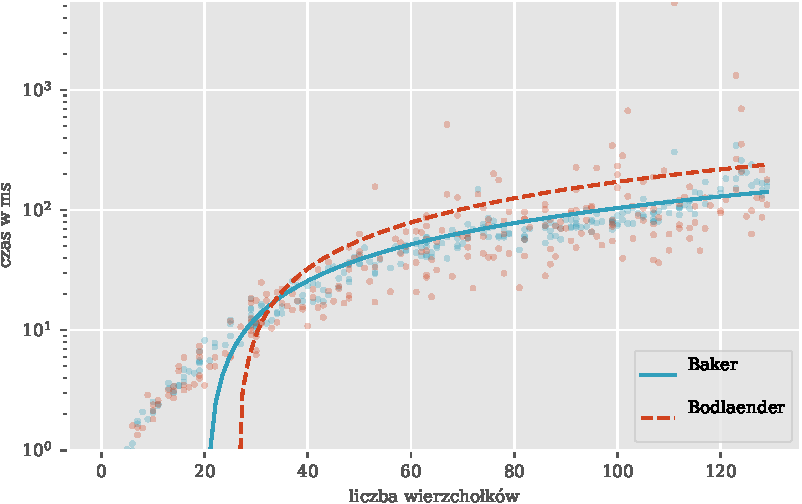
\includegraphics[scale=1.0]{wykresy/is_n.pdf}
    \caption{Czas działania w zależności od liczby wierzchołków grafu dla problemy największego zbioru niezależnego w algorytmie Baker i Bodlaendera.}
    \label{is_n}
\end{figure}

Wyniki testu \texttt{n\_is\_performance} zostały przedstawione na wykresie z rysunku \ref{is_n}. Algorytm Bodlaendera na niektórych grafach osiąga lepsze rezultaty, a na innych zdecydowanie gorsze. Oba algorytmy osiągają duże wartości na tych samych grafach, co sugeruje dużą zewnętrzną planarność tych przykładów. To, który algorytm działa szybciej na danym grafie jest niezależne od liczby wierzchołków, co potwierdza teoretyczną złożoność naszym algorytmów.

\begin{figure}[h!]
    \centering
    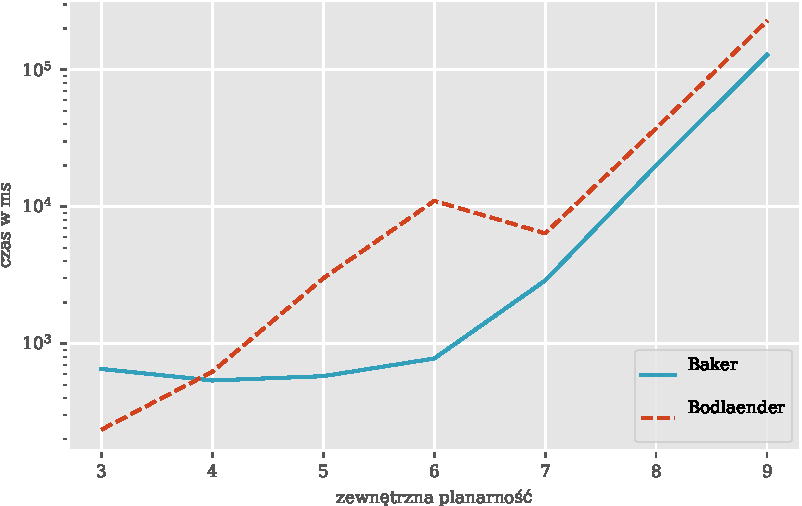
\includegraphics{wykresy/is_k.pdf}
    \caption{Czas działania w zależności od zewnętrznej planarności grafu dla problemu największego zbioru niezależnego w algorytmie Baker i Bodlaendera.}
    \label{is_k}
\end{figure}

Wyniki kolejnego testu \texttt{kouter\_is\_performance} zastały przedstawione na wykresie z rysunku \ref{is_k}. Algorytm Baker osiąga bardzo podobny czas dla grafów o zewnętrznej planarności od $3$ do $6$, co może świadczyć o tym, że czas potrzebny do zbudowania drzew dla tych grafów jest znacznie większy niż czas potrzebny na wyliczenie wyniku. Algorytm Bodlaendera stabilnie osiąga coraz wyższy czas dla coraz wyższej zewnętrznej planarności grafów poza wyższym wynikiem dla grafów $6$-zewnętrznie planarnych. Duży wynik dla tych grafów może świadczyć o wyższej szerokości drzewowej grafów znajdujących się w tej partii, ponieważ szerokość drzewowa jest ograniczona tylko od góry przez $3k-1$, a w praktyce często jest dużo niższa. Algorytm Bodlaendera już przy $k = 4$ zaczyna działać wolniej niż algorytm Baker, co również potwierdza teoretyczną złożoność algorytmów.

\begin{figure}[h!]
    \centering
    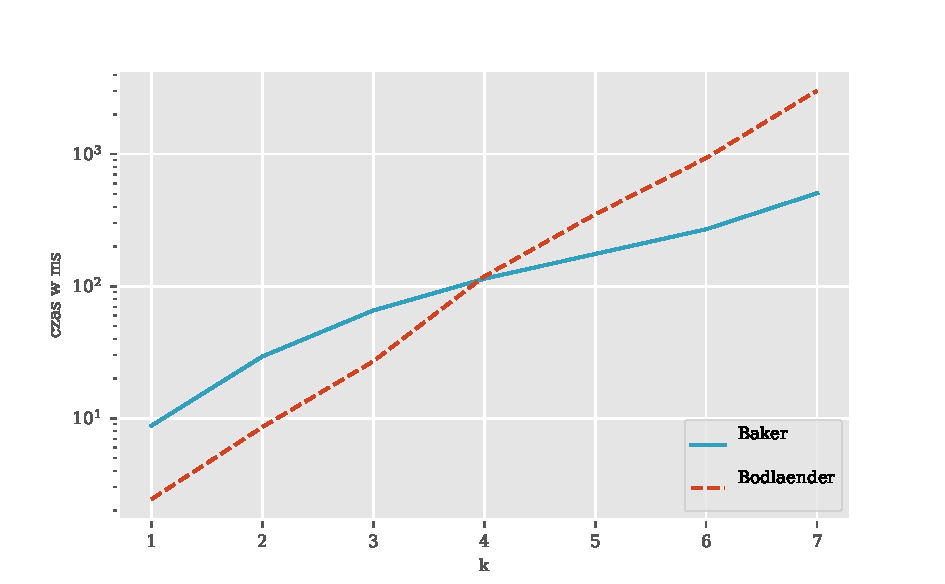
\includegraphics{wykresy/is_ptas.pdf}
    \caption{Czas działania w zależności od $k$ grafu dla techniki Baker używając algorytmu Baker i Bodlaendera do wyliczenia największego zbioru niezależnego.}
    \label{is_ptas}
\end{figure}

Wyniki testu \texttt{ptas\_is\_performance} zostały przedstawione na wykresie z rysunku \ref{is_ptas}. Osiągamy bardzo podobne wyniki do poprzedniego testu. Dla obu algorytmów obserwujemy prawie liniowe wykresy, co świadczy o ich wykładniczym wzroście. Algorytm Baker zaczyna od wolniejszego czasu z powodu konstrukcji koniecznych do jego działania, jednak już przy $k=4$ zaczyna działać szybciej od algorytmu Bodlaendera dzięki niższej podstawie w części wykładniczej złożoności. Technika Baker używająca algorytmu Baker osiąga stosunkowo krótki czas działania nawet przy dosyć dużym $k$, co czyni ją sensowną możliwością nawet w praktycznych zastosowaniach. 

\begin{figure}[h!]
    \centering
    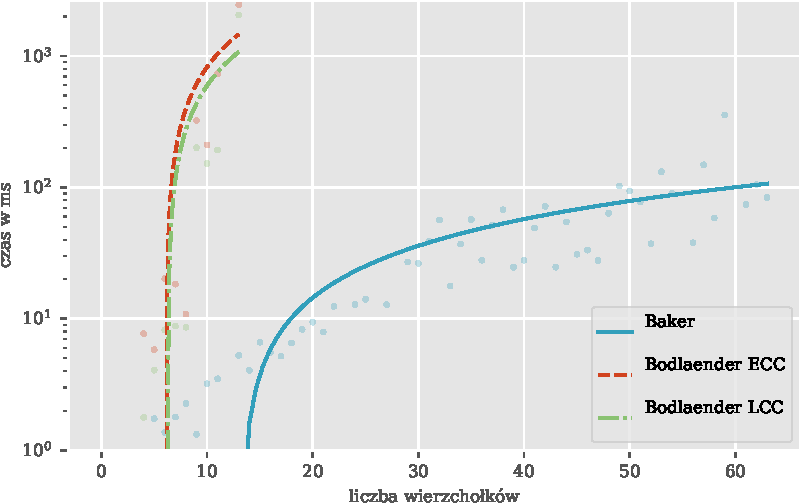
\includegraphics{wykresy/ds_n.pdf}
    \caption{Czas działania w zależności od liczby wierzchołków grafu dla zbioru dominującego w algorytmie Baker i w obu wersjach algorytmu Bodlaendera.}
    \label{ds_n}
\end{figure}

Wyniki testu \texttt{ptas\_is\_results} zostały przedstawione na wykresie z rysunku \ref{is_ptas_res}. Wynik zwracany przez technikę Baker zachowuje się tak jak można się było tego spodziewać, czyli jak wykres funkcji $f(x)=\frac{x}{x+1}$, gwałtownie poprawiając wynik dla pierwszych $k$, a następnie prawie nie zmieniając wartości od $k=6$. Jeśli jednak interesuje nas ograniczenie górne największego wyniku, to osiągamy podobne rezultaty używając $k=1$, co $k=8$.

\begin{figure}[h!]
    \centering
    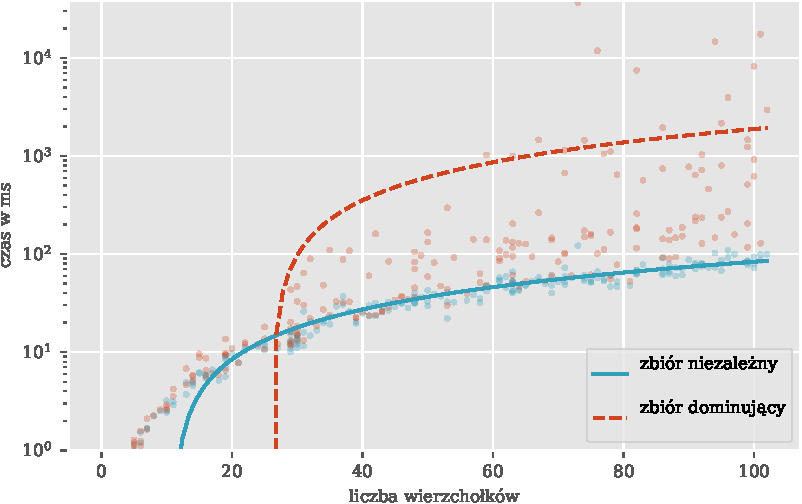
\includegraphics{wykresy/is_ds_n.pdf}
    \caption{Czas działania w zależności od liczby wierzchołków grafu dla zbioru dominującego w algorytmie Baker i w obu wersjach algorytmu Bodlaendera.}
    \label{is_ds_n}
\end{figure}

Wyniki testu \texttt{n\_ds\_performance} zostały przedstawione na wykresie z rysunku \ref{ds_n}. Wyniki te potwierdzają bardzo dużą złożoność algorytmu Bodlaendera dla problemu największego zbioru niezależnego. Algorytm Baker działa nieporównywalnie szybciej nawet na grafach o dużo większej liczbie wierzchołków.

\begin{figure}[h!]
    \centering
    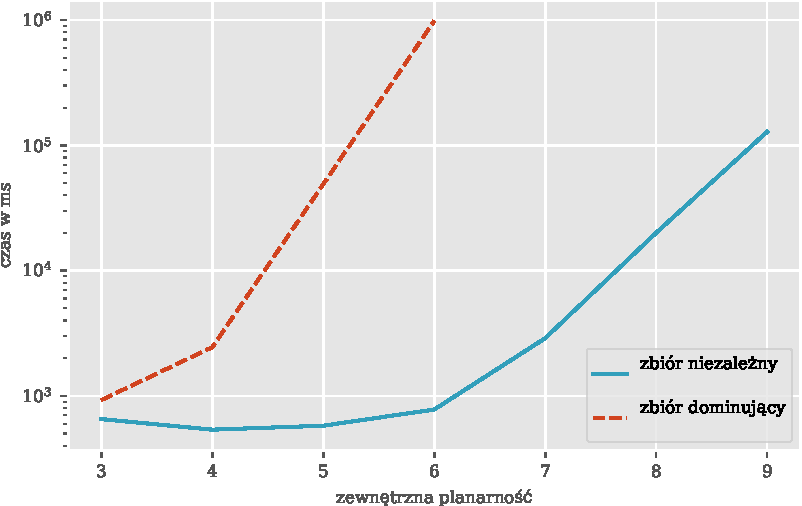
\includegraphics{wykresy/is_ds_k.pdf}
    \caption{Czas działania w zależności od zewnętrznej planarności grafu dla problemu największego zbioru niezależnego i problemu najmniejszego zbioru dominującego w algorytmie Baker.}
    \label{is_ds_k}
\end{figure}

Wyniki testu \texttt{n\_baker\_performance} zostały przedstawione na wykresie z rysunku \ref{is_ds_n}. Algorytm Baker rozwiązując problem najmniejszego zbioru dominującego jest zdecydowanie wolniejszy niż podczas rozwiązywania problemu największego zbioru niezależnego. Mimo teoretycznej niższej złożoności jest również wolniejszy od algorytmu Bodlaendera dla problemu największego zbioru niezależnego, co najprawdopodobniej jest spowodowane niższą od górnego ograniczenia szerokością drzewową grafów, na których został wykonany test.

\begin{figure}[h!]
    \centering
    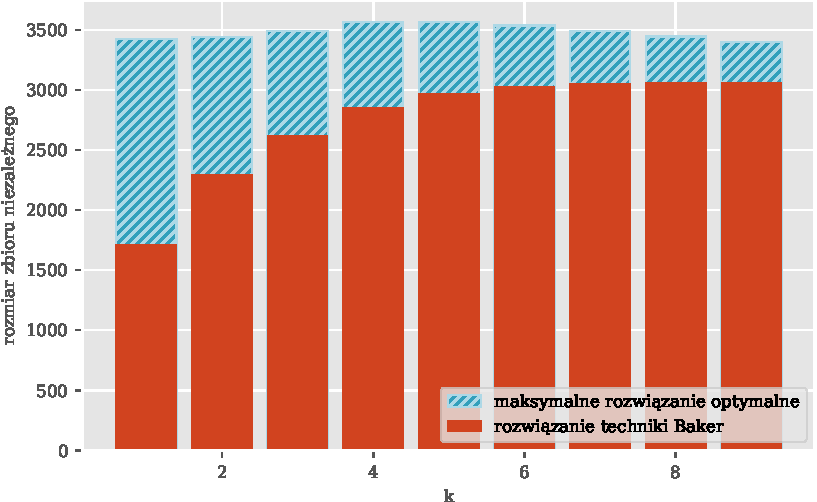
\includegraphics{wykresy/is_ptas_res.pdf}
    \caption{Porównanie wyniku otrzymanego z techniki Baker z ograniczeniem górnym $OPT$ dla problemu największego zbioru niezależnego.}
    \label{is_ptas_res}
\end{figure}

\begin{figure}[h!]
    \centering
    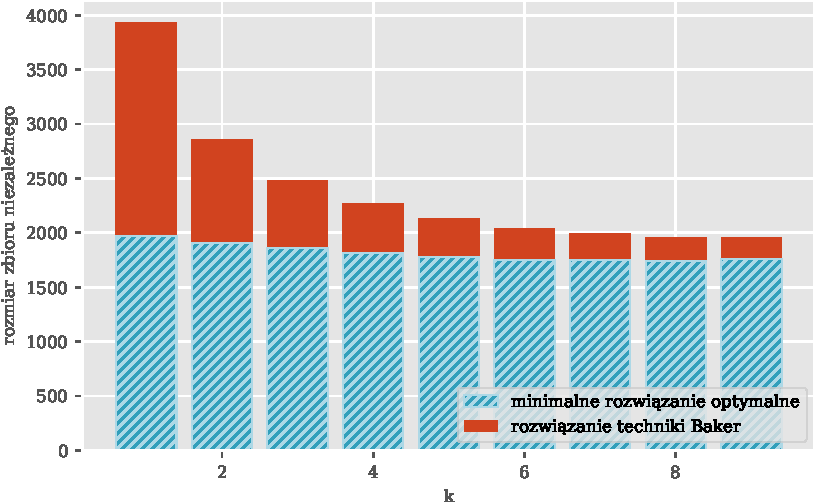
\includegraphics{wykresy/vc_ptas_res.pdf}
    \caption{Porównanie wyniku otrzymanego z techniki Baker z ograniczeniem dolnym $OPT$ dla problemu najmniejszego pokrycia wierzchołkowego.}
    \label{vc_ptas_res}
\end{figure}

Wyniki testu \texttt{kouter\_baker\_performance} zostały przedstawione na wykresie z rysunku \ref{is_ds_k}. Nawet algorytm Baker przy rozwiązywaniu problemu najmniejszego zbioru dominującego okazuje się bardzo niepraktyczny dla grafów o większym współczynniku zewnętrznej planarności.


Wyniki testu \texttt{ptas\_vc\_results} zostały przedstawione na wykresie z rysunku \ref{vc_ptas_res}. Obserwujemy podobną tendencję jak w poprzednim teście: wielkość rozwiązania techniki Baker znacząco maleje dla wyższych $k$, jednak ograniczenie dolne na rozwiązanie optymalne pozostaje prawie niezmienne.

Podsumowując wszystkie testy algorytm Baker prawie w każdej sytuacji działa znacznie szybciej od algorytmu Bodlaendera. Ten ostatni osiąga akceptowalny czas działania tylko dla problemów z klasy $ECC$, które potrafi rozwiązać w czasie liniowym od liczby wierzchołków. Technika Baker natomiast okazuje się dość praktycznym i stosowalnym do wielu problemów schematem aproksymacyjnym.

\section{Podsumowanie}
Algorytm Baker jest skomplikowany i trudny w implementacji. Składa się z wielu kroków, z których każdy wymaga dużej ostrożności, ponieważ błąd w jednym z nich może objawić się dopiero później, co powoduje trudności w identyfikacji i rozwiązywaniu błędów. Dodatkowo wymaga ciągłego operowania na embeddingu grafu, co bardzo komplikuje nawet podstawowe operacje, takie jak dodawanie krawędzi. Mimo swoich wad jest on jednak bardzo skuteczny nie tylko w teorii, ale może być również stosowany w praktyce dla grafów nawet średniej wielkości.

Algorytm Bodlaendera jest przeciwieństwem algorytmu Baker. Jest łatwy w implementacji (nawet wliczając konieczność tworzenia dekompozycji drzewowej), ale jego złożoność czyni go bardzo niepraktycznym dla większego współczynnika zewnętrznej planarności grafu. Dodatkowo algorytm ten ma zapewnioną taką złożoność dla mniejszej liczby problemów niż algorytm Baker.

Jeśli techniką Baker chcemy osiągnąć przybliżenie wyniku lepsze niż $\frac{5}{6}$ stosowanie algorytmu Baker daje znacznie lepsze rezultaty czasowe. Stosowanie algorytmu Bodlaendera w technice Baker jest optymalne tylko wtedy, gdy nie zależy nam dobrym oszacowaniu rozwiązania optymalnego. 





%%%%%%%%%%%%%%%%%%%%%% \textendash- Bibliografia i indeksy \textendash- %%%%%%%%%%%%%%%%%%%%%%
\bibliographystyle{plain}
\bibliography{bib}



\end{document}
